
\chapter{Two-Dimensional SEAS model}
In a second step we consider a trivial SEAS model with only two dimensions and square, symmetric tectonic plates.

\section{Physical Description}
\label{ssec:physicalDescriptionSEAS2D}
--- write down Poisson/elasticity equation for the domain --- \\
--- rate and state laws for the fault --- \\
describe what all variables mean and stuff...
Ageing law: 
\begin{equation}
    \dot{\psi} = g(\psi, V) = \frac{bV_0}{L}e^{\frac{f_0 - \psi}{b}} - \frac{V}{V_0}
\end{equation}
Friction law: 
\begin{equation}
    0 = \tau(U) - a\sigma_n(U) \text{arsinh}\left(\frac{V}{2V_0}e^{\frac{\psi}{a}}\right) - \eta V
\end{equation}


\section{BP1 problem}
--- read more about BP1 and find good citations --- \\
The displacement is applied orthogonal to the represented plane, thus, if the mesh is located in the X-Y plane, each element has one traction, velocity and displacement component acting in the Z direction. In this model problem, the represented tectonic plates have a symmetric layout and move in opposite direction, as one moves into the plane and the other one out of the plane. Therefore, it is enough to consider only one half of the domain, as the results in the other half will be identical, but with opposite sign. \autoref{fig:mesh_BP1_200_fault_elements} depicts the half-domain on which the solution is calculated. The fault here is located on the left side of the domain.
\begin{figure}[H]
    \centering
    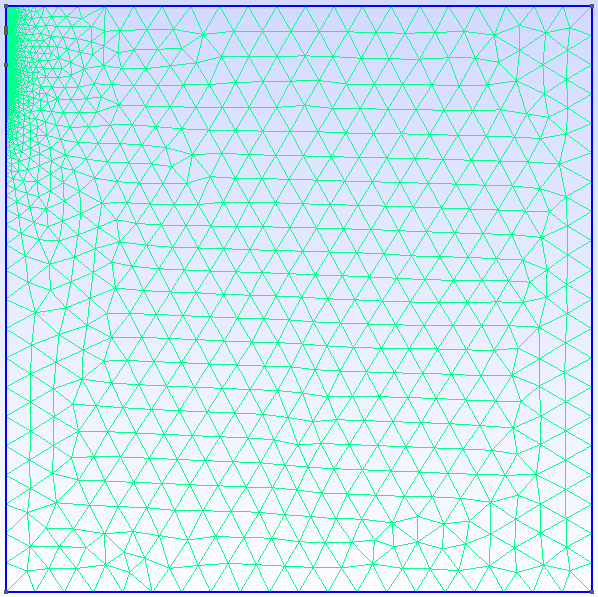
\includegraphics[width=0.4\textwidth]{images/BP1_MESH_200.png}
    \caption{Space discretization of the BP1 problem with 200 elements on the fault}
    \label{fig:mesh_BP1_200_fault_elements}
\end{figure}

In the considered example, we choose the mesh such that there are 200 elements at the fault. The lower end of the plates is pulled with a constant velocity $V_0 = 10^{-6} m\cdot s^{-1}$. 

\section{Formulation of the Discontinous Galerkin}

--- write something about DG --- \\ 


The numerical integration is achieved with the Gaussian quadrature. For that, Gauss-Legendre polynomials up to order $p$ are chosen to interpolate relevant values on each element. Dependent on the chosen order $p$, the solution has to be calculated at different points $x_i$ within the element and, associated with the correct weights to interpolate the data over the entire element, the integration is exact with respect to the interpolation polynomials. \\
--- write more about GQ --- \\

To solve the Poisson equation, it is necessary to evaluate the integral over the entire element and to handle boundary conditions and the fault, the integral over the edges of the element is needed. 


\section{First Order Differential Equation}
The problem stated in \autoref{ssec:physicalDescriptionSEAS2D} is a first order DAE, as the involving terms only depend on the unknown quantities and at most there first time derivatives:
\begin{align}
    \dot{S_i} &= V_i \label{eq:SEASDAE_dV_dt} \\
	\dot{\psi_i} &= g(\psi_i, V_i) =\frac{bV_0}{L}\left(e^{\frac{f_0-\psi_i}{b}} - \frac{V_i}{V_0}\right) \label{eq:SEAS_DAE_ageing_law} \\
	0 &= f_i(U,S,\psi,V) = \tau_i(U,S) - a\sigma_n\text{arsinh}\left(\frac{V_i}{2V_0}e^{\frac{\psi_i}{a}}\right) -\eta V_i \label{eq:SEASDAE_frictionLaw}\\
    0 &= AU - b(S) \label{eq:SEAS_DAE_AU=b}  
\end{align}
The index $i\in[0,n]$ refers to all interpolation points of the elements located on the fault, meaning that $S_i$, $V_i$ and $\psi_i$ are respectively the slip, the velocity and the value of the state variable on the fault. The matrix-vector system in \autoref{eq:SEAS_DAE_AU=b} stems from the DG formulation of the Poisson problem and needs to be solved for all nodes with index $j\in[0,N]$ in the DG domain. Usually, there are much more nodes in the full domain then purely on the fault, so $n \ll N$. The slip $S_i$ at the fault is related to the displacement $U_j$ by $\llbracket U_j \rrbracket = U_j^+ - U_j^- = -S_i$, where $j$ is the index of the fault node $i$ in the discretization of the full DG domain. The displacements $U_j^+$ and $U_j^-$ correspond to the displacements on the two sides of the fault, for the current symmetric problem, they have the same magnitude with opposite signs. Outside of the fault, the term $S$ is used to enforce boundary conditions on the domain, and typically increases with time, simulating constant tectonic movements of the plates. Nodes on the fault will first resist to this environment slip and when the forces reach a certain level, an earthquake is triggered. \\
 

\subsection{Formulation as a first order ODE}
The first approach to solve the problem is to formulate the system as a classical ODE. The solution vector contains the values for the slip and for the state variable, and at each timestep, the the slip rate $V$ is calculated from \autoref{eq:SEASDAE_frictionLaw} from the state with an iterative solver.
\begin{align}
	\label{eq:ODE_formulation_SEAS}
	x &= \begin{pmatrix}
		S \\ \psi
	\end{pmatrix} & \dot{x} &= \begin{pmatrix}
								  \dot{S} \\ \dot{\psi}
							   \end{pmatrix} = \begin{pmatrix}
												   V(S,\psi) \\ g(\psi, V)
											   \end{pmatrix} = F
\end{align} 
Such a formulation allows us to use many well-known and proved numerical schemes, both implicit and explicit. 

\subsection{Formulation as a DAE}
The ODE form looks pretty and like an easy-to-tackle numerical problem, but may run into some trouble because of the implicit evaluation of the slip rate, which is treated independently of the numerical integration. Alternatively, the friction law could be solved for the slip rate together with the time-variant solution components. The solution vector is then extended by one quantity, and the evaluation of the slip rate with a separate iterative does not occur anymore.
\begin{align}
	\label{eq:DAE_formulation_SEAS}
	x &= \begin{pmatrix}
			S \\ \psi \\ V
		 \end{pmatrix} & \dot{x} &= \begin{pmatrix}
										\dot{S} \\ \dot{\psi} \\ 0
									\end{pmatrix} = \begin{pmatrix}
										V \\ g(\psi, V) \\ f(S,\psi,V)
									\end{pmatrix}
\end{align}
This system cannot be used anymore with pure explicit solvers, since no time discretization can be set up for the algebraic equation. It is however well-suited for implicit methods, which iteratively solve for the time-variant quantities $S$ and $\psi$ as well for the algebraic state $V$. A notable advantage of this formulation is that the tolerances of the numerical solver can be specified independently for $S$, $\psi$ and $V$, whereas in the ODE formulation of the problem, the error control is limited to the parameters $S$ and $\psi$. \\
The PETSc interface requires us to provide a DAE in the form
\begin{align}
	F(t, x,\dot{x}) = G(t,x) 
\end{align}
where the left-hand side function $F()$ depends on the solution vector and its time derivative whereas the right-hand side function $G()$ only depends on the solution vector. For now, we choose a fully implicit formulation of the problem, in which $G()$ vanishes. The DAE can then be expressed in the following way: 
\begin{align}
\label{eq:DAE_extended_formulation_SEAS}
	x &= \begin{pmatrix}
		S \\ \psi \\ V
	\end{pmatrix} & F(t, x,\dot{x}) &= \begin{pmatrix}
	 	V - \dot{S} \\ g(\psi, V) - \dot{\psi}  \\ f(S,\psi,V)
	\end{pmatrix} = \begin{pmatrix}
		0 \\ 0 \\ 0
	\end{pmatrix} = G(t,x)
\end{align}

Another class of solvers, the so called IMEX (implicit-explicit) solvers [cite IMEX], offer an interesting approach to numerically solve this problem, by mixing an implicit, iterative method for the algebraic states with an explicit method for the remaining simple time-dependent quantities. Technically, the function $F()$ is expected to be integrated implicitly, while the right-hand side function $G()$ is solved explicitly. In the given formulation, the right hand side is equal to 0, this means that the system has to be solved fully implicitly and the advantages of IMEX methods cannot be used here. 

\subsection{Compact formulation as a DAE}
It is important to remember that the slip rate is the time derivative of the slip, so the variables $\dot{S}$ and $V$ are equal and can be interchanged in the problem formulation. As such, the friction law can be solved directly for $\dot{S}$ and the term $V$ is not required anymore. The solution vector then remains with the components of the slip $S$ and of the state variable $\psi$, as previously in the ODE formulation.
 \begin{align}
	\label{eq:DAE_compact_formulation_SEAS}
	x &= \begin{pmatrix}
			S \\ \psi
	     \end{pmatrix} & F(t, x,\dot{x}) &= \begin{pmatrix}
												f(S,\psi,V) \\ \dot{\psi} - g(\psi, V)
											\end{pmatrix} = \begin{pmatrix}
																0 \\ 0
															\end{pmatrix} = G(t,x)
\end{align}
As in the developed DAE formulation, the friction law is solved along with time-variant quantities $S$ and $\psi$. It therefore requires an iterative solver method from an implicit time solver and it can be used only with an implicit integrator. \\

\section{Formulation of the Jacobian}
To use implicit time solvers, the Jacobian matrix of the right-hand side of the ODE in (\ref{eq:SEAS_DAE_ageing_law}) and (\ref{eq:SEASDAE_dV_dt}) has to be computed in the Newton iteration. In general, if it is unknown, it is approximated along with the solution during the Newton iteration using for instance a Broyden iteration [cite Broyden]. However, this impairs the convergence speed of the Newton iteration compared to the analytical expression. It is especially relevant if a DAE formulation of the problem is chosen, for which an iterative solver is indispensable. 

\subsection{Analytical Derivation of the Jacobian matrix}
\label{ssec:AnalyticalDerivationOfTheJacobianMatrix}
Next, we try to derive an analytical expression of the Jacobian for both the ODE and the DAE formulation of the problem, so that the Newton iterations when using implicit methods can be solved efficiently.  

\subsubsection{Jacobian of the ODE system}
\label{sssec:Jacobian_ODE}
For the ODE formulation in \autoref{eq:ODE_formulation_SEAS}, it is not straightforward to calculate the Jacobian matrix because of the implicit evaluation of the slip rate within the right-hand side function. The matrix $\mathbf{J}_{\psi,S}(F)$ consists of four block matrices, which each contains the Jacobians related to the two quantities:
\begin{equation}
	\label{eq:Jacobian_ODE_formulation}
	\mathbf{J}_{\psi_j,S_j}\left(F_i\left(\psi,V(\psi,S)\right)\right) = \begin{pmatrix} 
	\frac{\partial V_i}{\partial S_j} &
	\frac{\partial V_i}{\partial \psi_j} \\ 
	\frac{\partial g(\psi_i,V_i)}{\partial S_j} &
	\frac{\partial g(\psi_i,V_i)}{\partial \psi_j}  \end{pmatrix}
\end{equation}
In a first step, the partial derivatives of the slip rate $V$ will be calculated. As this quantity is obtained implicitly from the friction law in \autoref{eq:SEASDAE_frictionLaw}, the implicit function theorem has to be applied. The function $f()$ is continuously differentiable and its Jacobian matrix with respect to the slip rate $\frac{\partial f}{\partial V}$ is invertible. Indeed, from the analytic expression in \autoref{eq:partial_df_dV}, it appears that the matrix is diagonal and its entries are all non-zero. All necessary conditions to apply the implicit function are fulfilled and it states that the partial derivatives of $V$ are given by the product:
\begin{align}
	\frac{\partial V}{\partial S} &= -\left(\frac{\partial f}{\partial V}\right)^{-1}\frac{\partial f}{\partial S} \\ 
	\frac{\partial V}{\partial \psi} &= -\left(\frac{\partial f}{\partial V}\right)^{-1}\frac{\partial f}{\partial \psi} 
\end{align}
Two of the occurring Jacobian matrices can be easily obtained from the respective derivatives of the friction law. 
\begin{equation}
\frac{\partial f_i(S,\psi,V)}{\partial \psi_j} = \left( -\frac{\sigma_n}{2V_0} \frac{Ve^{\frac{\psi_i}{a}}}{\sqrt{\frac{e^{\frac{2\psi_i}{a}}V_i^2}{4V_0^2}+1}}\right)\delta_{ij} 
\label{eq:partial_df_dpsi}
\end{equation}	
\begin{equation}
\frac{\partial f_i(S,\psi,V)}{\partial V_j} = \left( -\frac{\sigma_na}{2V_0} \frac{e^{\frac{\psi_i}{a}}}{\sqrt{\frac{e^{\frac{2\psi_i}{a}}V_i^2}{4V_0^2}+1}}-\eta\right)\delta_{ij} 
\label{eq:partial_df_dV}
\end{equation}
Since $\frac{\partial f}{\partial V}$ is a diagonal matrix, its inverse is very easy to calculate and does not require to solve a linear system of equations. The evaluation of the last missing partial derivative is more complex to obtain and will be one reason for a partial filling of the Jacobian matrix.
\begin{align}
\label{eq:partialDerivative_df_dS}
\frac{\partial f_i}{\partial S_j} = \frac{d \tau_i(U)}{d S_j} = \frac{\partial \tau_i(U)}{\partial U_k}\frac{\partial U_k}{\partial S_j} + \frac{\partial \tau_i(U)}{\partial S_j}
\end{align}
The problem shifted to calculate the partial derivative $\frac{\partial U}{\partial S}$. Since $U = A^{-1}b(S)$ and the matrix $A$ does not depend on $S$, we just need to find the derivative of $b(S)$. We get, for elements on the fault:
\begin{align}
\frac{\partial b_i(S)}{\partial S_j} &= \frac{\partial }{\partial S_j}\int_e \eta \{\{c_{mnkl}\epsilon_{kl}(w)\eta_n^e\}\}\llbracket U_m \rrbracket + \frac{\delta_e}{|e|^\beta}\llbracket U_m \rrbracket\llbracket w_m \rrbracket dx
\end{align}
As already stated earlier, we have $\llbracket U_i \rrbracket = -S_i$, therefore we can straight eliminate this term. On all other interpolation points not located on the fault, the right hand side $b$ does not depend on the fault displacement $S$ and the derivatives at these points consequently vanish. We then obtain:
\begin{equation}
\frac{\partial b_i(S)}{\partial S_j} = -\int_e 
\eta  \{\{c_{jnkl}\epsilon_{kl}(w)\eta_n^e\}\} +
\frac{\delta_e}{|e|^\beta}\llbracket w_j \rrbracket dx
\end{equation}
This expression can be calculated by plugging the unit vector $e^i$ as argument of the right-hand side vector $b$. The Jacobian term $\frac{\partial U_i}{\partial S_j}$ is therefore evaluated by applying the solver method of the Poisson problem to the unit vectors as slips. We get:
\begin{equation}
\frac{\partial U_i}{\partial S_j} = A_{ik}^{-1}b_k(e^i)
\end{equation}
The traction term $\tau(U,S)$ is calculated as $\tau = \mu \frac{\partial u}{\partial x_i}n_i$, and is numerically approximated on the nodal basis as $\tau_p = M_{rp}^{-1}e_{qr}^Tw_q(\nabla u)_{kq}n_{kq}$, where $M$ is the mass matrix of the fault basis, $e^T$ maps from fault to quadrature points, $w$ are the quadrature weights and $n$ is the normal at the quadrature points. The gradient of $u$ is approximated by $(\nabla u)_{pq} = \frac{1}{2}\left(D_{lpq}^0u_l^0 + D_{lpq}^1u_l^1\right) + c_0\left(E_{lq}^0u_l^0 - E_{lq}^1u_l^1 - f_q\right)n_{pq}$. The tensor $E$ maps from the quadrature points to the element basis and $D$ is its gradient and the superscripts $0$ and $1$ refer to the adjacent elements on opposite sides of the fault. The term $f_q$ denotes the actual slip transformed to the quadrature points. The evaluation of the derivative of the traction with respect to the displacement requires to derivate the gradient of the displacement with respect to itself. We obtain: 
\begin{align}
\frac{(\nabla u)_{pq}}{\partial u_k} &= \frac{1}{2}\left(D_{lpq}^0\frac{\partial u_l^0}{\partial u_k} + D_{lpq}^1\frac{\partial u_l^1}{\partial u_k}\right) + c_0\left(E_{lq}^0\frac{\partial u_l^0}{\partial u_k} - E_{lq}^1\frac{\partial u_l^1}{\partial u_k}\right)n_{pq} \\
&= \frac{1}{2}\left(D_{lpq}^0\delta_{lk}^0 + D_{lpq}^1\delta_{lk}^1\right) + c_0\left(E_{lq}^0\delta_{lk}^0 - E_{lq}^1\delta_{lk}^1\right)n_{pq} \\
&= \frac{1}{2}\left(D_{kpq}^0 + D_{kpq}^1\right) + c_0\left(E_{kq}^0 - E_{kq}^1\right)n_{pq} 
\end{align}
And further we get: 
\begin{equation}
\frac{\partial \tau_p}{\partial u_l} = M_{rp}^{-1}e_{qr}^Tw_q
\frac{(\nabla u)_{kq}}{\partial u_l}n_{kq}
\end{equation}
In addition, the traction needs to be derivated with respect to the current slip directly for the term $\frac{\partial \tau_i(U)}{\partial S_j}$, which is contained in the term $f_q = e_{qj}S_j$. It appears again in the gradient, so its derivative with respect to the slip is also needed. 
\begin{align}
\frac{(\nabla u)_{pq}}{\partial S_j} = -c_0 \frac{\partial f_q}{\partial S_j}n_{pq} 
= -c_0 e^T_{qk}\frac{\partial S_k}{\partial S_j}n_{pq} 
= -c_0 e^T_{qj}n_{pq} \\	
\end{align}
With this expression, we obtain: 
\begin{equation}
\frac{\partial \tau_p}{\partial S_j} = -M_{rp}^{-1}e_{qr}^Tw_qc_0e^T_{qj}n_{kq}n_{kq}
\end{equation}
This derivative term does not depend on the current slip anymore but only on the geometry of the discretization, so it can be calculated once at the beginning of the simulation. All components of the remaining partial derivative in \autoref{eq:partialDerivative_df_dS} are now available and the Jacobian matrices of the slip rate with respect to the slip and to the state variable can be calculated. \\
To express the full Jacobian matrix of the ODE in \autoref{eq:Jacobian_ODE_formulation}, the partial derivatives of the ageing law $g(\psi, V)$ are still missing. They can be expressed in term of the already known partial derivatives: 
\begin{align}
	\frac{\partial g_i}{\partial S_j} &= -\frac{b}{L}\frac{\partial V}{\partial S} \\
	\frac{\partial g_i}{\partial S_j} &= -\frac{V_0}{L}e^{\frac{f_0 - \psi}{b}}\delta_{ij} -
										  \frac{b}{L}\frac{\partial V}{\partial \psi}
\end{align}



\subsubsection{Jacobian of the DAE system}
\label{sssec:Jacobian_DAE}
For the DAE formulation of the system in \autoref{eq:DAE_extended_formulation_SEAS}, another approach can be chosen to calculate the Jacobian matrix of the system. With now three different components in the solution vector, the Jacobian matrix contains the partial derivatives with respect to the slip rate in addition to the slip and to the state variable. Similarly, the function $F$ on which the Jacobian is applied is extended by the friction law. Each block $i,j$ in the structure of the Jacobian is given by:
\begin{equation}
	\label{eq:Jacobian_DAE_formulation}
	\mathbf{J}_{S_j,\psi_j,V_j}F_i(S,\psi,V) = 	\begin{pmatrix}
											\frac{\partial V_i}{\partial S_j} & \frac{\partial V_i}{\partial \psi_j} & \frac{\partial V_i}{\partial V_j} \\
											\frac{\partial g_i(\psi,V)}{\partial S_j} & \frac{\partial g_i(\psi,V)}{\partial \psi_j} & \frac{g_i(\partial \psi,V)}{\partial V_j} \\
											\frac{\partial f_i(S,\psi,V)}{\partial S_j} & \frac{\partial f_i(S,\psi,V)}{\partial \psi_j} & \frac{\partial f_i(S,\psi,V)}{\partial V_j}
										\end{pmatrix}
\end{equation}
In the previous section, a complicated approach had to be followed to obtain the derivative for the slip rate because of the nonlinear friction law, which was indirectly solved for each evaluation of the slip rate. Since the slip rate is now obtained directly from the solution vector $x$ and not from an iterative solver for the friction law, all its partial derivatives except with each component itself vanish. 

\begin{align}	
	\frac{\partial V_i}{\partial S_j} &= 0 & \frac{\partial V_i}{\partial \psi_j} &= 0 & \frac{\partial V_i}{\partial V_j} &= \delta_{ij}
\end{align}

Similarly, the partial derivatives of the ageing law can be directly evaluated from its definition in \autoref{eq:SEAS_DAE_ageing_law}.
\begin{align}
	\frac{\partial g_i(\psi,V)}{\partial S_j} &=  0 &
	\frac{\partial g_i(\psi,V)}{\partial\psi_j} &= -\frac{V_0}{L}e^{\frac{f_0-\psi_i}{b}}\delta_{ij} &	
	\frac{\partial g_i(\psi,V)}{\partial V_j} &= -\frac{b}{L} \delta_{ij}
\end{align}
For the friction law, the Jacobian matrices have already been calculated in \autoref{eq:partial_df_dpsi} for $\frac{\partial f(S,\psi,V)}{\partial psi}$, in \autoref{eq:partialDerivative_df_dS} for $\frac{\partial f(S,\psi,V)}{\partial S}$ and in \autoref{eq:partial_df_dV} for $\frac{\partial f(S,\psi,V)}{\partial V}$.

This formulation of the Jacobian cannot be directly used in the Newton iteration to calculate the next timestep. Typically, the Jacobian has to be adapted to represent the time-stepping scheme. For instance, the implicit Euler method results requires to solve the nonlinear equation $0 = 1/h(x_n - x_{n+1}) + F(x_{n+1})$ for the solution at the next timestep $x_{n+1}$ and the Jacobian matrix $J_N$ for the corresponding Newton iteration is constructed from $J$. 
\begin{equation}
	J_N = -\frac{1}{h}I + J
\end{equation}
Here, the problem arises that the evolution over time is only defined for two components in the solution vector: the slip $S$ and the state variable $\psi$. The slip rate $V$ needs to be solved algebraically at every Newton iteration, but this component should not be included in the time-stepping scheme. The nonlinear equation to calculate a step of the implicit Euler has to be adapted to include properly the slip rate. 
\begin{align}
	0 = \begin{pmatrix} \frac{1}{h}S_n     \\ \frac{1}{h}\psi_n     \\ 0 \end{pmatrix} - 
		\begin{pmatrix} \frac{1}{h}S_{n+1} \\ \frac{1}{h}\psi_{n+1} \\ 0 \end{pmatrix} + 
		\begin{pmatrix} V_{n+1}            \\ g(\psi_{n+1},V_{n+1}) \\ f(S_{n+1}, \psi_{n+1}, V_{n+1}) \end{pmatrix}
\end{align}
The Jacobian matrix to be used in a Newton iteration to solve this problem has to be changed accordingly.
\begin{align}
	\label{eq:Jacobian_Newton_Iteration_extended_DAE}
	\mathbf{J}_N = 
		\begin{pmatrix} 
		 	-\frac{1}{h}\mathbf{I} & \mathbf{0}            & \mathbf{0} \\ 
		   	\mathbf{0}             &-\frac{1}{h}\mathbf{I} & \mathbf{0} \\ 
		    \mathbf{0}             & \mathbf{0}            & \mathbf{0} 
	 	\end{pmatrix} + 
       	\begin{pmatrix}  
       		\mathbf{J}_S(S)    &  \mathbf{J}_\psi(S)    &  \mathbf{J}_V(S)    \\ 
			\mathbf{J}_S(\psi) &  \mathbf{J}_\psi(\psi) &  \mathbf{J}_V(\psi) \\ 
			\mathbf{J}_S(V)    &  \mathbf{J}_\psi(V)    &  \mathbf{J}_V(V)
		\end{pmatrix} =
		\begin{pmatrix} 
			-\frac{1}{h}\mathbf{I}         &  \mathbf{0} 			            &
			\mathbf{I}                     \\ 
			\mathbf{0}                    & 
			-\frac{1}{h}\mathbf{I} +  \frac{\partial g}{\partial \psi}       &  \frac{\partial g}{\partial V} \\ 
			\frac{\partial f}{\partial S} & \frac{\partial f}{\partial \psi} &  \frac{\partial f}{\partial V} 
		 \end{pmatrix}
\end{align}
If other implicit numerical schemes are used than the implicit Euler, such as higher order BDF methods, $\mathbf{J}_N$ can be easily changed by multiplying the identity matrices $\mathbf{I}$ with a coefficient that depends on the chosen method. Albeit this formulation of the Jacobian matrix is perfectly valid, it is very specific to the SEAS problem and is therefore hard to implement as such within the PETSc framework. \\
To solve general implicit DAEs of the form $F(t,x,\dot{x}) = G(t,x)$, PETSc offers a convenient interface to provide the Jacobian matrices. In fact, three matrices have to be provided. The first Jacobian matrix, denoted by $\mathbf{F}_{\dot{x}}$, corresponds to the variation of the left-hand side function $F()$ with respect to the derivative of the solution vector. The second matrix $\mathbf{F}_x$ describes the variation of the same function under the actual solution vector. Finally, the third Jacobian matrix $\mathbf{G}_x$ represents the variation of the right hand side function $G()$ under the influence of $x$. In our case, the formulation is fully explicit and the right hand side function $G(t,x)$ is zero everywhere, and by extension, its Jacobian matrix $\mathbf{G}_x$ also vanishes. It remains to express the Jacobian matrix of the Newton iteration $\mathbf{J}_N$ in terms of $\mathbf{F}_x$ and $\mathbf{F}_{\dot{x}}$:
\begin{equation}
	\mathbf{J}_N = \frac{dF}{dx_n} = \mathbf{F}_{\dot{x}}\frac{d\dot{x}_n}{dx_n} + \mathbf{F}_x	
\end{equation}
The term $\frac{d\dot{x}_n}{dx_n}$ is a constant scalar and depends only on the chosen time step scheme, which can be denoted by $\sigma$. For the implicit Euler method for instance, we have $\sigma = 1/h$. The Jacobian matrix $\mathbf{F}_x$ is exactly the one expressed in \autoref{eq:Jacobian_DAE_formulation} and $\mathbf{F}_x$ contains negative identity matrices at the entries for the slip $S$ and for the state variable $\psi$.
\begin{align}
	\mathbf{F}_x = \begin{pmatrix} 
		\mathbf{0}                     &  \mathbf{0}                       & 
		\mathbf{I}                    \\ 
		\mathbf{0}                     &  \frac{\partial g}{\partial \psi} & 
		\frac{\partial g}{\partial V} \\ 
		\frac{\partial f}{\partial S}  &  \frac{\partial f}{\partial \psi} &  
		\frac{\partial f}{\partial V} 
	\end{pmatrix} &&&
	\mathbf{F}_{\dot{x}} = \begin{pmatrix} 
		-\mathbf{I}  &  \mathbf{0}  & \mathbf{0} \\ 
  		 \mathbf{0}  & -\mathbf{I}  & \mathbf{0} \\ 
		 \mathbf{0}  &  \mathbf{0}  & \mathbf{0}
	\end{pmatrix}
\end{align}
With this too matrices, the Jacobian matrix for the Newton iteration of the implicit Euler method is exactly the same as calculated in \autoref{eq:Jacobian_Newton_Iteration_extended_DAE}.

\subsubsection{Jacobian of the compact DAE system}
The compact DAE formulation of the problem in \autoref{eq:DAE_compact_formulation_SEAS} needs again to be solved fully implicitly and involves again the three Jacobian matrices, $\mathbf{F}_{\dot{x}}$, $\mathbf{F}_x$ and $\mathbf{G}_x$, where the last one also vanishes because the right-hand side function is zero. The block matrices that appear in this formulation are calculated in exactly the same way as previously but are arranged in a different manner.
\begin{align}
	\mathbf{F}_{\dot{x}}&=  \begin{pmatrix}
								\frac{\partial f}{\partial V} & \mathbf{0} \\
							   -\frac{\partial g}{\partial V} & \mathbf{I}
							\end{pmatrix} & 
	\mathbf{F}_x        &=  \begin{pmatrix}
								\frac{\partial f}{\partial S} & \frac{\partial f}{\partial \psi} \\
								\mathbf{0}                    & \frac{\partial g}{\partial \psi}
							\end{pmatrix} & 
	\mathbf{G}_x        &=  \begin{pmatrix}
								\mathbf{0} & \mathbf{0} \\
							    \mathbf{0} & \mathbf{0}
							\end{pmatrix}
\end{align}

\subsection{Verification of the Jacobian}
The Jacobian matrix is needed to apply implicit numerical methods to solve the SEAS problem. Unlike explicit methods, they evaluate the right hand side of the ODE with the current solution which is not known yet. To calculate the solution vector at a given time step, a nonlinear algebraic equation of the form $\phi(x) = 0$ needs to be solved where $x$ is the solution vector to be determined. The Newton method is often used to solve the equation because of its ease to implement and its second-order convergence. 

\begin{itemize}
	\item Calculate an initial guess $x_0$
	\item Repeat until tolerance is reached $\|\phi(x_n)\| < TOL$: 
	\begin{itemize}
		\item $x_{n+1} = x_n - J_\phi^{-1}(\phi(x_n)) \phi(x_n)$
	\end{itemize} 
\end{itemize}

The matrix $J_\phi^{-1}(f(x_n))$ is the Jacobi matrix of the function $\phi$ evaluated at the point $x_n$. \\
To verify the correctness of the analytic expression of the Jacobi matrix which has been set up in the previous section, it is applied in a Newton iteration to solve one timestep of the implicit Euler method. The function $\phi$ and its Jacobian matrix are given by: 
\begin{align}
	\phi(x) &= -x + x^{(0)} + \Delta t F(x) \\
	J_\phi(x) &= -I + \Delta t J_F(x)
\end{align}
The vector $x$ contains both the components related to the slip $S$ and to the state variable $\psi$ and the right hand-side vector $F(x)$ contains their respective time derivative. The Jacobian of the proposed Newton iteration needs the Jacobian $J_F(x)$ of the right-hand side vector, of which the correctness is evaluated here. The success of the Newton iteration, thus observable second-order convergence, indicates the correctness of the Jacobian matrix. \\
Furthermore, the behavior of the analytic expression of the Jacobian is compared to the behavior of an iterative approximation of it. The Broyden's method \cite{BroydenIteration} provides an enhancement of the Newton method which updates the Jacobian matrix at each iteration without the need of its analytical expression. The main difficulty is to find an appropriate initial guess to achieve a fast convergence. 

\begin{itemize}
	\item Calculate the initial guesses $x_0$ and $J_0$
	\item Repeat until tolerance is reached $\|\phi(x_n)\| < TOL$: 
	\begin{itemize}
		\item $\Delta x_n = x_n - x_{n-1}$ and $\Delta \phi_n = \phi(x_n) - \phi(x_{n-1})$ 
		\item $J_n = J_{n-1} + \frac{\Delta \phi_n - J_{n-1}\Delta x_n}{\|\Delta x_n\|^2} \Delta x_n^T$
		\item $x_{n+1} = x_n - J_n \phi(x_n)$
	\end{itemize} 
\end{itemize}

The motivation behind this update scheme is to minimize the Frobenius norm $\|J_n - J_{n-1}\|_F$. As a matter of simplicity, the initial guess of the Jacobian is obtained with the analytical expression of it, even though its correctness has not yet been shown. Other initialization methods such as finite differences do not lead to convergence of the Broyden method. \\
The experiment has been performed on a symmetric, two-dimensional domain of varying size. The initial guesses for $x$ are obtained with one step of the explicit Euler method with a timestep of $\Delta t = 10^5$s. This time step is large enough to obtain an error to the exact value at this time which needs several Newton iterations to be corrected but still small enough to ensure that the Newton iteration converges at all. The evolution of the residual $\phi(x_n)$ is shown in \autoref{fig:convergenceNewtonAndBroyden}.
 \begin{figure}[H]
 	\centering
 	\begin{subfigure}{0.32\textwidth}
 		\centering
 		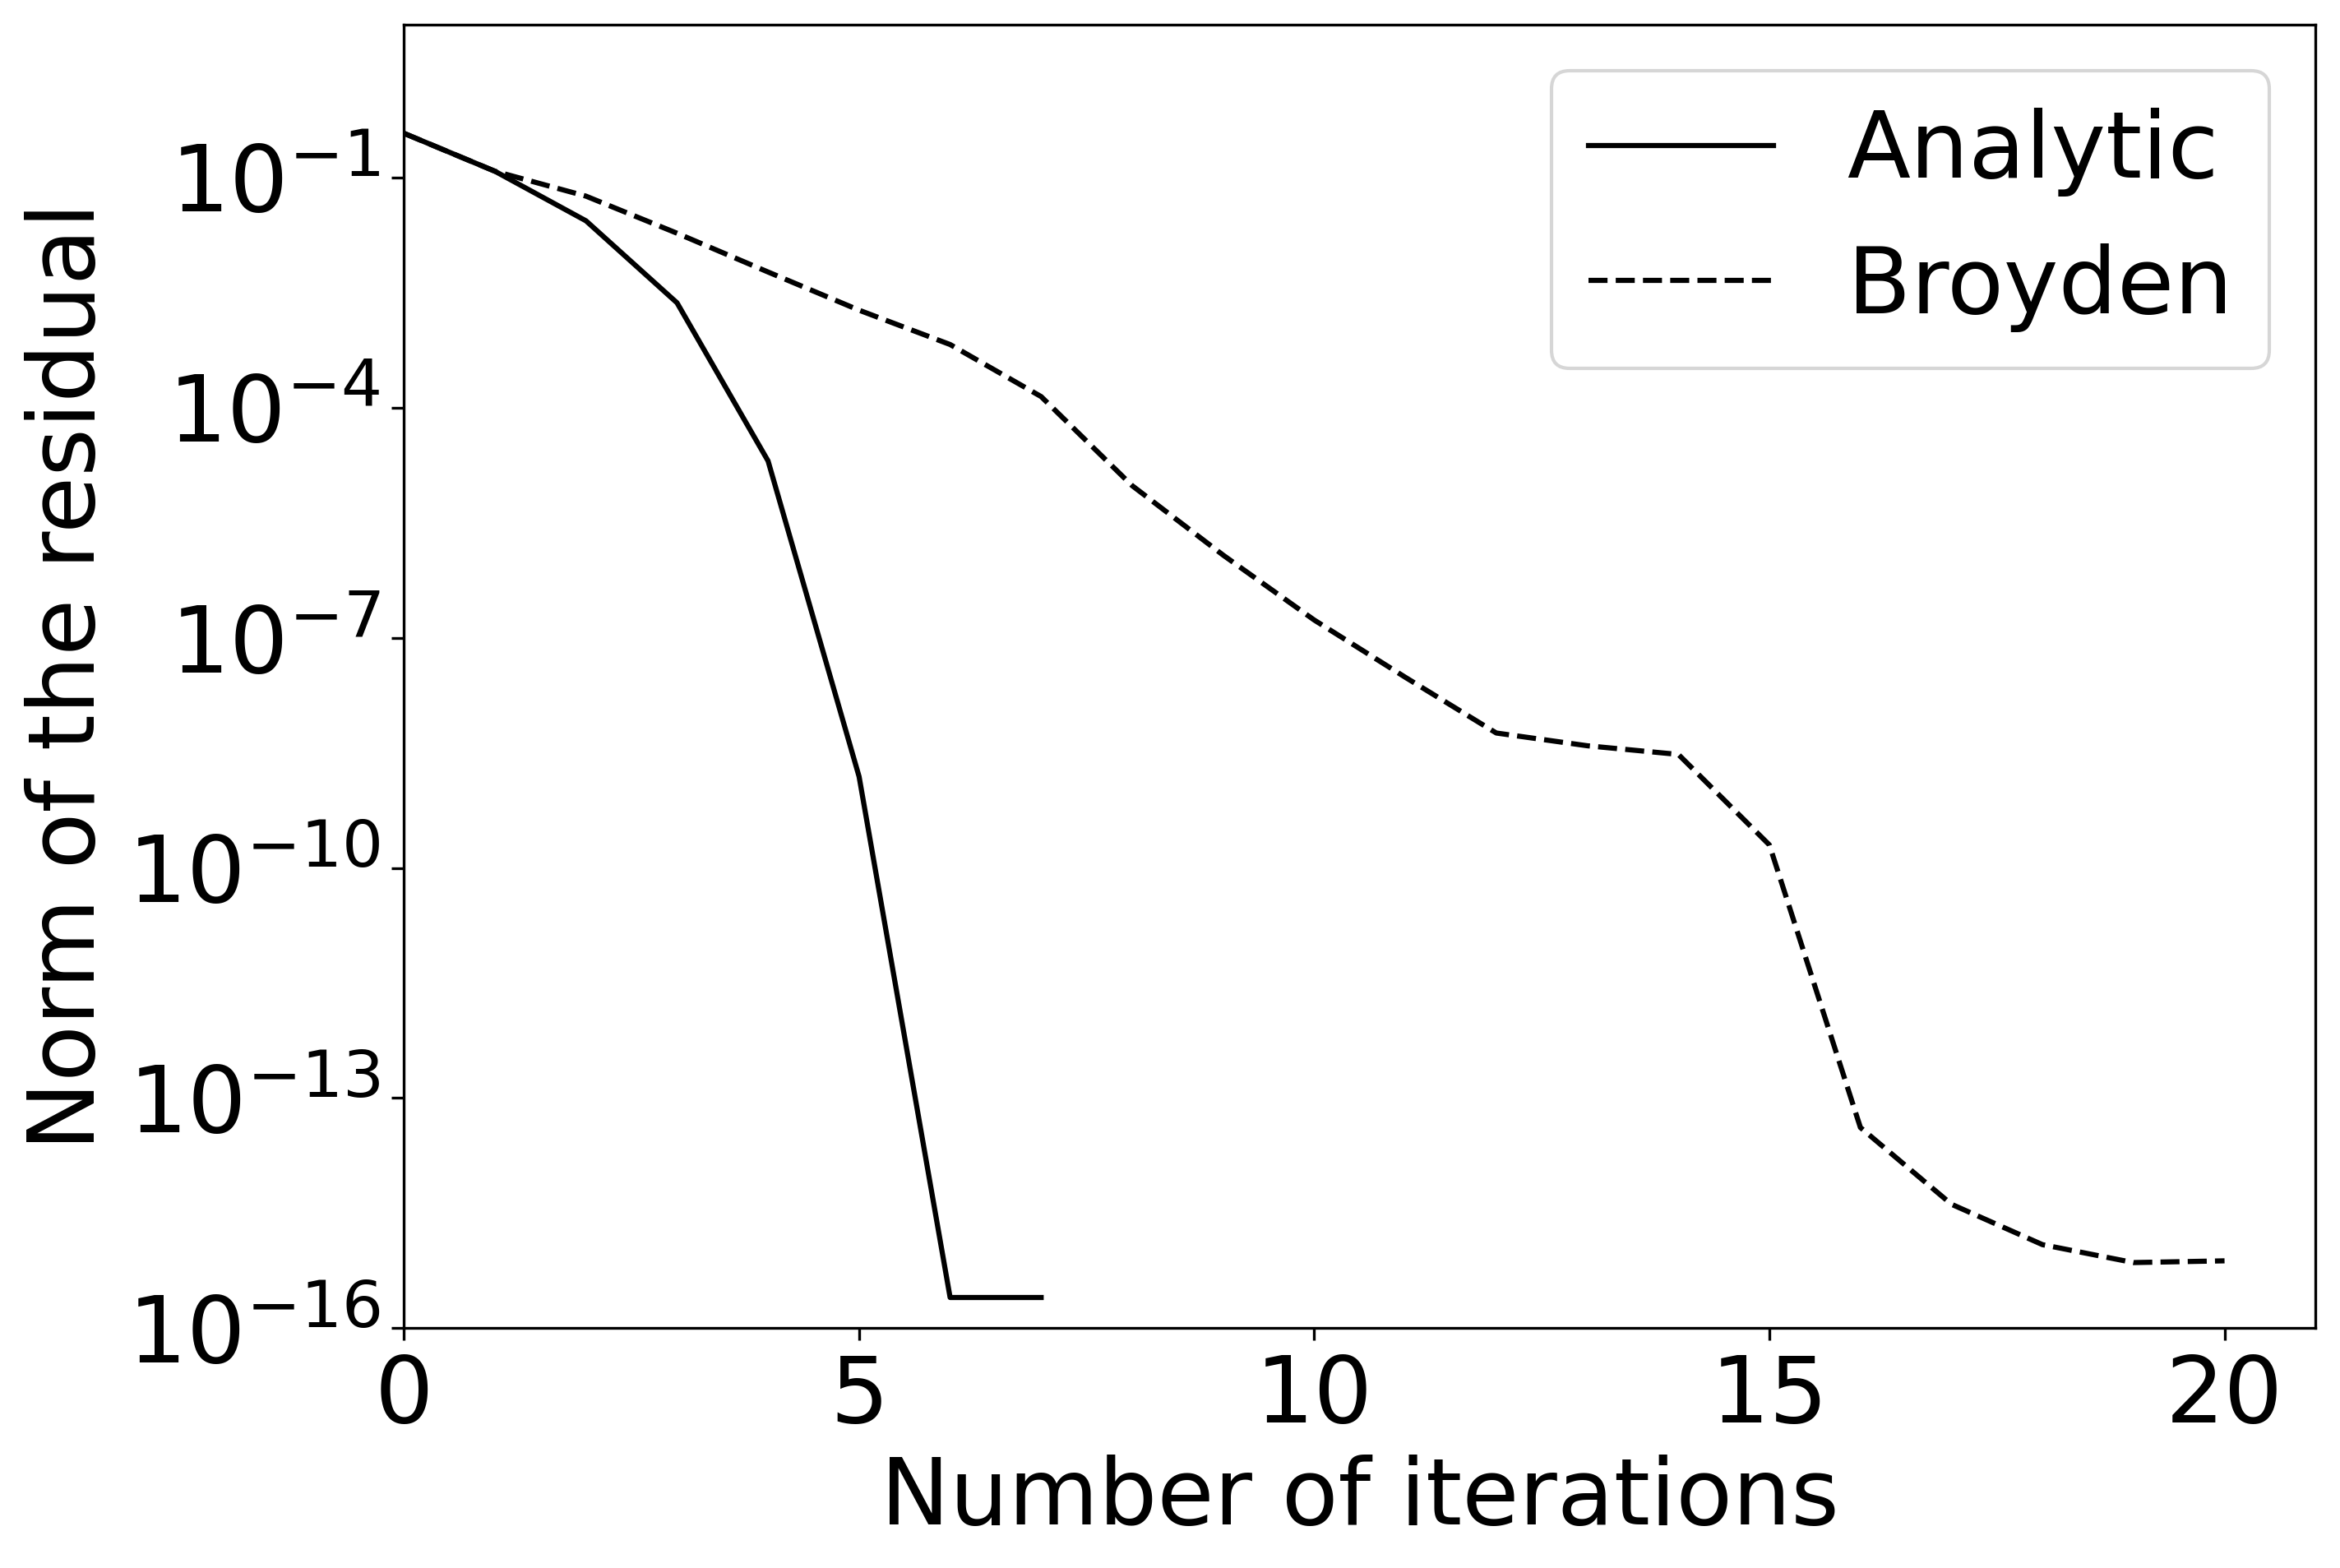
\includegraphics[width=0.9\textwidth]{images/NewtonIterationConvergence5Elements.png}
 		\subcaption{5 fault elements} 
 	\end{subfigure} 
 	\begin{subfigure}{0.32\textwidth}
 		\centering
 		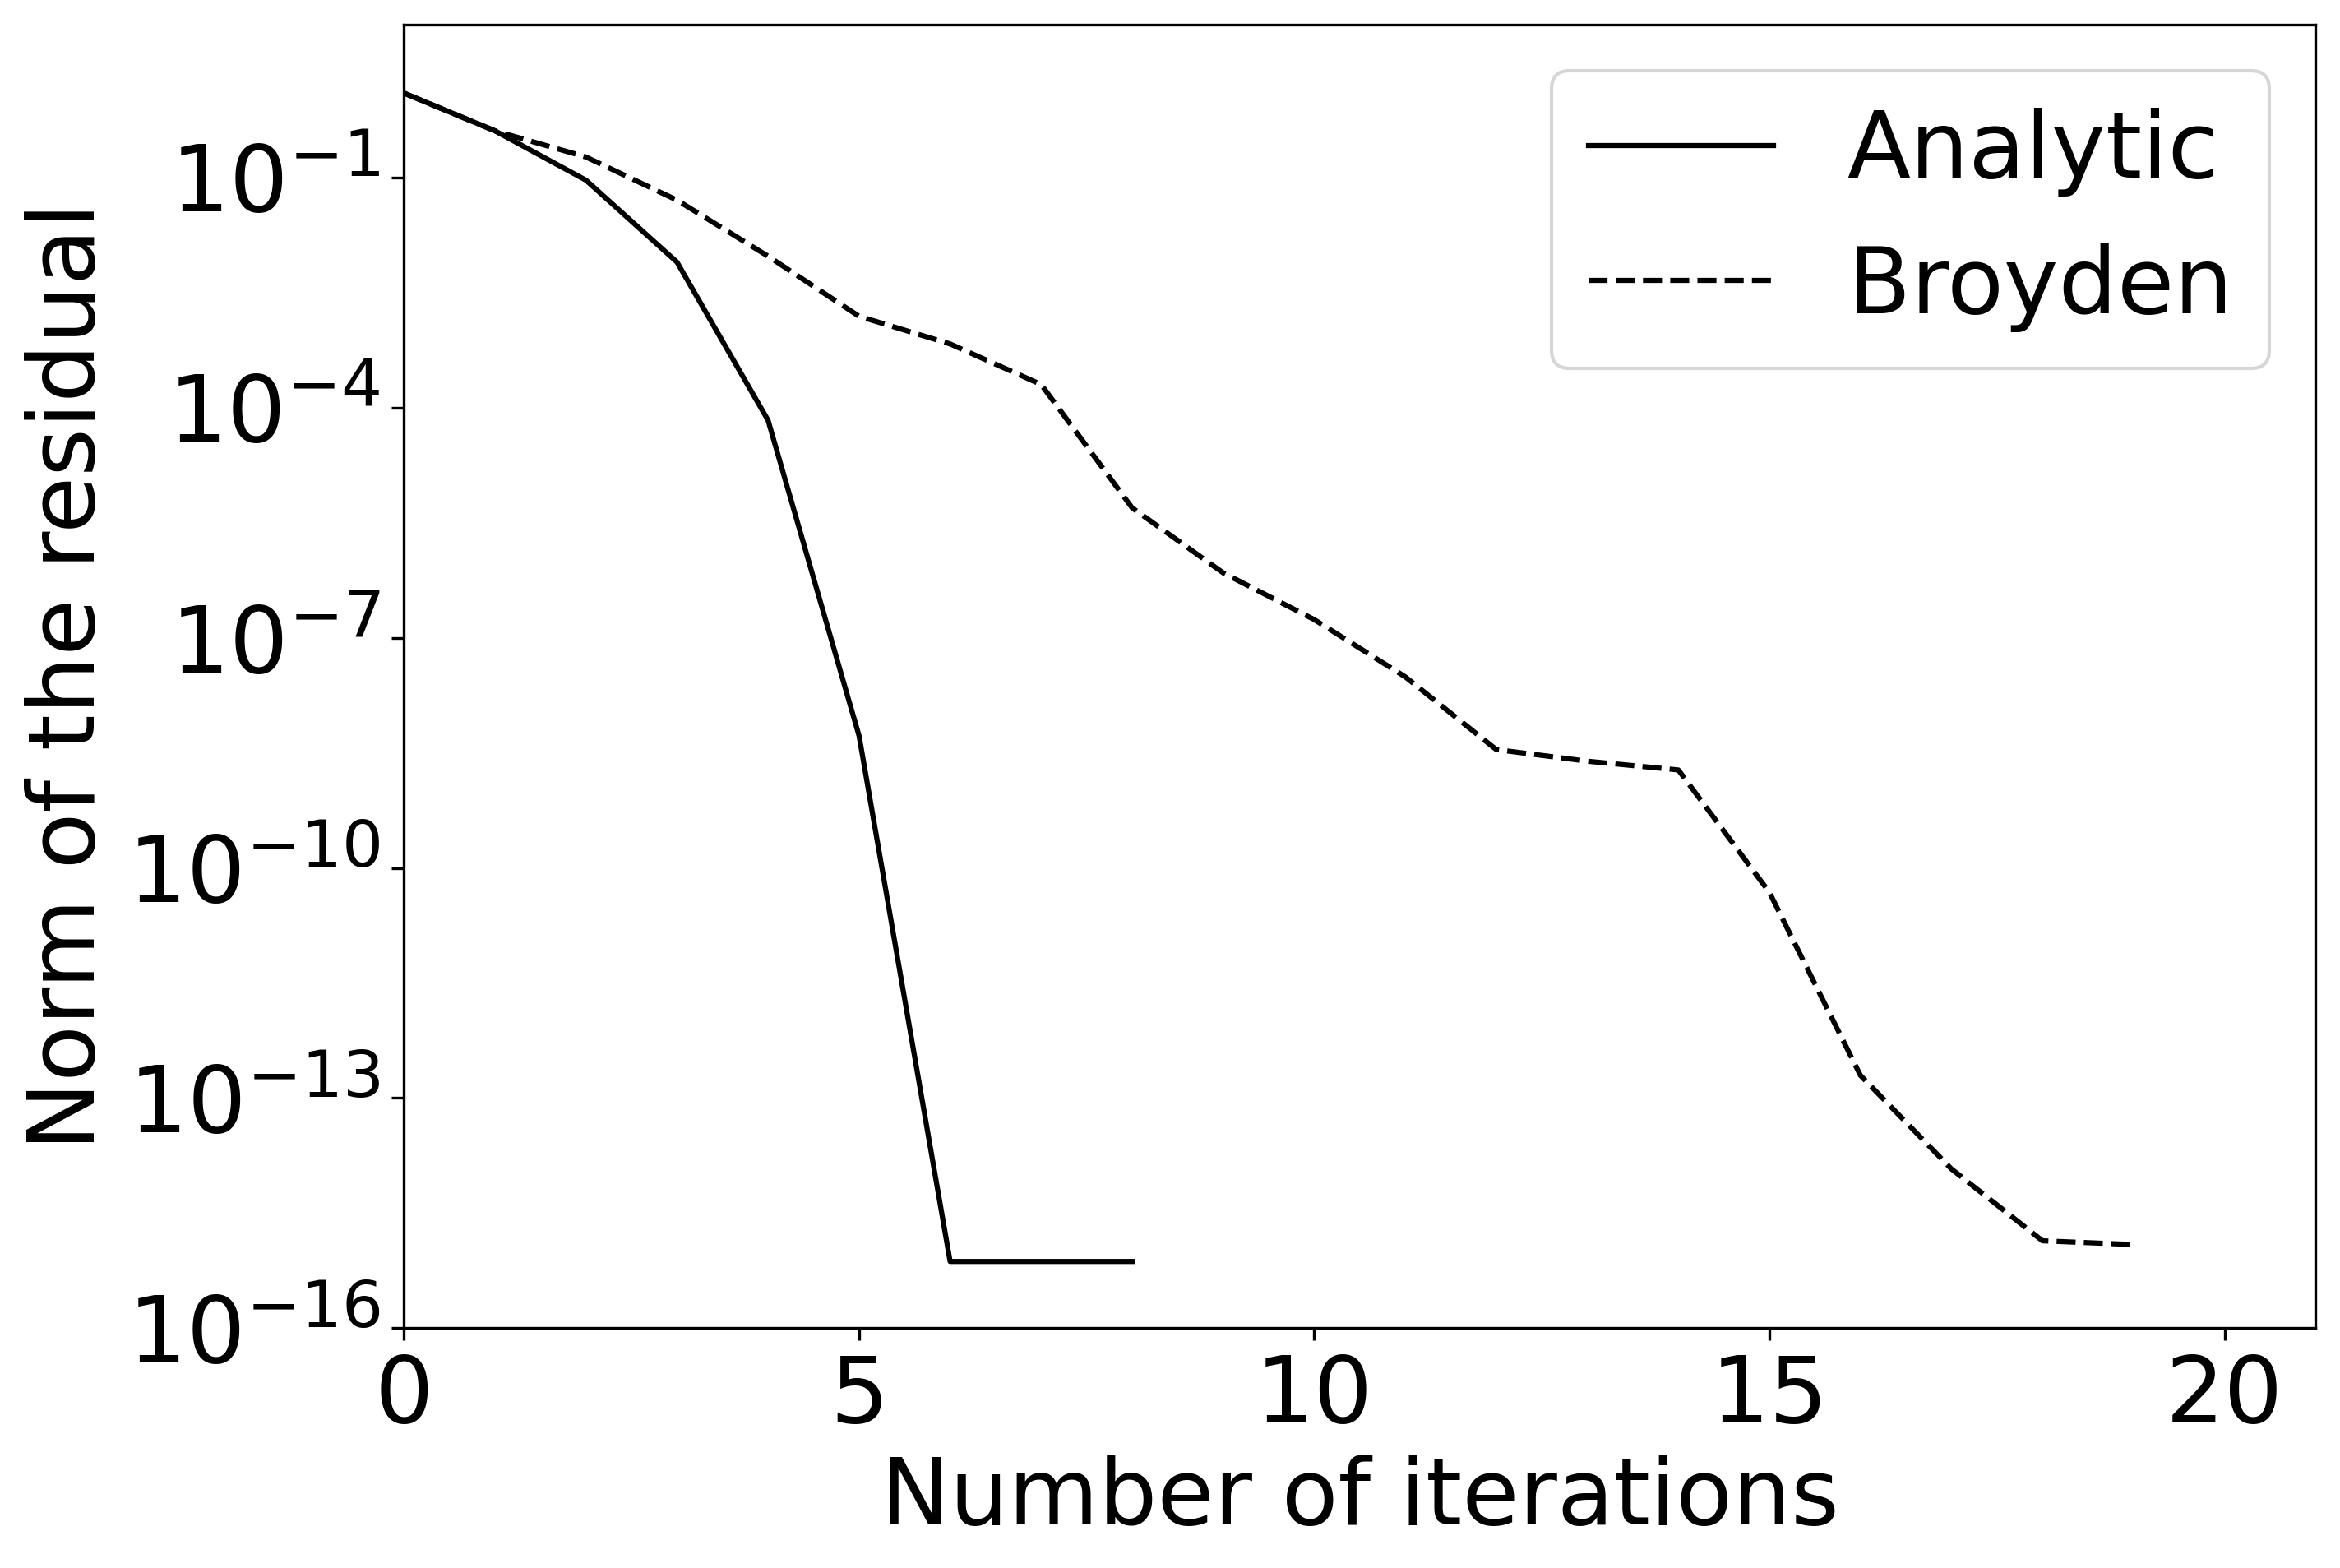
\includegraphics[width=1\textwidth]{images/NewtonIterationConvergence40Elements.png}
 		\subcaption{40 fault elements} 
 	\end{subfigure}
 	\begin{subfigure}{0.32\textwidth}
 		\centering
 		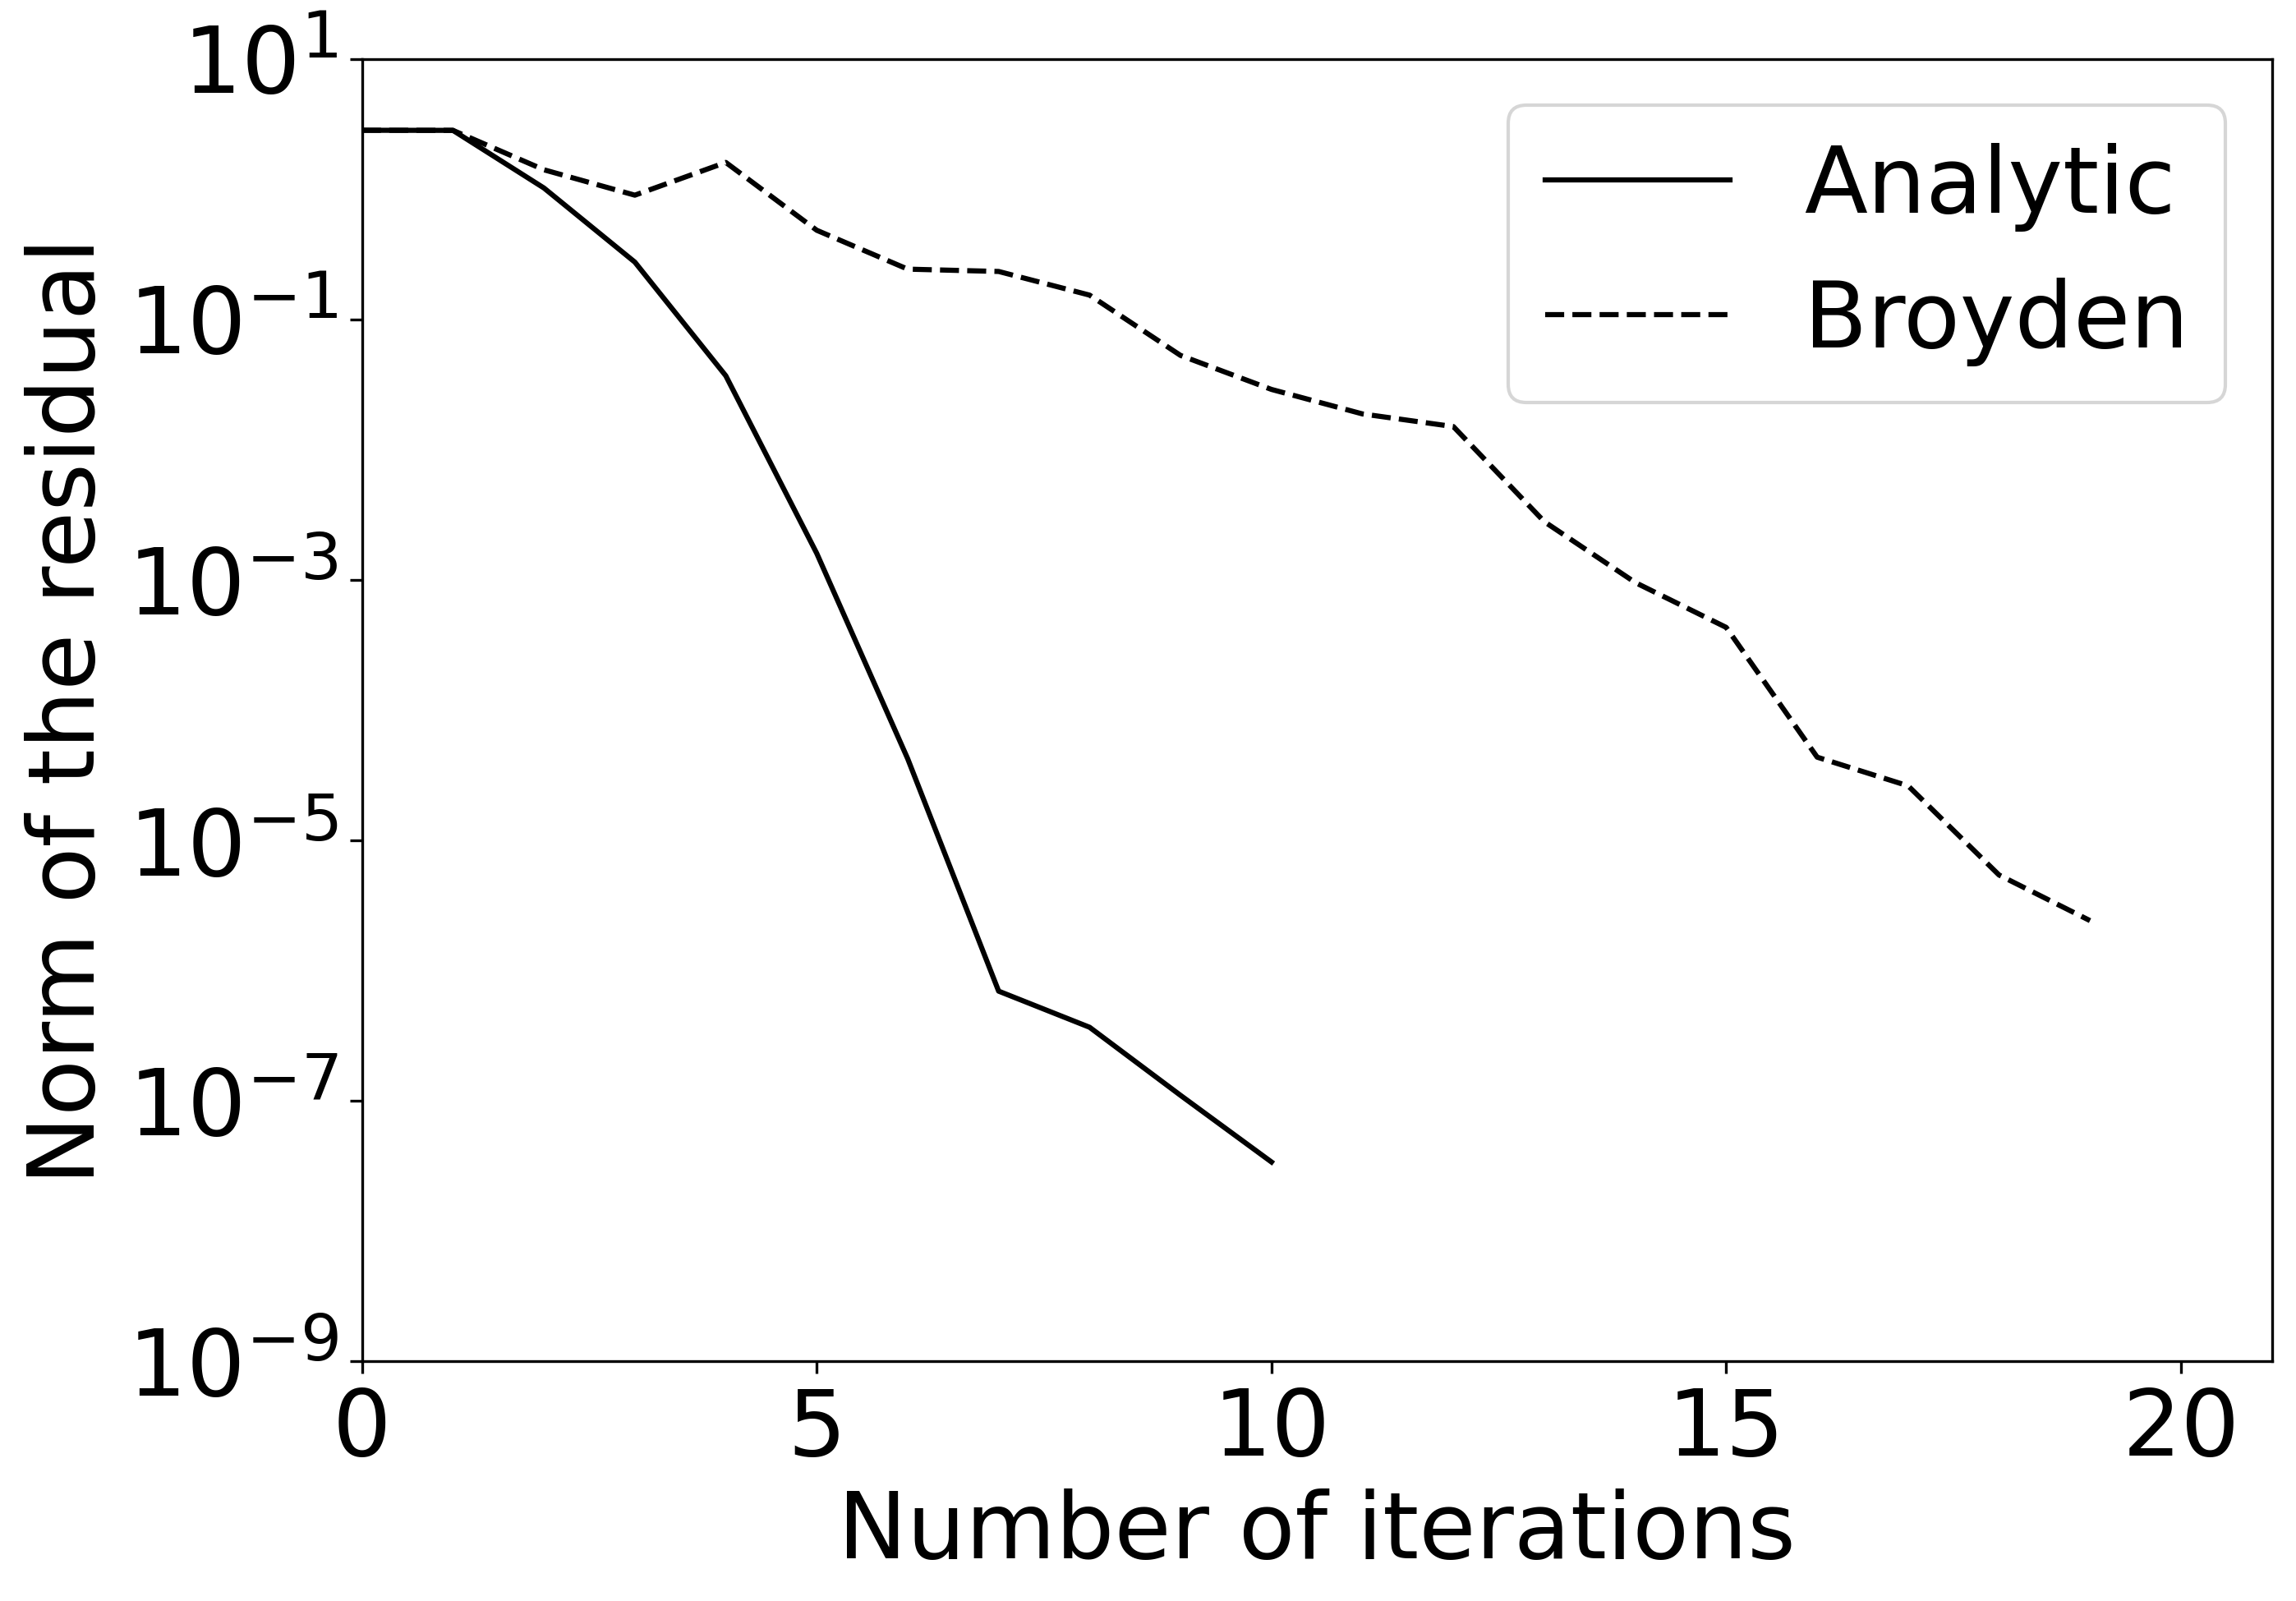
\includegraphics[width=1\textwidth]{images/NewtonIterationConvergence200Elements.png}
 		\subcaption{200 fault elements} 
 	\end{subfigure}
 	\caption{Evaluation of the L2 norm of the residual $\phi(x_n)$ at each iteration of the Newton and Broyden methods}
 	\label{fig:convergenceNewtonAndBroyden}
 \end{figure}
 It can be immediately seen that the Newton method with an analytical expression of the Jacobian reaches much faster the required tolerance of $10^{-8}$ as if it was approximated with the Broyden method. The convergence rate even seems to be quadratic, as one would expect for the Newton iteration. ???? Add some convergence test ????


\subsection{Limitations of the use of the Jacobian}
The main advantage of implicit methods over explicit methods is to allow larger time steps without loss in accuracy. The program execution is therewith expected to be accelerated. The proposed calculation of the Jacobian matrix and its application in Newton iterations comes along with some drawbacks with respect to the required calculation effort. \\
As described in \autoref{ssec:AnalyticalDerivationOfTheJacobianMatrix}, the computation of the Jacobian matrix can be split up in one constant part $\frac{\partial \tau_p}{\partial S_l}$ that has to be evaluated once at the beginning of the simulation and only depends on the domain geometry and in one variable part, that needs to be updated after each evaluation of the solution vector $x_n$. The initialization can be quite computationally expensive, at it requires, for each column of $\frac{\partial \tau_p}{\partial S_l}$, to solve the Discontinuous Galerkin system for the entire domain with the corresponding unit vector as right-hand side vector. Each calculation of this linear system is approximately as expensive as performing one time iteration with an explicit solver, since solving the same linear system is the most expensive operation of a time iteration. For large domains with several hundreds or thousands of fault elements, which each contains a couple of fault nodes, this initialization operation takes a considerable amount of time. In comparison with an explicit scheme, a potential implicit method starts the race for the fastest solver with a penalty of about $n$ explicit time iterations, where $n$ is the total number of nodes on the fault. The advantages of implicit methods will therefore only pay off after a high number of iterations and make such methods of interest only if the simulated time frame is very long. \\
Another potential drawback of the Newton method is that a linear system of size $n$ needs to be solved at each iteration step. This might still sound much less than solving for the displacement on the whole DG-domain of size $N$ as it is required to evaluate the right-hand side of the ODE at each iteration too. However, the DG system has a constant matrix $A$ whose LU-decomposition can be calculated once at the beginning of the simulation and each evaluation of the right-hand side only requires a backward substitution of complexity $\mathcal{O}\left(N^2\right)$. For the Jacobi matrix, such a pre.processing is not available since it changes along with the solution vector. Every calculation to solve the linear system in the Newton iteration is achieved with a complexity of the order $\mathcal{O}\left(n^3\right)$. In particular in large domains with many fault nodes the solver with cubic complexity may involve a substantially higher execution time than the one with quadratic complexity. Notwithstanding, for such large domains, the question has to be asked whether a direct solver is still appropriate or whether iterative solvers yield acceptable results. Such considerations are however beyond the scope of this thesis (so far ???).

\section{Second Order Differential Equation}
So far, the original problem in \autoref{ssec:physicalDescriptionSEAS2D} has been formulated as a first order ODE in \autoref{eq:ODE_formulation_SEAS}, in which the friction law is solved implicitly within each evaluation of the right-hand side, such that explicit time integrators can be used. The solution vector has a compact size and only includes the slip $S$ and the state variable $\psi$. Alternatively, the problem can be directly formulated as a DAE, where the solution vector is extended by the slip rate $V$, such that it can be solved through the friction law iteratively together with the time quantities $S$ and $\psi$. A compact form of the DAE has also been formulated, where the derivative slip rate is directly used in the friction law instead of introducing a new variable $V$. \\
The original motivation was to define an extended ODE formulation as counterpart to the extended DAE form, such that the solution vector contains an additional component for the slip rate $V$. To achieve this goal, it is necessary to find a function $h(t,S,\psi,V)$ which describes the change in time of the slip rate $\frac{dV}{dt}$. Since $V$ itself is the time derivative of the slip, this function $h()$ corresponds to the second time derivative of the slip, or the slip acceleration. The new ODE formulation is: 
\begin{align}
&&	 x      =& \begin{pmatrix}	S                     \\ \psi           \end{pmatrix}      &
	 		   \begin{pmatrix}	\ddot{S}              \\ \dot{\psi}     \end{pmatrix}
			=& \begin{pmatrix}	h(t,S,\psi,\dot{S})   \\ g(\psi, V)     \end{pmatrix}
			 	 		 \\ &\Leftrightarrow&	 		  		 
	 x      =& \begin{pmatrix}	S       \\ \psi       \\ V	            \end{pmatrix}      &
   	\dot{x}  = \begin{pmatrix}	\dot{S} \\ \dot{\psi} \\ \dot{V}        \end{pmatrix}
	 		=& \begin{pmatrix}	 V      \\ g(\psi, V) \\ h(t,S,\psi,V)  \end{pmatrix}
	 		 = F	
\end{align}
Here, the friction law does not appear in the right-hand side anymore and is implicitly included in the function $h()$. Unlike the previous ODE formulation, it does not require anymore to solve the friction law implicitly at every time step for the slip rate $V$ (or any other quantity), therefore, the new formulation is in some sense a "true" ODE and not a hidden DAE anymore. Another very beneficial advantage is, that if the boundary conditions of the DG domain are linear in time, it does not require to solve the DG system at every time step anymore, which is the main performance bottleneck after initialization in the first order formulations. 

\subsection{Derivation of the second order ODE}
This section will focus on the derivation of the right-hand side function $h(t,S,\psi,V)$, which is necessary to formulate the second order ODE. Starting point is the expression for the friction law in \autoref{eq:SEASDAE_frictionLaw}. At any time in the simulation, this algebraic equation always evaluates to zero, and therefore, its time derivative is also equal to 0. With the help of the formula of total derivatives, we obtain following expansions: 
\begin{align}
	0 = \dv{f}{t} &= \pdv{f}{t} + \pdv{f}{S}\dv{S}{t} + \pdv{f}{\psi}\dv{\psi}{t} +  \pdv{f}{V}\dv{V}{t} \\
					  &= \pdv{f}{t} + \pdv{f}{S}V + \pdv{f}{\psi}g(\psi,V) + \pdv{f}{V}h(t,S,\psi,V)
\end{align}
The partial derivatives of $f$ that occur are calculated in the same way as for the Jacobian matrices of the first order formulations. The terms $\pdv{f}{\psi}$ and $\pdv{f}{V}$ are diagonal matrices with the entries stated in \autoref{eq:partial_df_dpsi} and \autoref{eq:partial_df_dV} and the term $\pdv{f}{S}$ is a constant, full matrix which depends on the geometry of the domain and is derived in \autoref{eq:partialDerivative_df_dS}. After some transformations, the function $h()$ can be expressed as: 
\begin{equation}
	h(t,S,\psi,V) = -\left(\pdv{f}{V}\right)^{-1}\left(\pdv{f}{t} + \pdv{f}{S}V + \pdv{f}{\psi}g(\psi,V)\right)
\end{equation}
It can be noted that this expression is very similar to the Jacobian matrix of the first order ODE formulation. If $x=(S,\psi)^T$ stands for its solution vector and $\mathbf{J}_{S}$ denotes the first row of block matrices of its Jacobian matrix in \autoref{eq:Jacobian_ODE_formulation}, an alternative definition of $h()$ could be: 
\begin{equation}
	h(t,S,\psi,V) = \mathbf{J}_{S}\dv{x}{t} -\left(\pdv{f}{V}\right)^{-1}\pdv{f}{t}
\end{equation}
The last missing term is the partial derivative of the friction law $f$ with respect to the time variable $t$. In its definition, the only component that directly depends on time is the traction $\tau$ through the boundary conditions of the DG domain. Typically, at boundary nodes which are not on the seismic fault, the slip $S_b$ there is prescribed and evolves with time to represent the natural movement of the tectonic plate. For a constant environment slip rate $V_p$, we calculate $S_b=V_pt$ for the general case or $S_b=V_p/2\;t$ if the domain is symmetric. The boundary slip is linear in time, so its first derivative $\dot{S}_b$ will be constant. In the DG formulation, boundary conditions are included in the term $f_q$ of \autoref{eq:???}, and are added to the traction $\tau$ on the fault only after linear transformations. To obtain $\pdv{\tau}{t}$ on the fault, it is then sufficient to solve the Poisson problem with only $\dot{S}_b$. Since this term is constant, $\pdv{f}{t}$ is also constant it is enough to solve the Poisson problem once at the beginning of the simulation and then, at each evaluation of the right-hand side of the ODE, use the same term $\pdv{f}{t}$. To reuse existent code structures, $\pdv{\tau}{t}$ can be pre-calculated with the DG solver for $\tau$ using a slip of 0 everywhere on the fault and by evaluating the boundary condition at the time $t=1$. \\
In comparison with the first order ODE formulation, the new second order formulation needs a considerable initialization phase, but evaluates the right-hand side of the ODE much faster. In addition of the LU-decomposition of the DG matrix $A$, the initialization of the Jacobian $\pdv{f}{S}$ needs to solve the Poisson problem on the DG domain of size $N$ once per fault node, so in total $n$ times. Moreover, the problem needs to be solved once to calculate the initial condition of $V$ from the initial $S$ and $\psi$ and once to initialize the time derivative of the friction law $\pdv{f}{t}$. At each evaluation of the right-hand side of the first order ODE, the DG system needs to be solved with its LU-decomposition in $\mathcal{O}\left(N^2\right)$ and the remaining components of the vector set up in $\mathcal{O}\left(n^2\right)$ because of the matrix-vector product in $\tau$, so the total complexity is $\mathcal{O}\left(n^2+N^2\right)$. In contrast, the second order formulation only needs matrix-vector multiplications on the fault node, so its total complexity per evaluation is reduced to $\mathcal{O}\left(n^2\right)$. Since $n\ll N$, it is expected that the new formulation performs much better for long simulation times. \\
However, if the boundary conditions are not linear in time, their derivation is not constant in time anymore and needs to be evaluated at every time step, and therefore the solution of the Poisson problem is needed again at every time step. The complexity increases back to $\mathcal{O}\left(n^2+N^2\right)$ and the main advantage of the second order formulation is lost. For now, we do not consider this case and always assume that the boundary conditions are linear in time.  \\
\autoref{fig:timeEvolution_2ndOrderODE_vs_1stOrderODE} shows the maximum slip rate that occurs throughout the simulation time for both ODE formulations. Both curves overlap well, at least up to 1000 years of simulation time, so it proves that the new approach leads to the same results. This graph also indicates at which times earthquakes happen: after two initial earthquakes, a regular pattern of three close earthquakes alternates with one singular earthquake every 90 years approximately.
\begin{figure}[H]
	\centering
	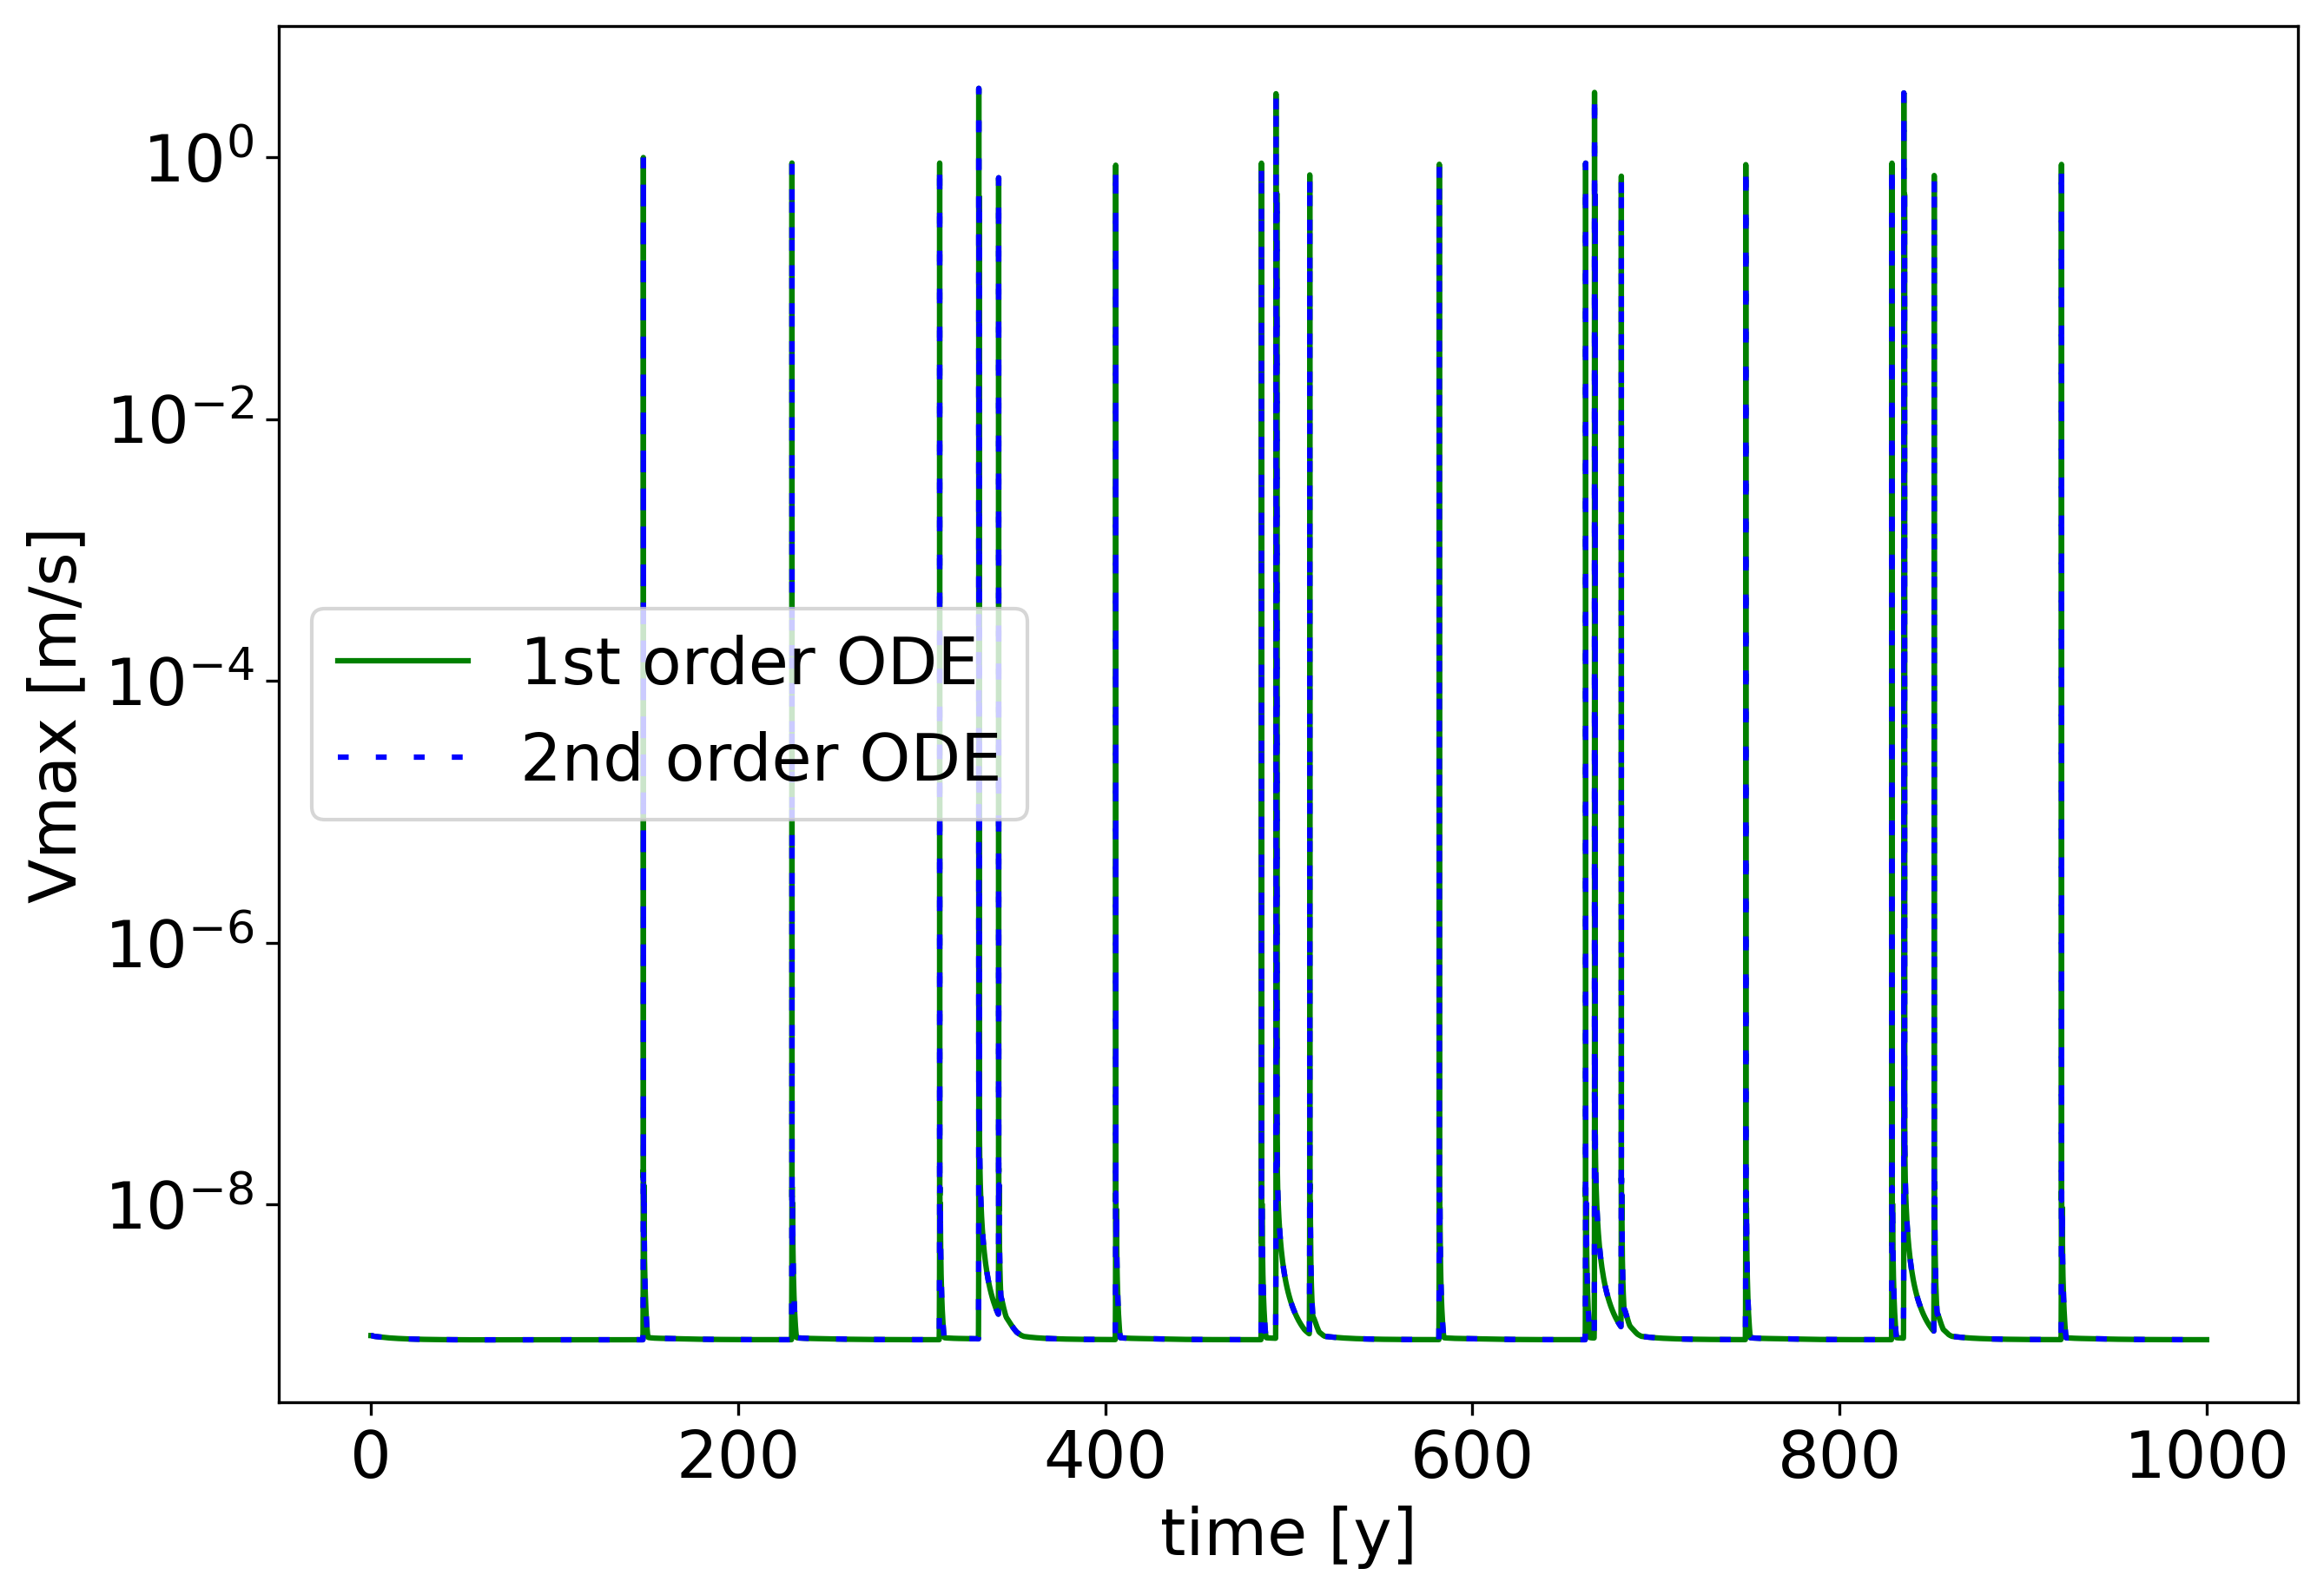
\includegraphics[width=0.45\textwidth]{images/TANDEMtimeEvolutionVExtendedODE1stvs2ndOrder.png}
	\caption{Maximum slip rate in the 1st and 2nd order formulations on a domain with 5 fault elements for 1000 years} 
	\label{fig:timeEvolution_2ndOrderODE_vs_1stOrderODE}
\end{figure}

\subsection{Derivation of the analytic Jacobian}
This will be tricky, involves Hessian matrices and stuff of the friction law. --> next thing to implement

\subsection{Error estimation}
Despite the lack of an analytic solution to the problem, this formulation of the problem offers a very powerful tool to evaluate the accuracy of the results. Since the slip rate is not calculated from the friction law anymore, it is not ensured that it is always equal to 0 up to numerical precision, as it was the case in the first order formulations of the SEAS problem. We could then evaluate the friction law at every timestep to assess the accuracy of the numerical integration. A large deviation from 0 of the absolute value of the friction law at a given timestep means that the integrator provides poor results. For a standard execution of the simulation with the second order formulation, this metric is not available, since the evaluation of $\tau$ in the friction law requires to solve the Poisson problem, and the big advantage of the new formulation is exactly not to solve this system. For the following graphs, The value of the friction law has been exceptionally calculated. \\

For the first set of pictures, a very small domain with 5 fault elements has been chosen to be able to observe the evolution of the quantities over a long period of time. The tolerances for the slip and the state variable have been fixed to $10^{-7}$. \autoref{fig:timeEvolution_2ndOrderODE_differentTolerances} shows the maximum value of the friction law for varying relative relative tolerances for $V$, and the absolute tolerance is fixed to 0. From the initial condition, the slip rate is calculated to fulfill the friction law up to numerical precision, at about $10^{-15}$. After some time steps, this high precision is lost, and at every earthquake event, the difference increases sharply. Overall, the logarithmic shape of the curves indicate a linear decrease of accuracy with time, It seems that, at every evaluation of the right-hand side function, for one given tolerance of $V$, a certain local truncation error is added to the residual of the friction law. At an earthquake, much more timesteps are required and the sum of the local truncation errors sum up to form an apparent sharp increase in the global error. For lower tolerances in $V$, the increase of the error at every evaluation is smaller the accuracy is higher. This hypothesis is confirmed by \autoref{fig:timeEvolution_LTE_2ndOrderODE_differentTolerances}, which shows the absolute change of the friction law per timestep. It can be considered somehow as an estimate for the local truncation error (LTE), as it describes how the error increases at each step. For a given tolerance in the slip rate, an upper bound for the LTE can be observed. During the earthquake, the LTE is actually much lower than in the aseismic slip. Only the high number of steps required for this event result in the apparent sharp increase of the total error. 

\begin{figure}[H]
	\centering
	\begin{subfigure}{0.45\textwidth}
		\centering
		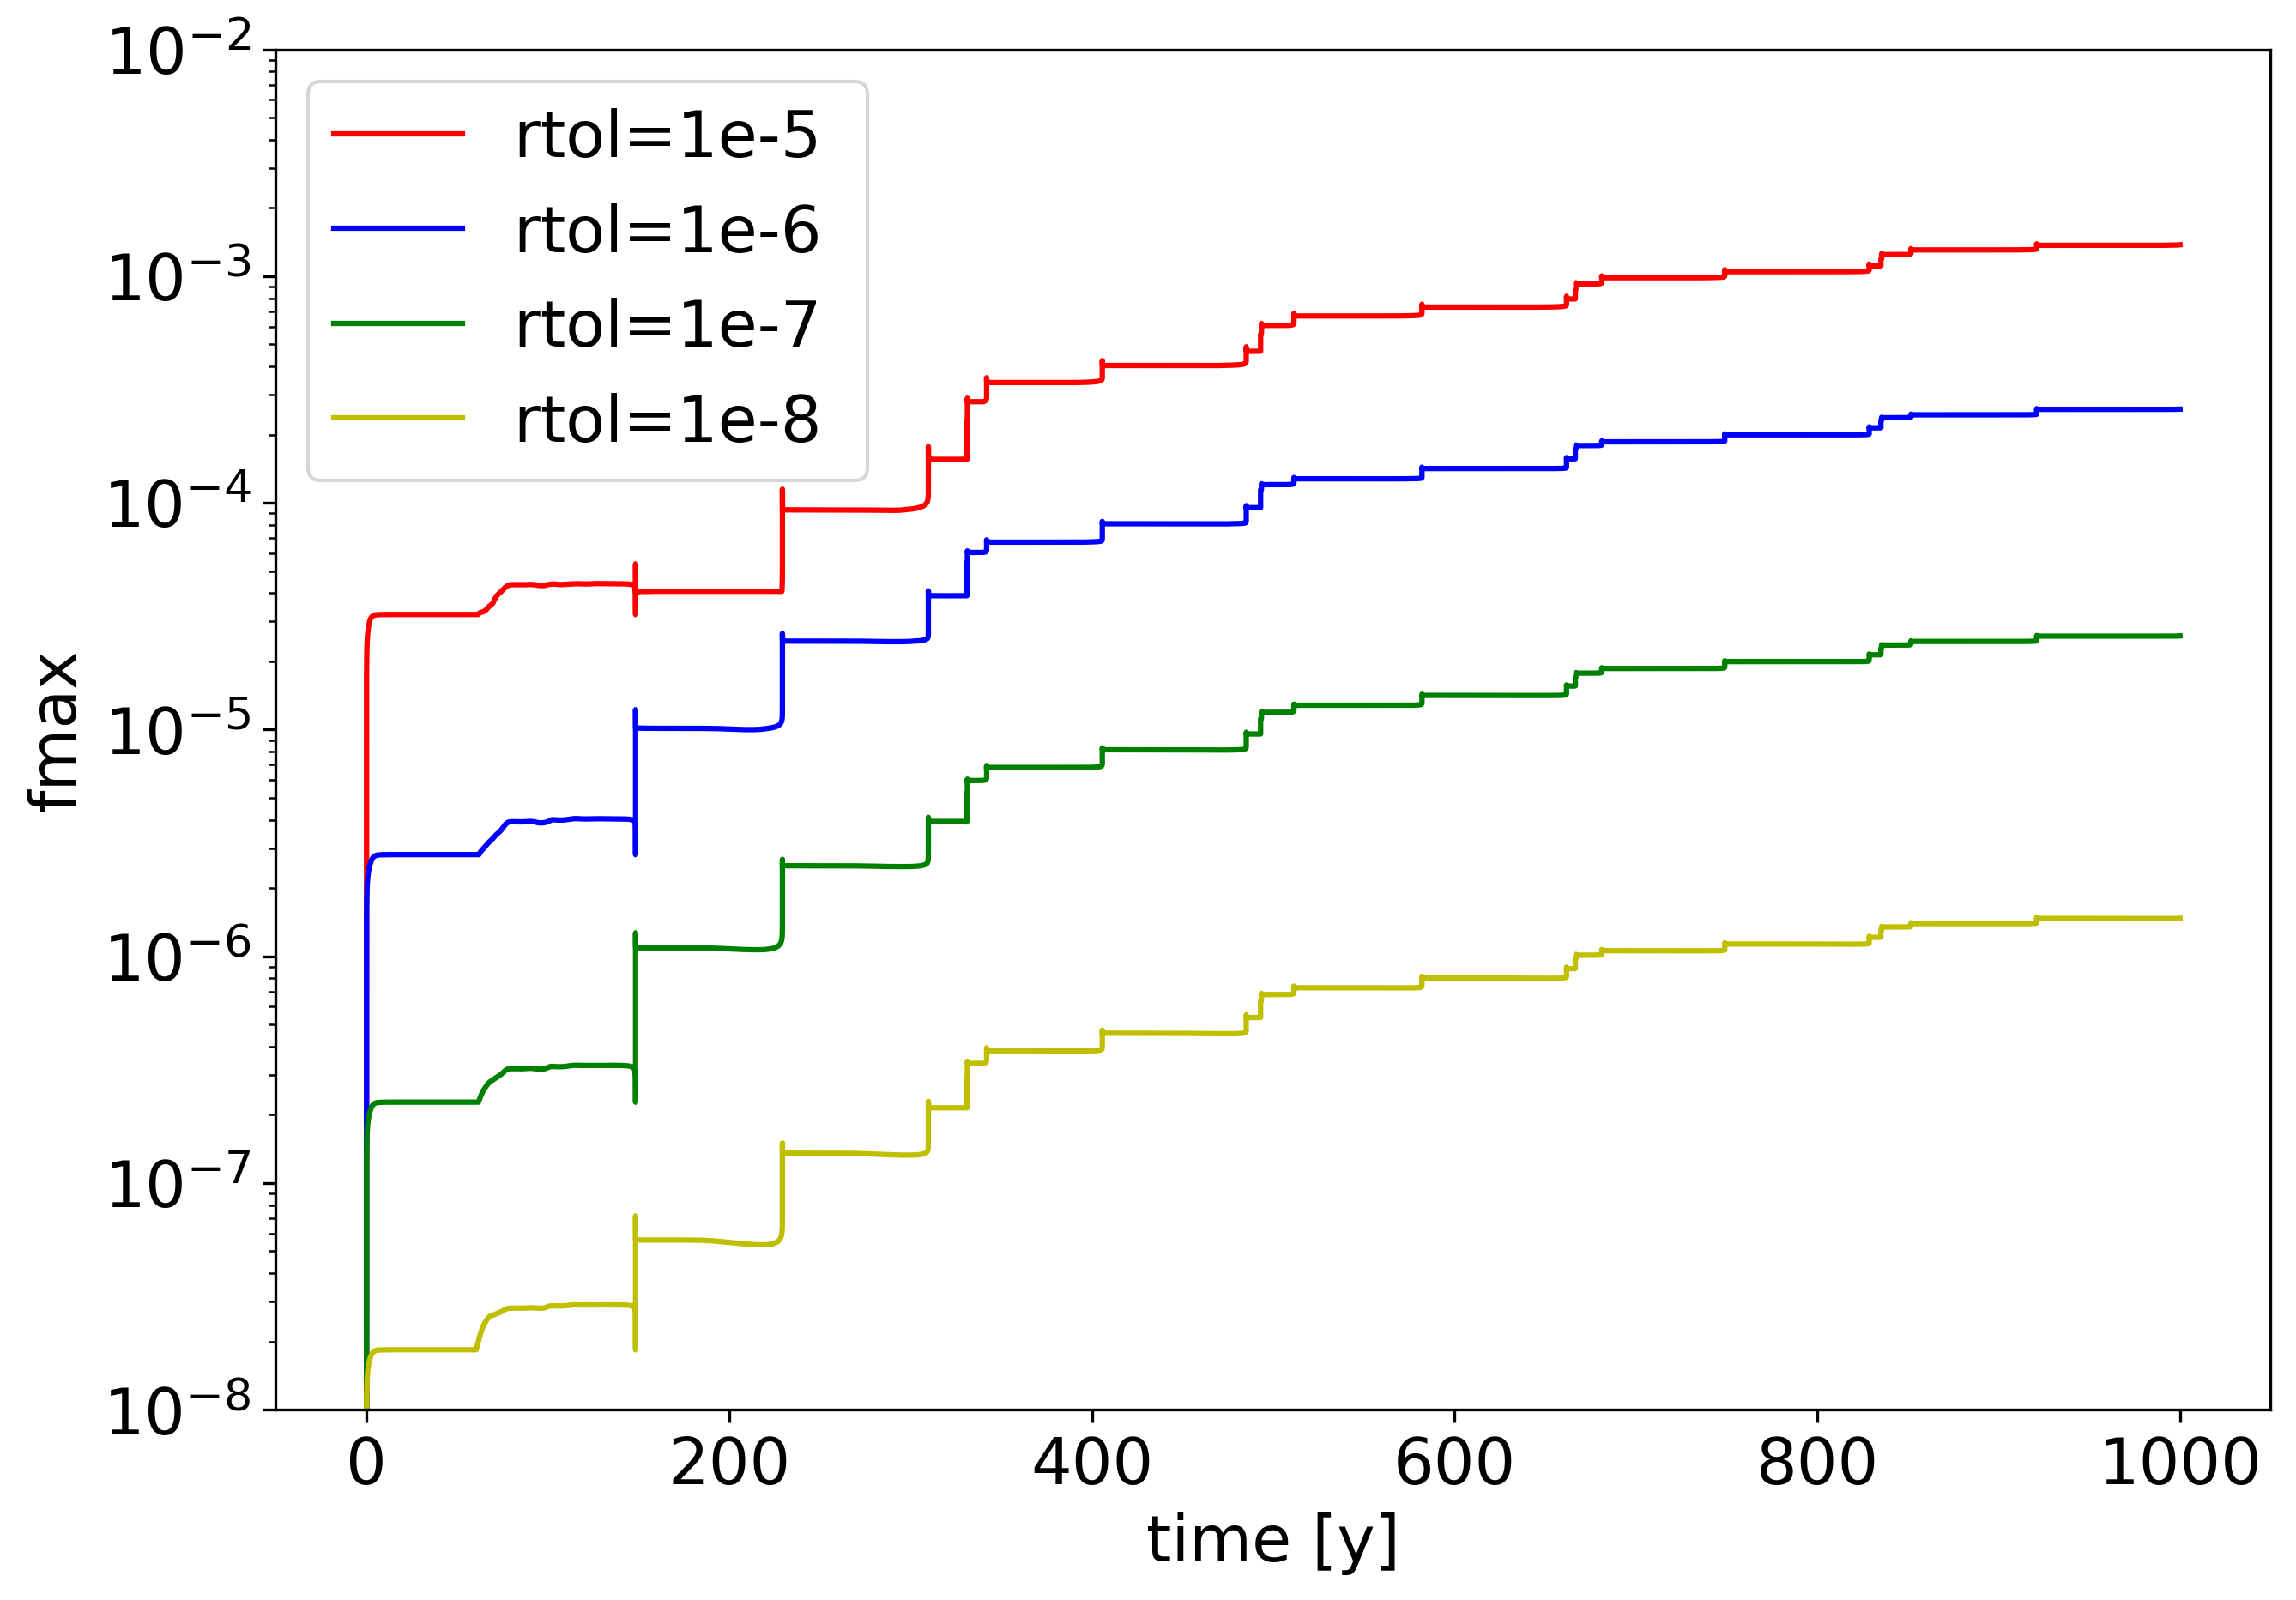
\includegraphics[width=1\textwidth]{images/TANDEMtimeEvolutionFExtendedODEDifferentTolerances.png}
		\subcaption{Maximum absolute value of the friction law} 
		\label{fig:timeEvolution_2ndOrderODE_differentTolerances}
	\end{subfigure}
	\begin{subfigure}{0.45\textwidth}
		\centering
		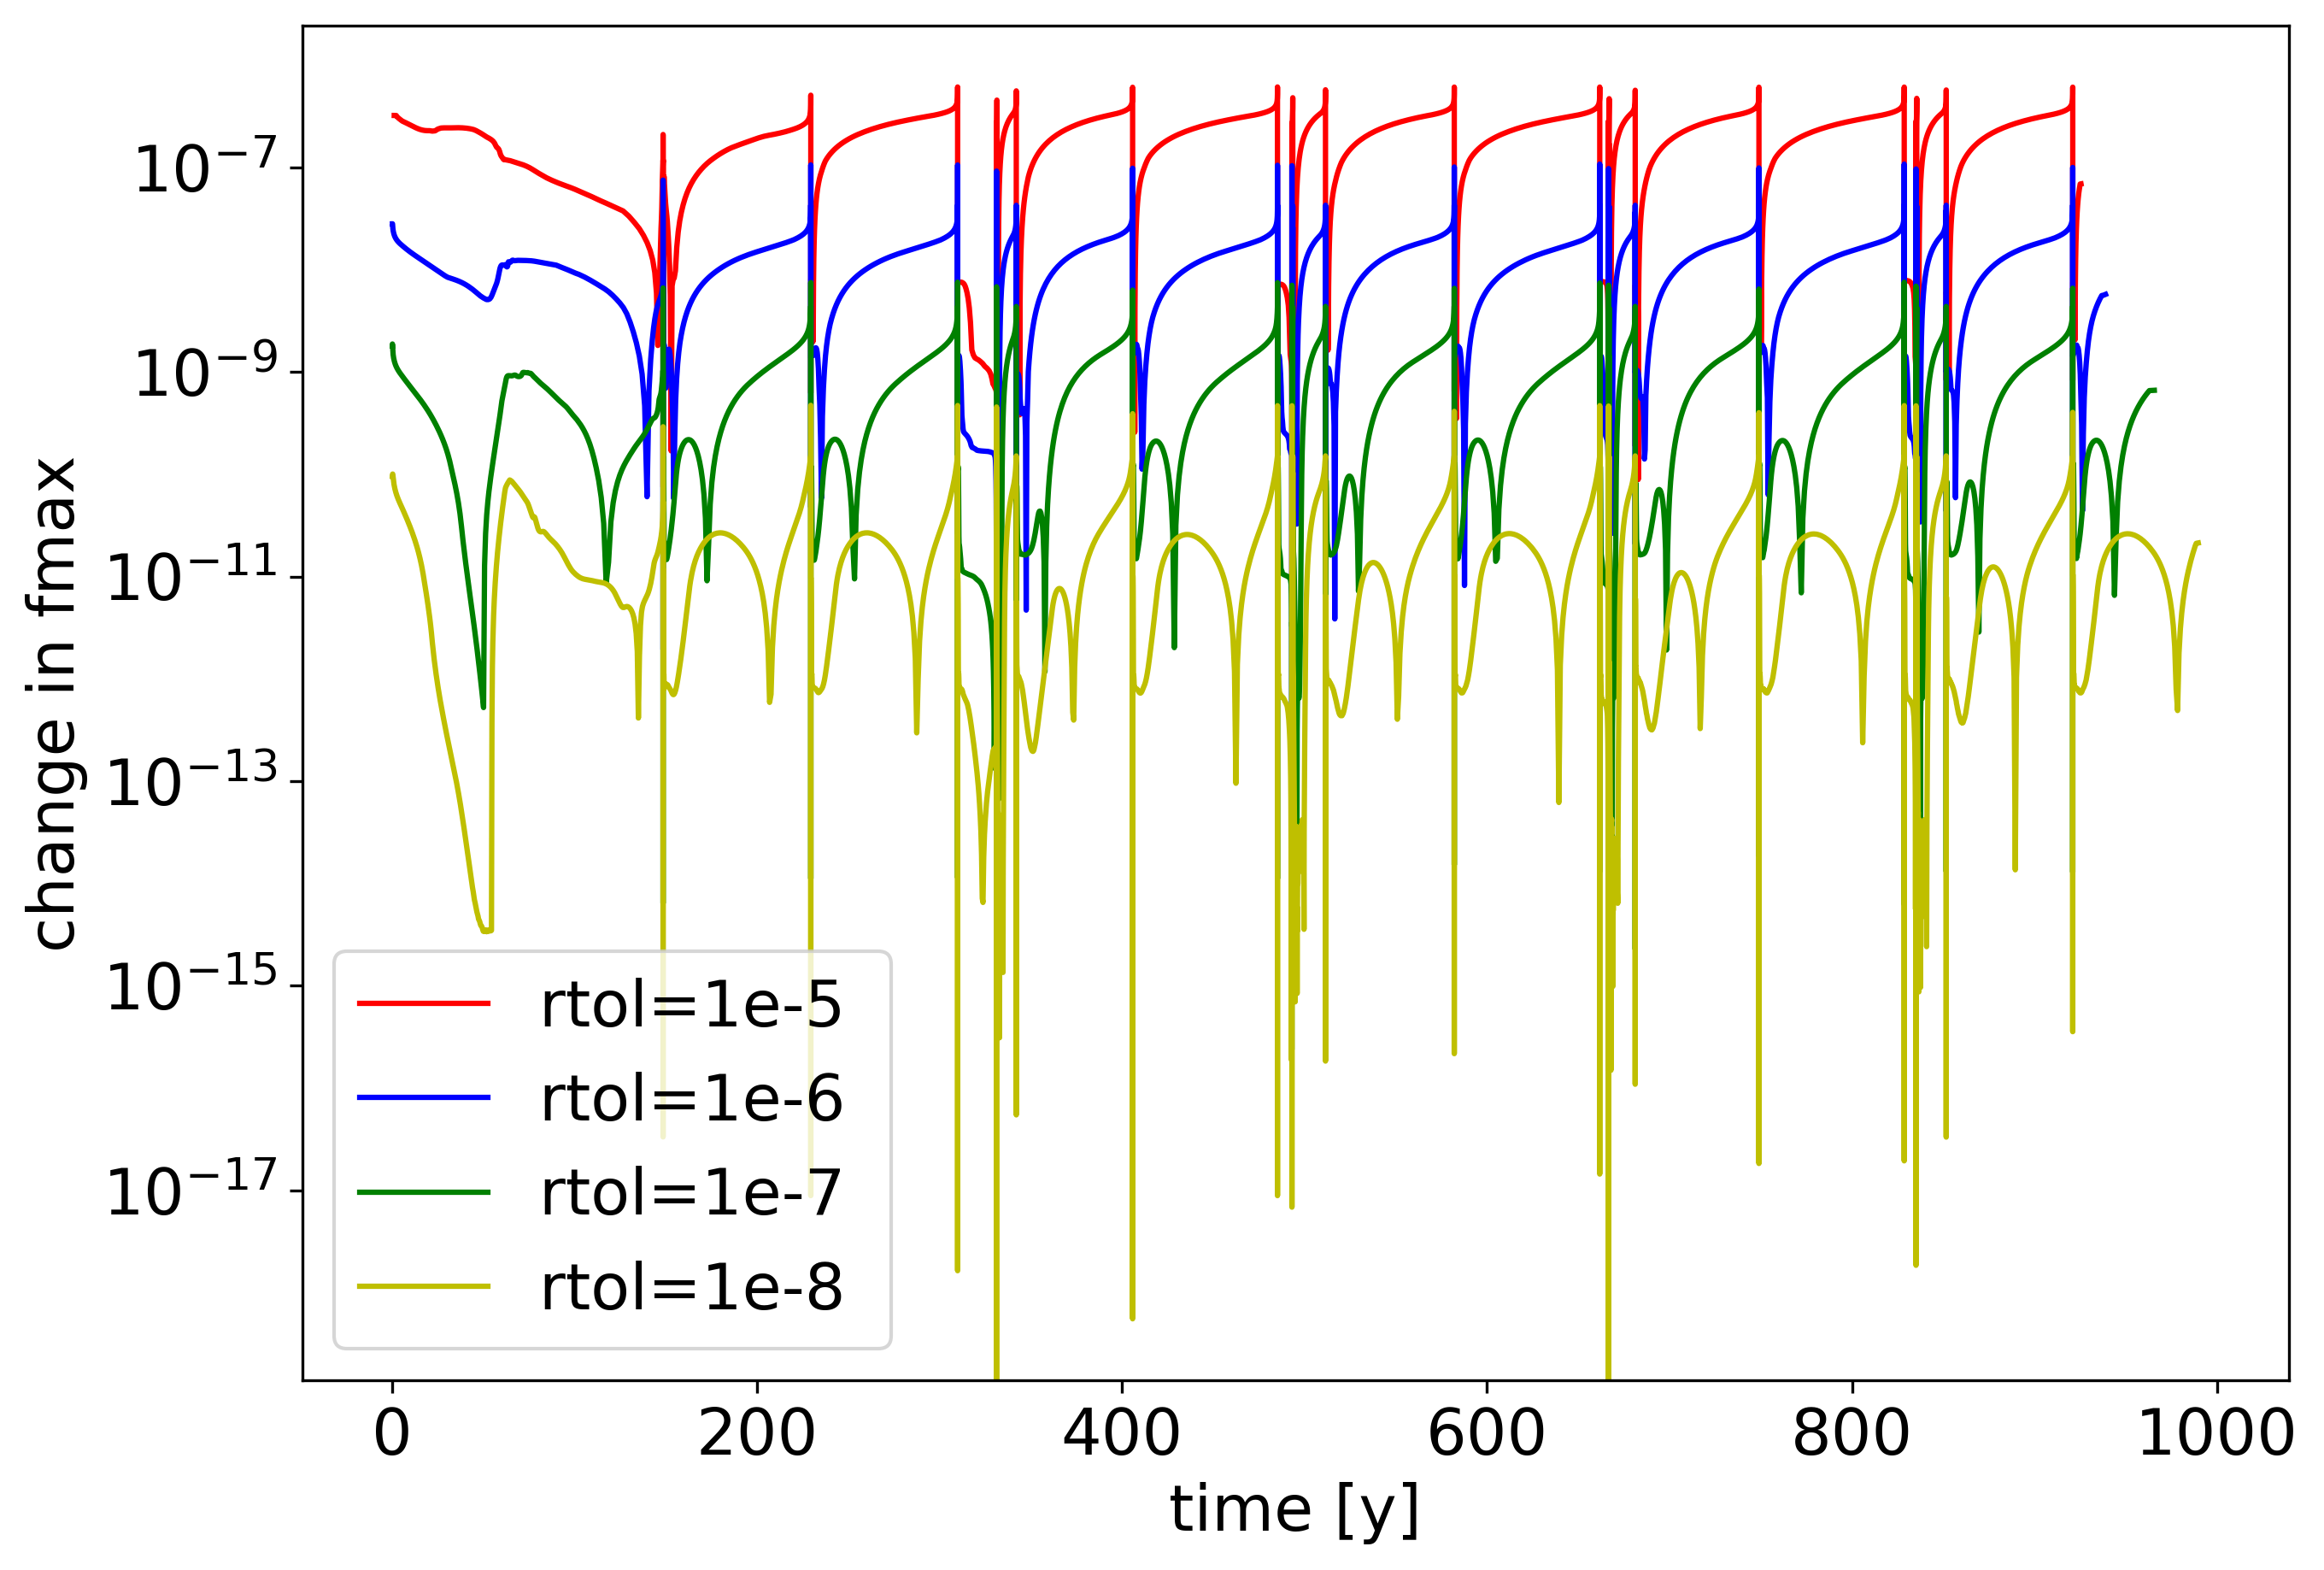
\includegraphics[width=1\textwidth]{images/TANDEMtimeEvolutionFLTEExtendedODEDifferentTolerances.png}
		\subcaption{Absolute change of the friciton law per timestep, averaged over 50 timesteps} 
		\label{fig:timeEvolution_LTE_2ndOrderODE_differentTolerances}
	\end{subfigure}
	\caption{Evolution of the value of the friction law of the 2nd order formulation with 5 elements on the fault over 1000 years with varying relative tolerances in the slip rate $V$}
\end{figure}

The local truncation error seems to depend linearly on the tolerance for the slip rate, and a similar dependency is to be expected with respect to the tolerances of the slip $S$ and $\psi$, since these quantities are also required to evaluate the friction law. Next, we investigate whether other parameters, such as the spatial discretization, have an effect on the global error too. For a fixed relative tolerance for the slip of $10^{-7}$, the simulation has been executed for different spatial resolutions and the evolution of the friction law in each case is shown in \autoref{fig:timeEvolution_2ndOrderODE_differentSizes}. Since each fault elements contains three fault nodes, one has to multiply $n$ by three to obtain the total number of simulated fault nodes. At the beginning, all domain sizes have a similar accuracy, but after some earthquakes, it seems that the error in domains with higher resolution increases less fast. However, in \autoref{fig:timeEvolution_LTE_2ndOrderODE_differentSizes}, it is hard to distinguish separate upper bounds for the local truncation error with different domain sizes. The better performance of larger domains is rather due to the overall higher accuracy of simulations with higher resolutions and to a lower incidence of earthquakes, than due to a reduction of the LTE. 

\begin{figure}[H]
	\centering
	\begin{subfigure}{0.45\textwidth}
		\centering
		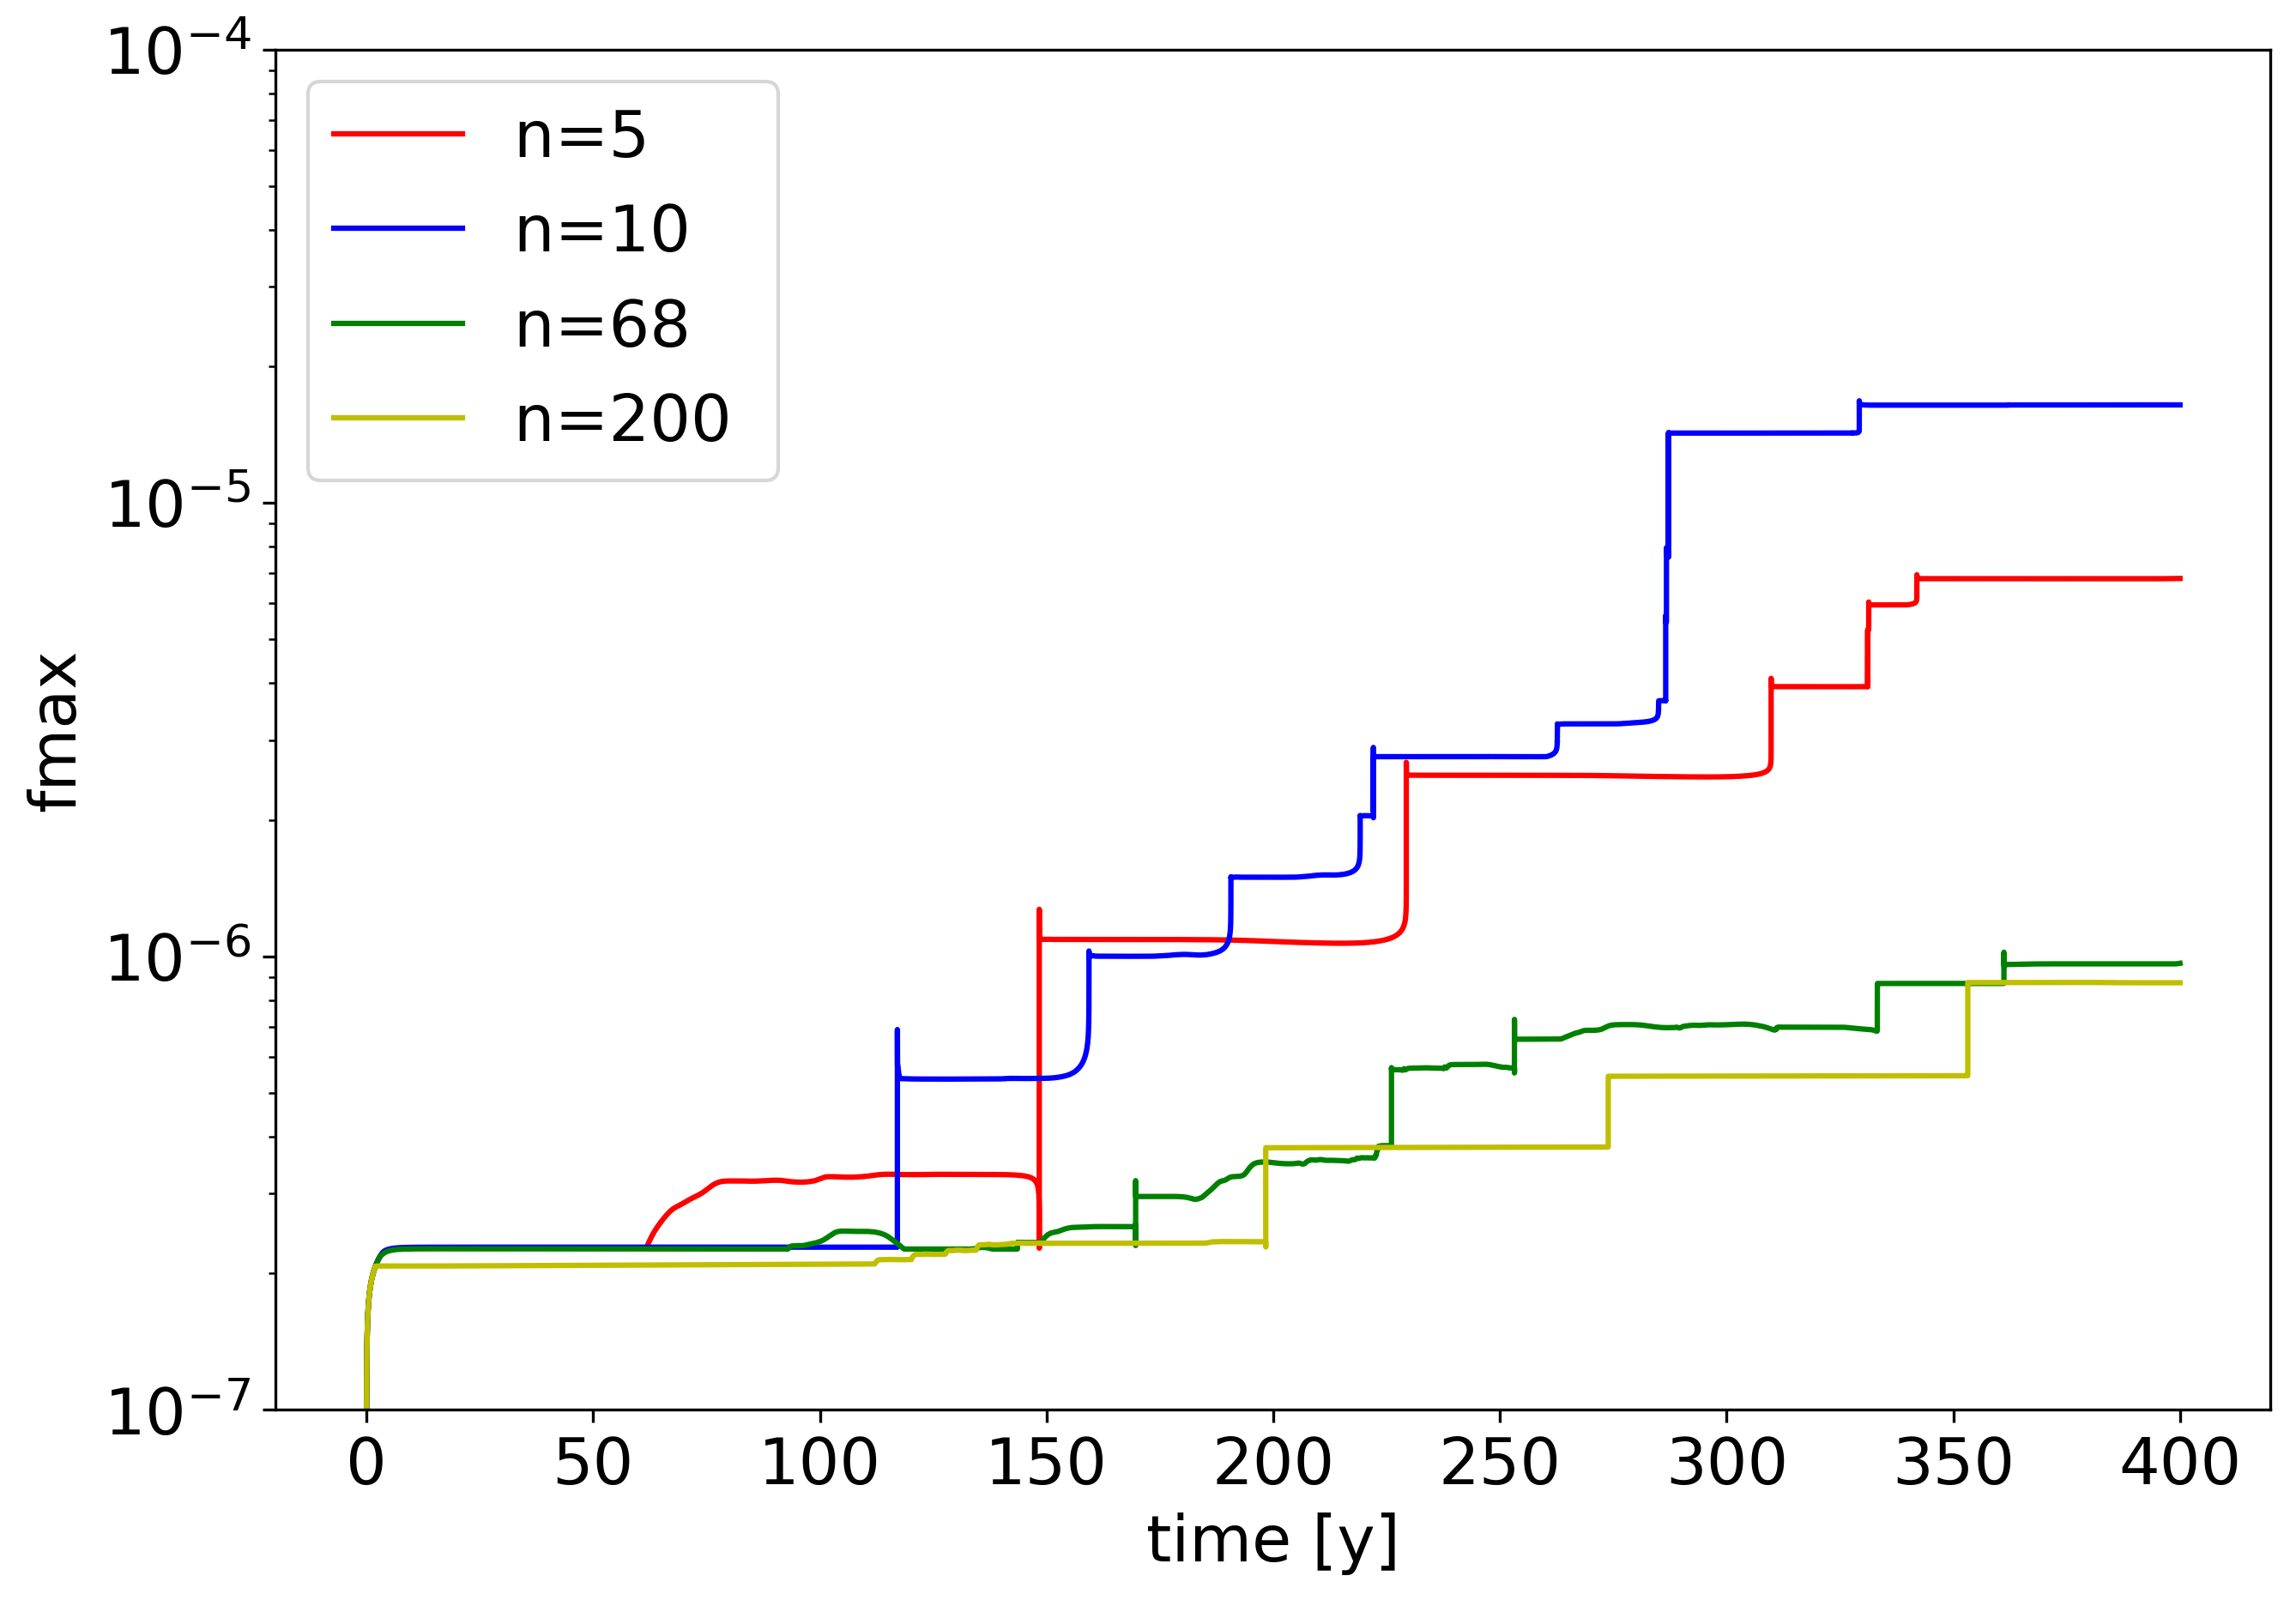
\includegraphics[width=1\textwidth]{images/TANDEMtimeEvolutionFExtendedODEDifferentSizes.png}
		\subcaption{Maximum absolute value of the friction law} 
		\label{fig:timeEvolution_2ndOrderODE_differentSizes}
	\end{subfigure}
	\begin{subfigure}{0.45\textwidth}
		\centering
		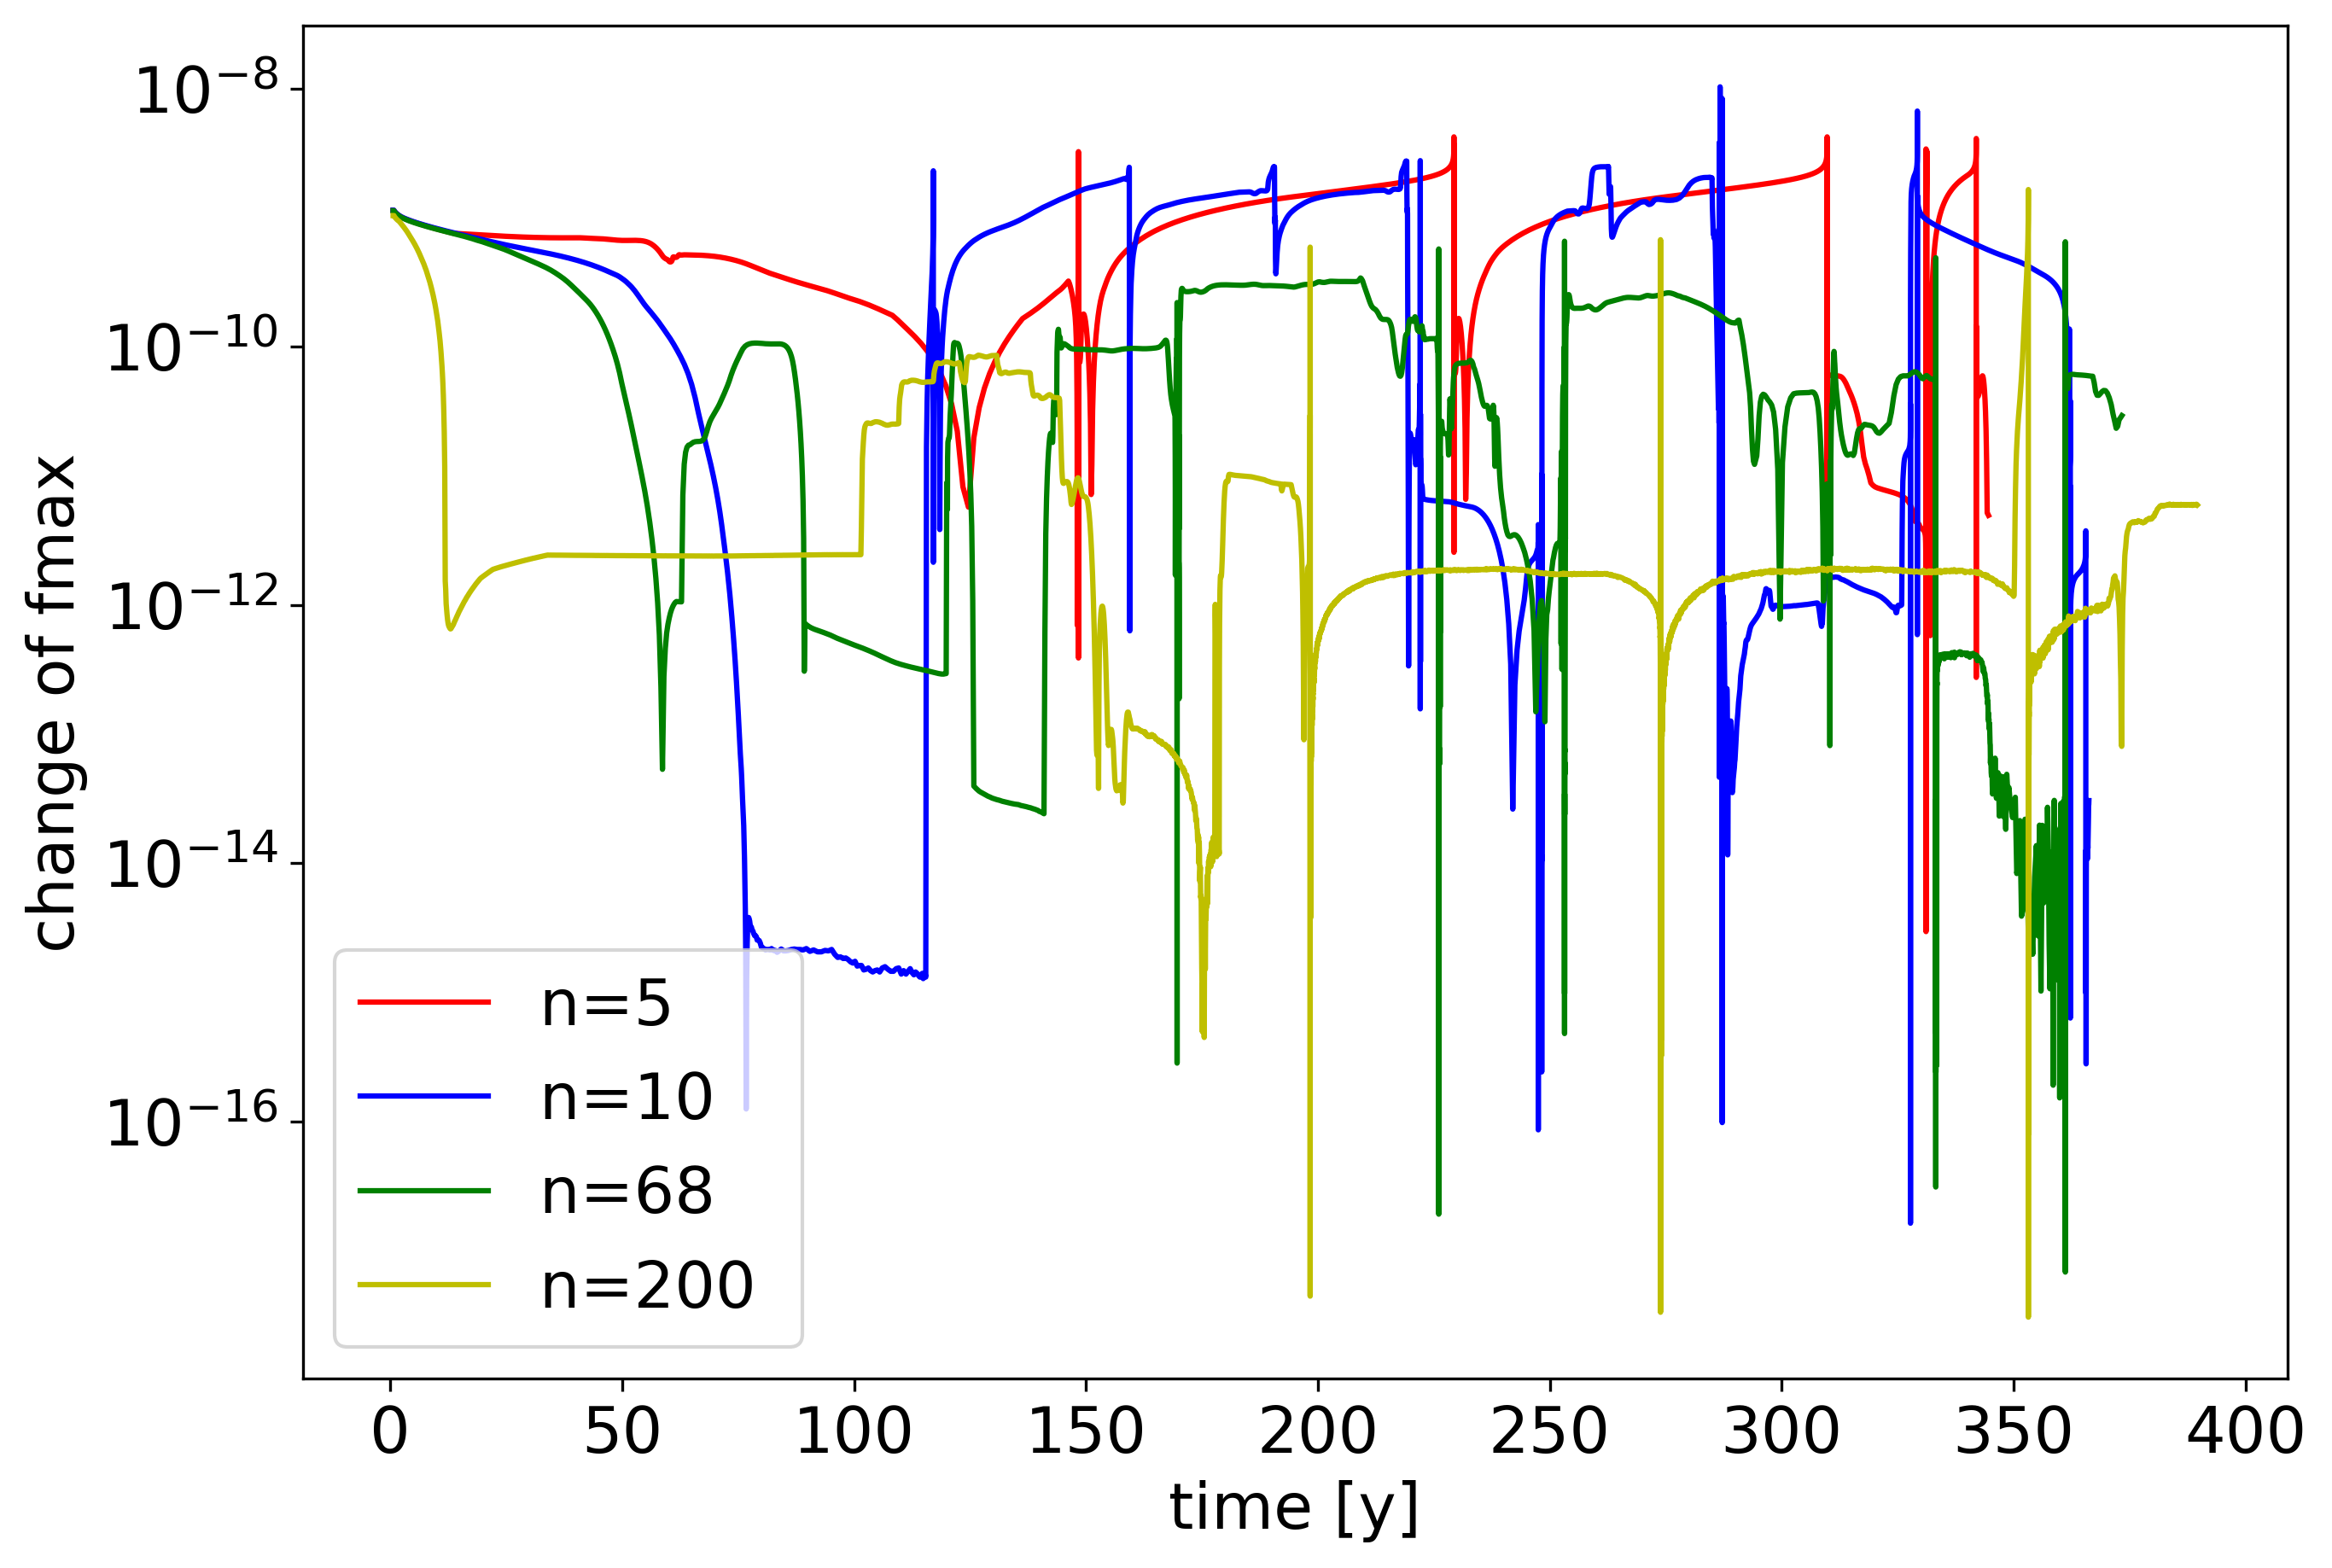
\includegraphics[width=1\textwidth]{images/TANDEMtimeEvolutionFLTEExtendedODEDifferentSizes.png}
		\subcaption{Absolute change of the friciton law per timestep, averaged over 50 timesteps} 
		\label{fig:timeEvolution_LTE_2ndOrderODE_differentSizes}
	\end{subfigure}
	\caption{Evolution of the value of the friction law of the 2nd order formulation over 400 years with varying domain sizes, where $n$ denotes the number of fault elements}
\end{figure}

Overall, the evaluation of the friction law is a suitable estimate for the global error in the system. Over the course of time, its value increases step wise at each earthquake, but overall linearly, which is due to a regular local truncation error. The main driver of the LTE is the tolerance for the slip rate $V$, which has been introduced to the system along with the second order ODE formulation. The upper bound for the LTE is proportional to the chosen tolerance.


\subsection{Analytic derivation of an upper bound for the LTE}
In this section, we try to mathematically derive an upper bound for the local truncation error from the defined tolerances in $S$, $\psi$ and $V$. With it, we can roughly estimate the error in the friction law without having to solve the Poisson problem at every timestep. 

\subsection{Normalization of the slip rate}
Does it make to evaluate the slip rate from the friction law sometimes to normalize the friction law back to if the error is to high? 

\section{Numerical treatment in SEAS}
For SEAS, the solution vector $u$ combines the velocity $V$ and the state variable $\psi$ for all interpolation points at the edge of the fault elements. The functional $F$ is not used and takes as value only the time derivative of the solution vector $\dot{u}$. The call of the right-hand-side function $G(u,t)$ combines the solving of the algebraic and the differential equations. At each step, following steps are performed: 
\begin{enumerate}
    \item The current displacement in the whole system is calculated to fulfill the Poisson or elasticity equations by solving \autoref{eq:SEAS_DAE_AU=b} \\
    \item The values of $\tau(U)$ and $\sigma_n(U)$ are calculated on the fault according to the updated displacements \\
    \item The iteration over all interpolation points on the fault is performed. At each interpolation step: 
    \begin{itemize}
        \item the velocity $V_i$ is obtained from the friction law in \autoref{eq:SEASDAE_frictionLaw} with the bisection method,
        \item and the actual right hand side $G(u,t)$ of the ODE is evaluated using equations \ref{eq:SEAS_DAE_ageing_law} and \ref{eq:SEASDAE_dV_dt}.
    \end{itemize}
\end{enumerate}


\subsection{Explicit methods}
Runge-Kutta schemes with error correction term 
\begin{itemize}
    \item Bogacki-Shampine (RKBS3): 2nd order with 3rd order error correction \\
    \item Dormand-Prince (RKDP5): 4th order with 5th order error correction 
\end{itemize}

\subsection{Implicit methods}
BDF methods of order 1-6
describe coefficients and error estimation with Lagrange polynomials
t method
\subsection{Implicit - explicit methods}
Not really a thing yet, but consider for later. Needs to reformulate the DAE with a nonzero G(), can only be used for the ageing law g().

\subsection{Switching between different formulations}
 --> next thing to implement
 
\subsection{Definition of the tolerances}


\subsection{Time adaptivity}

\section{Results}
\subsection{Comparison between the different formulations of problem}
The simulation is run over a period of 250 years, in which one earthquake occurs on June 13th of the 195th year. This event can be clearly observed in \autoref{fig:timeEvolutionTANDEM_V} which depicts the maximum slip rate over time, which reaches $4.6m\cdot s^{-1}$ as opposed to an average of $1.0 \cdot 10^{-9}m\cdot s^{-1}$ in calm times. 
\begin{figure}[H]
    \centering
    \begin{subfigure}{0.32\textwidth}
     	\centering
    	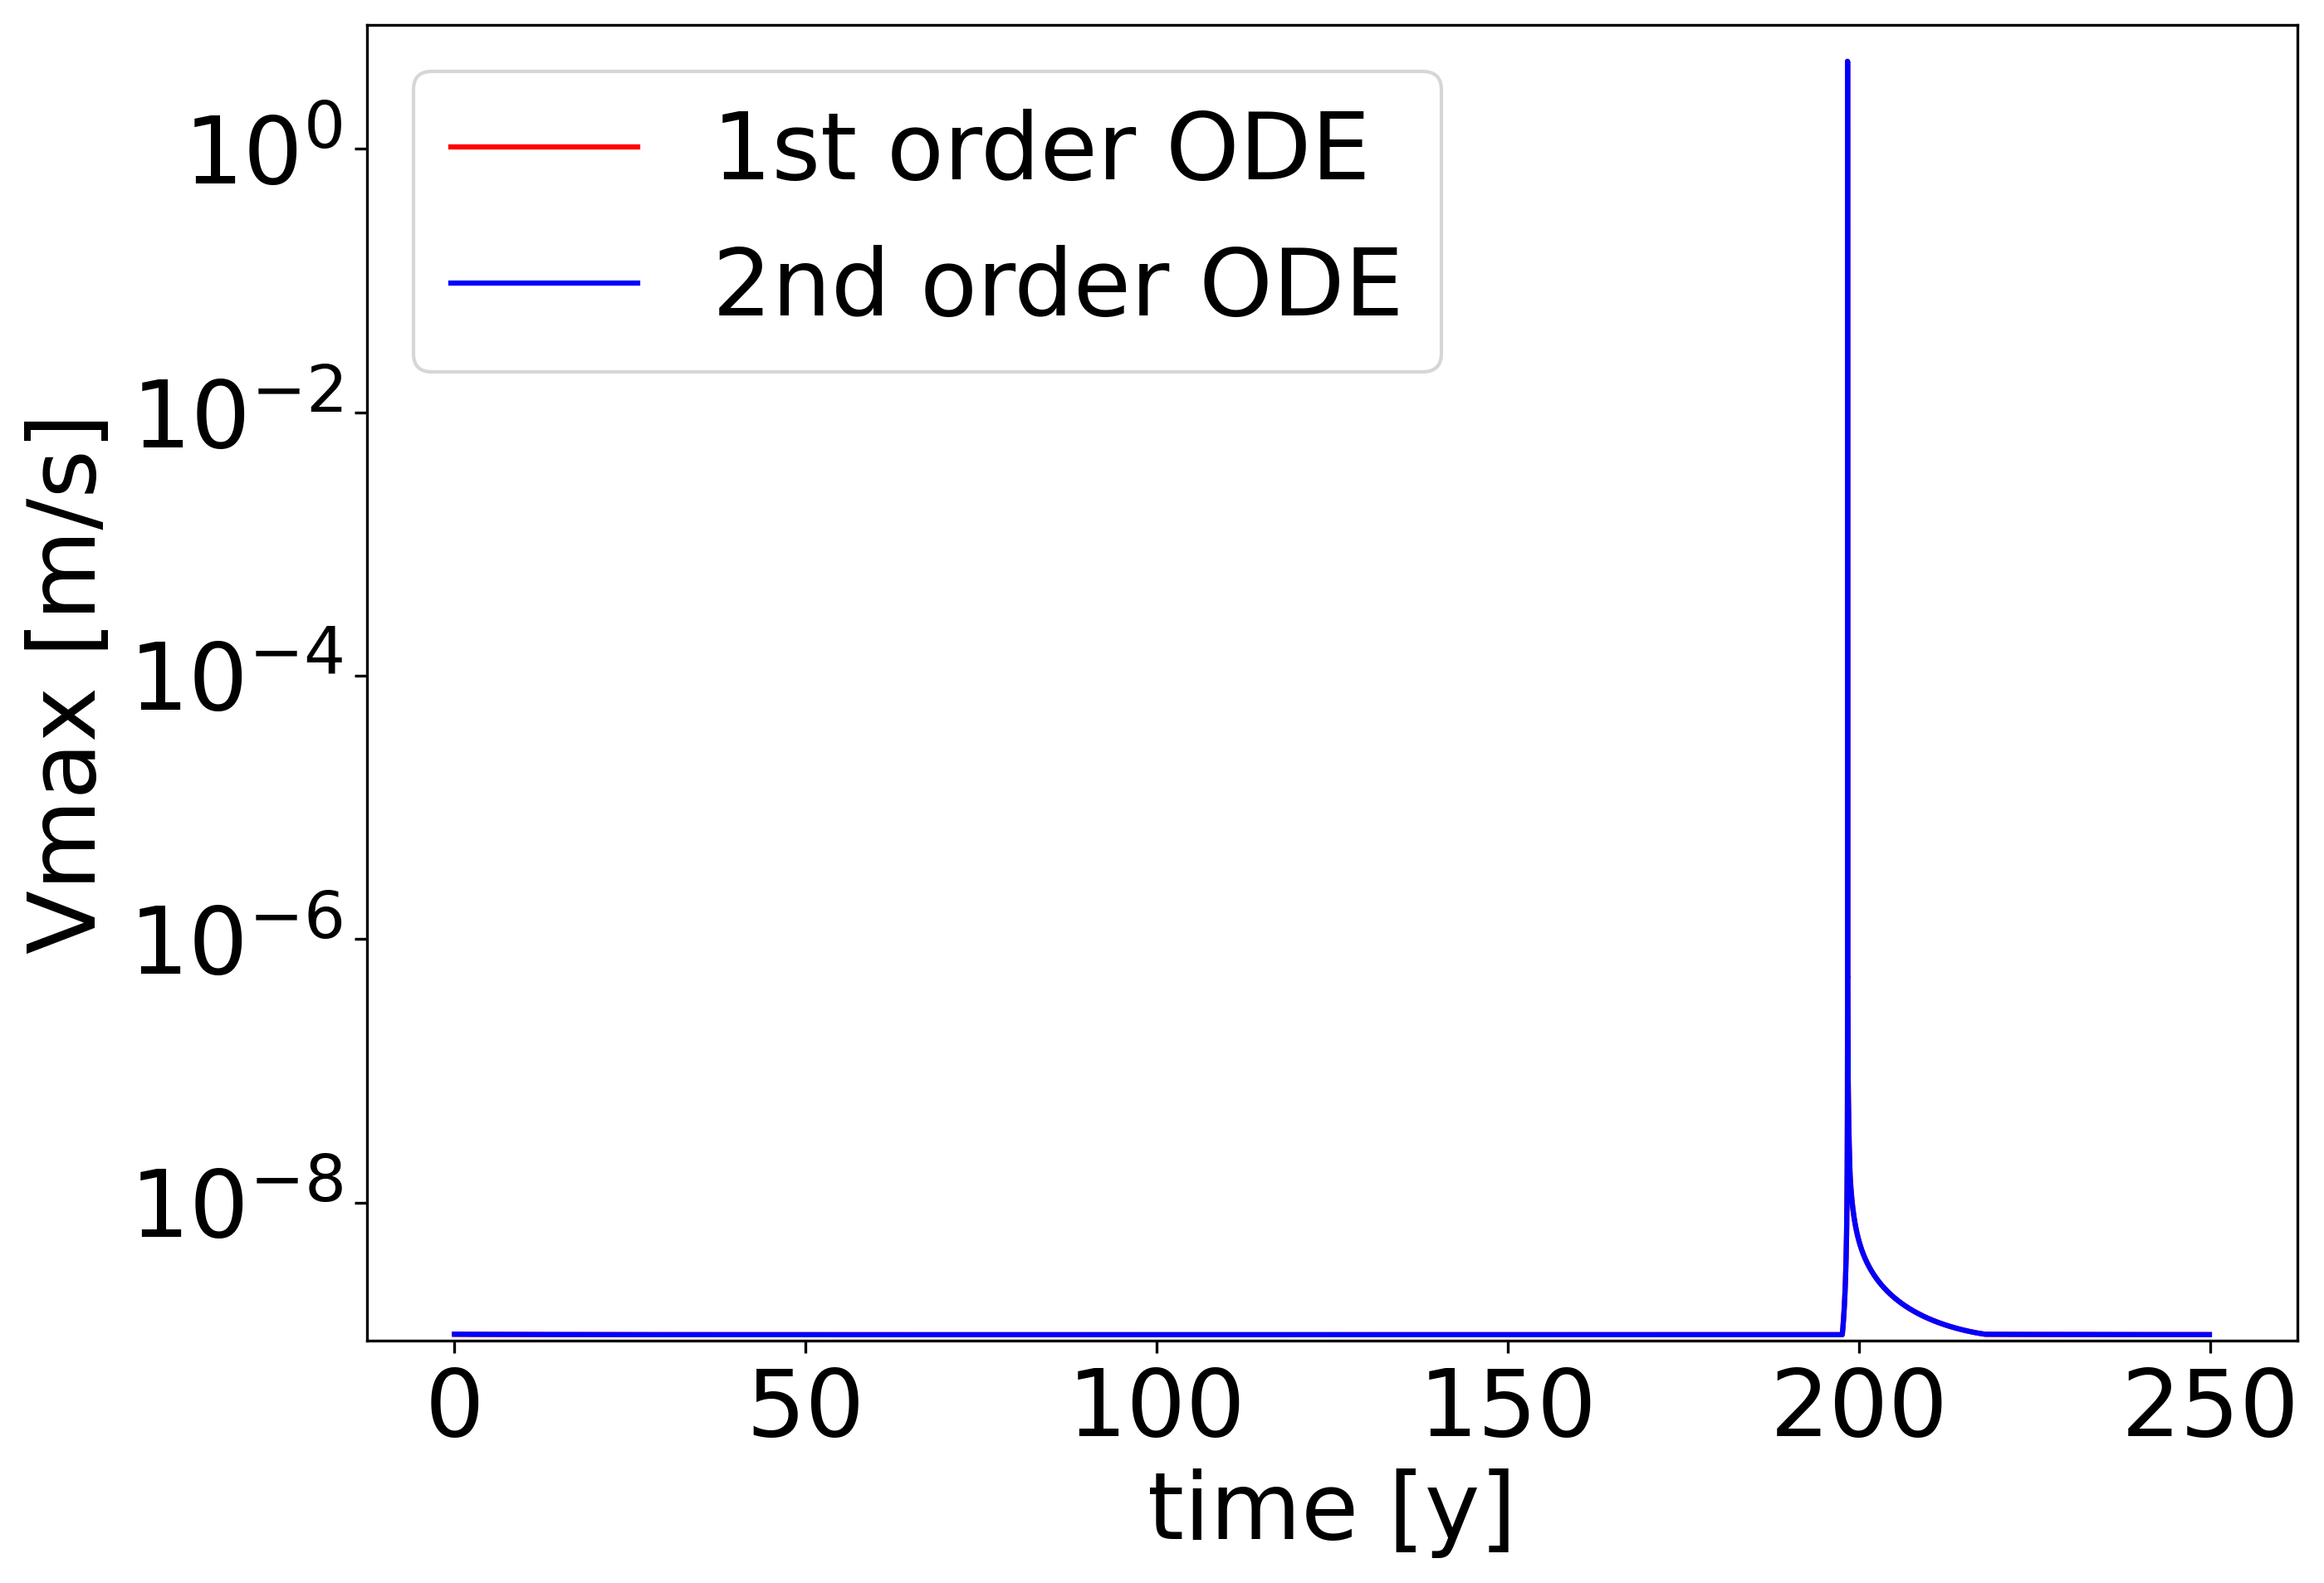
\includegraphics[width=1\textwidth]{images/TANDEMcompareFormulationstimeEvolutionVall.png}
       	\subcaption{Full simulation time} 
    \end{subfigure} 
    \begin{subfigure}{0.32\textwidth}
    	\centering
    	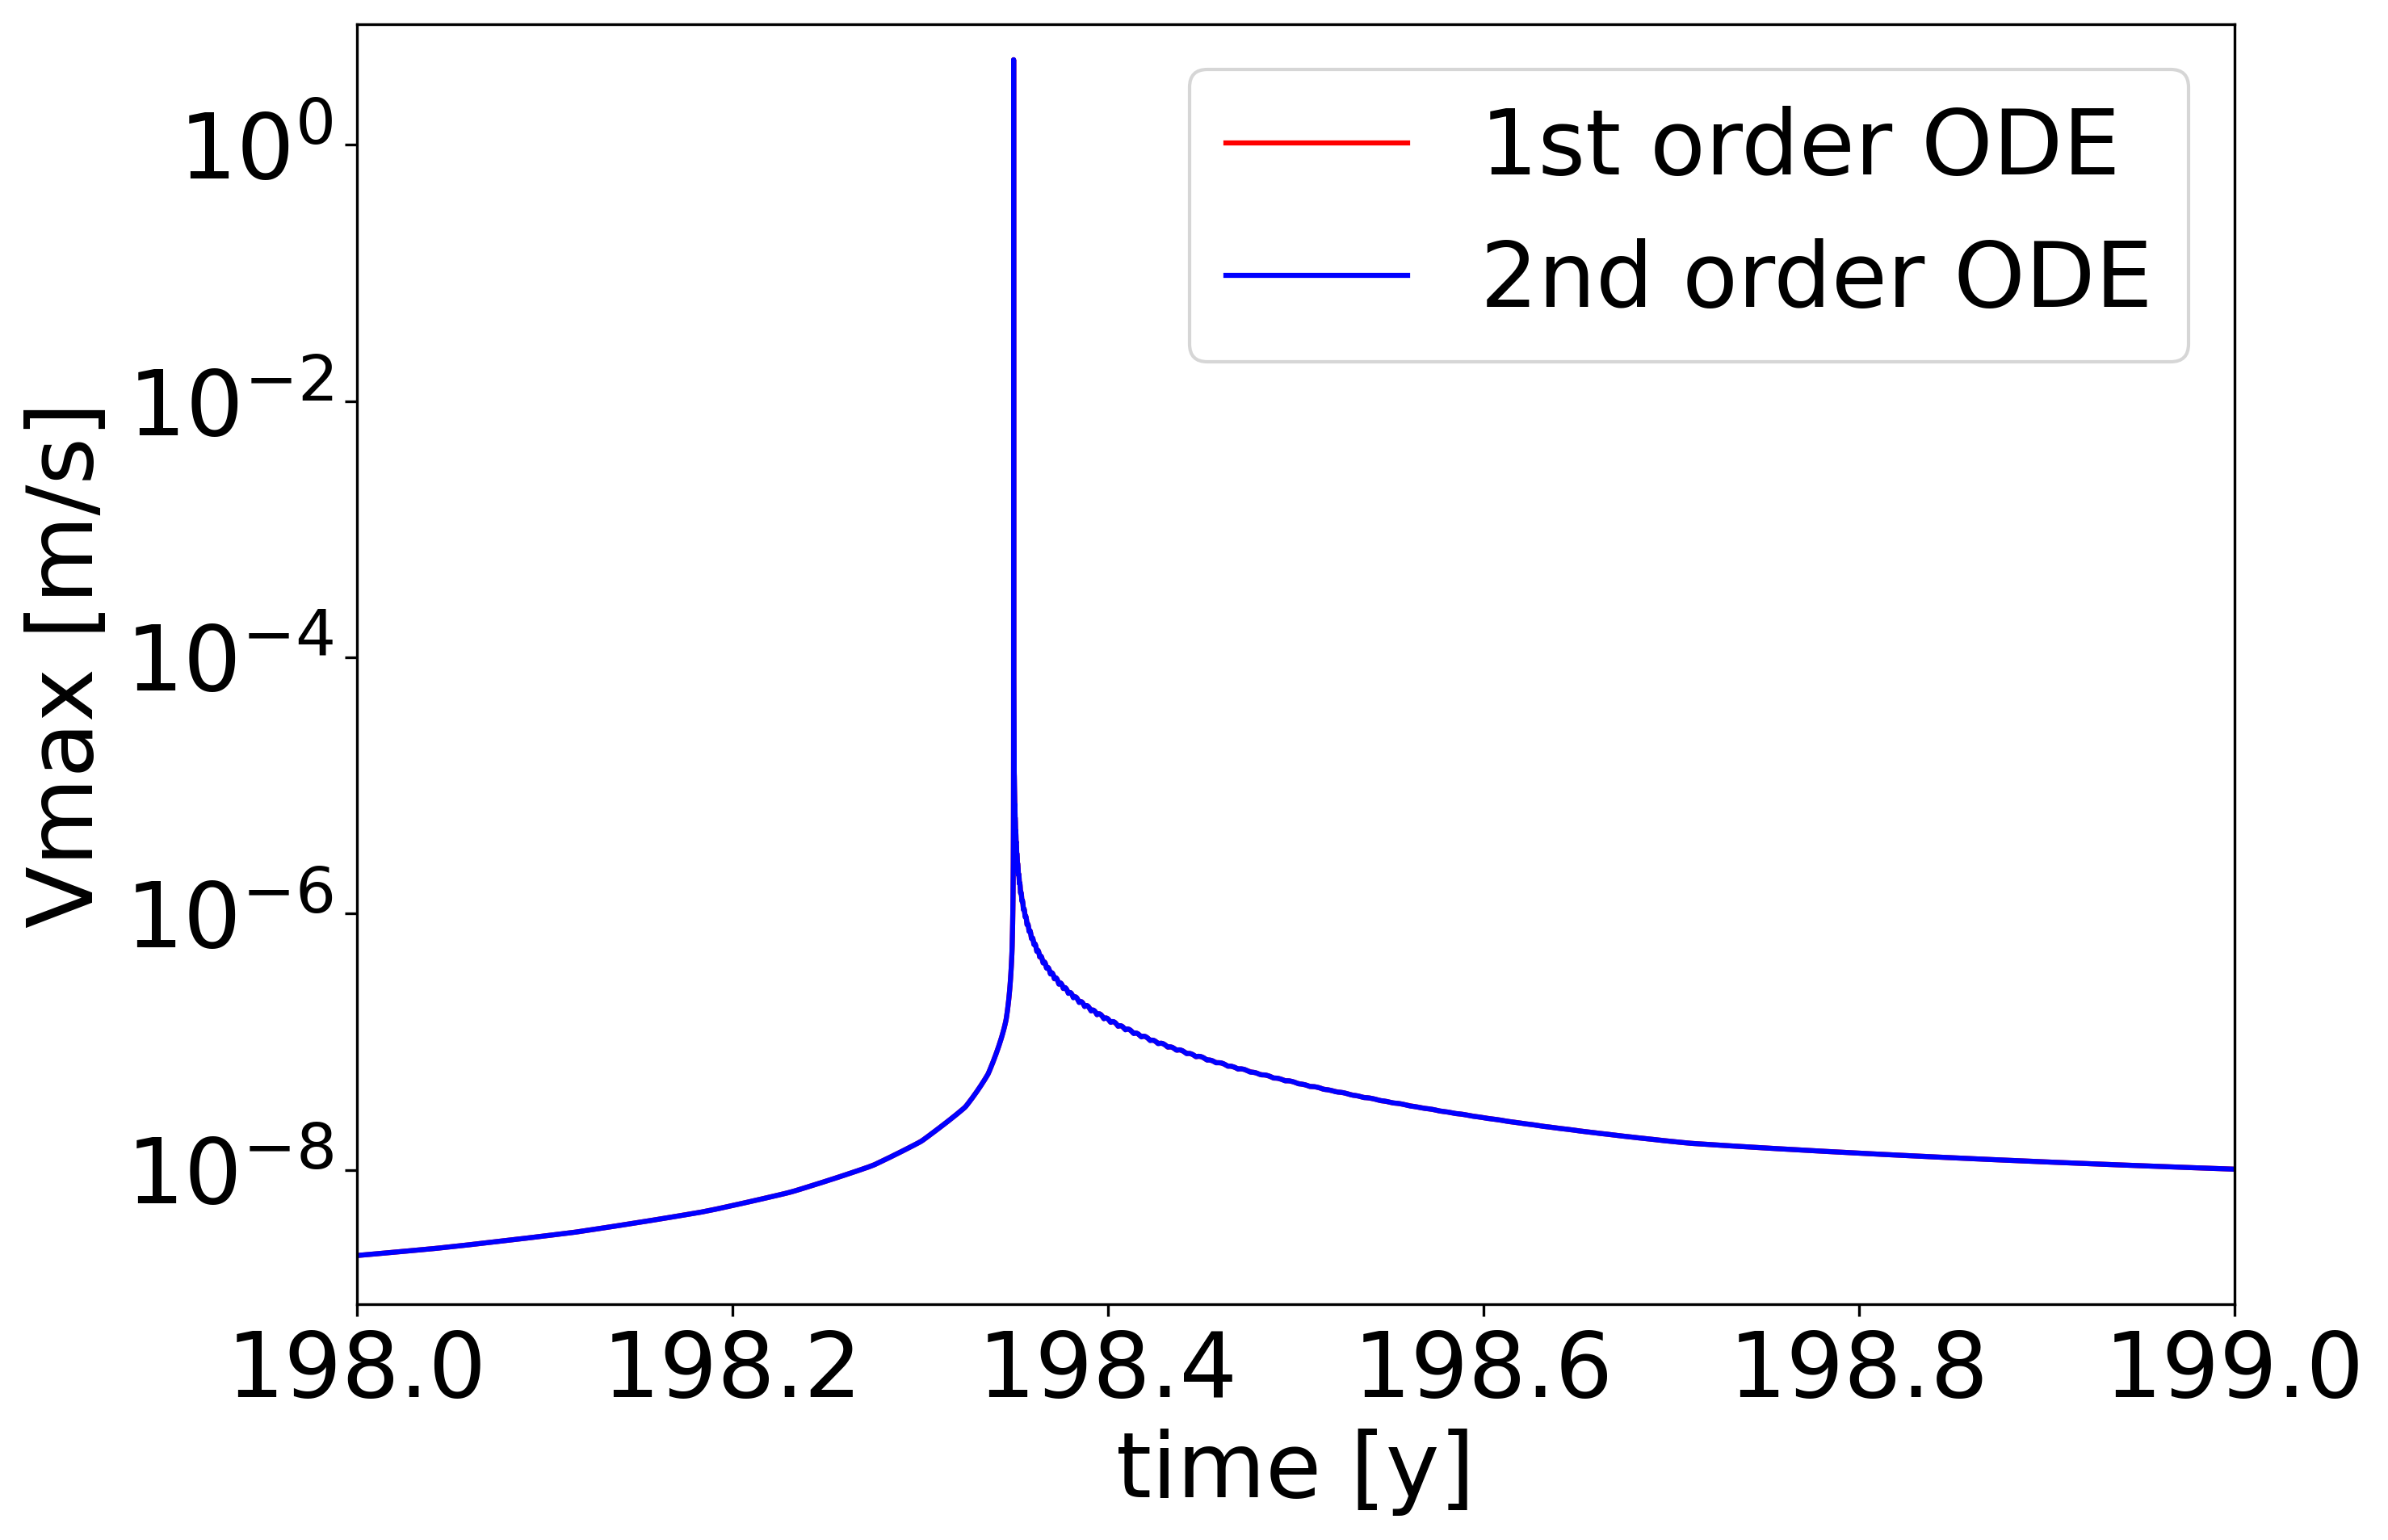
\includegraphics[width=1\textwidth]{images/TANDEMcompareFormulationstimeEvolutionVsurroundings.png}
       	\subcaption{Year of the earthquake} 
    \end{subfigure}
    \begin{subfigure}{0.32\textwidth}
    	\centering
    	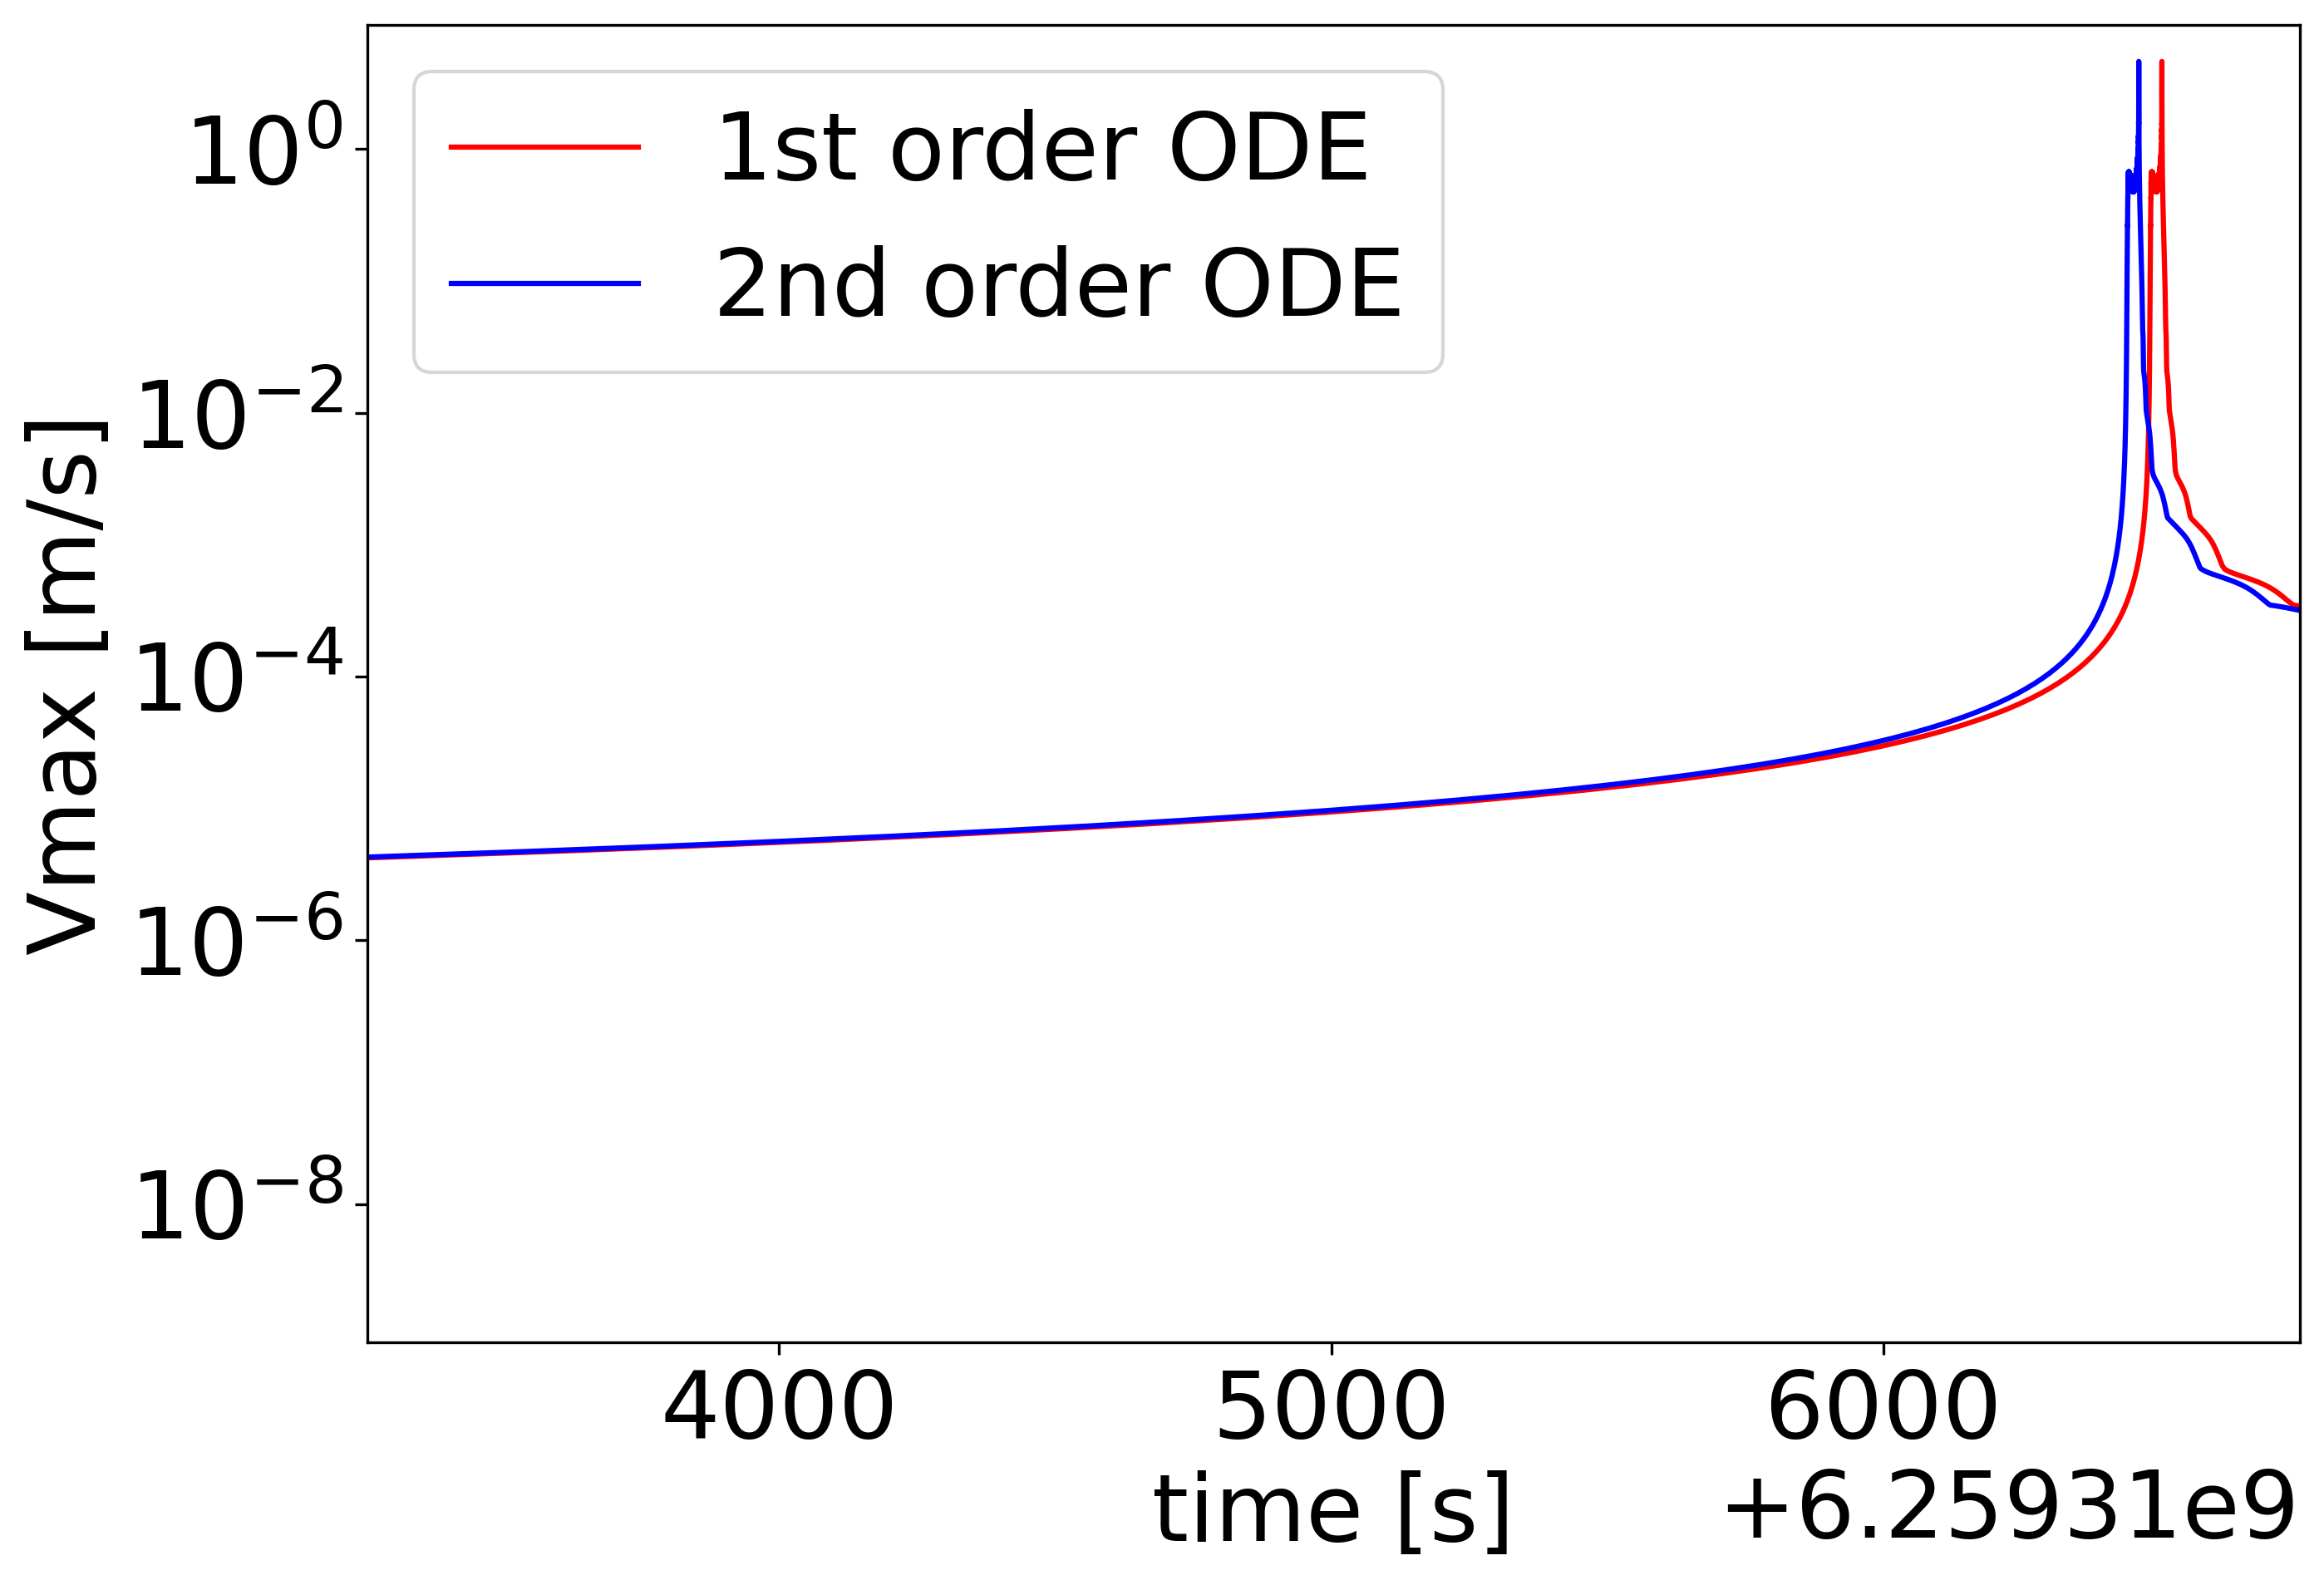
\includegraphics[width=1\textwidth]{images/TANDEMcompareFormulationstimeEvolutionVearthquake.png}
       	\subcaption{Evolution of the earthquake event} 
    \end{subfigure}
    \caption{Evolution of the maximal slip rate $V$ on the fault for different solvers on the symmetric two-dimensional BP1 problem with 200 elements on the fault}
    \label{fig:timeEvolutionTANDEM_V}
\end{figure}


\begin{figure}[H]
    \centering
    \begin{subfigure}{0.32\textwidth}
    	\centering
    	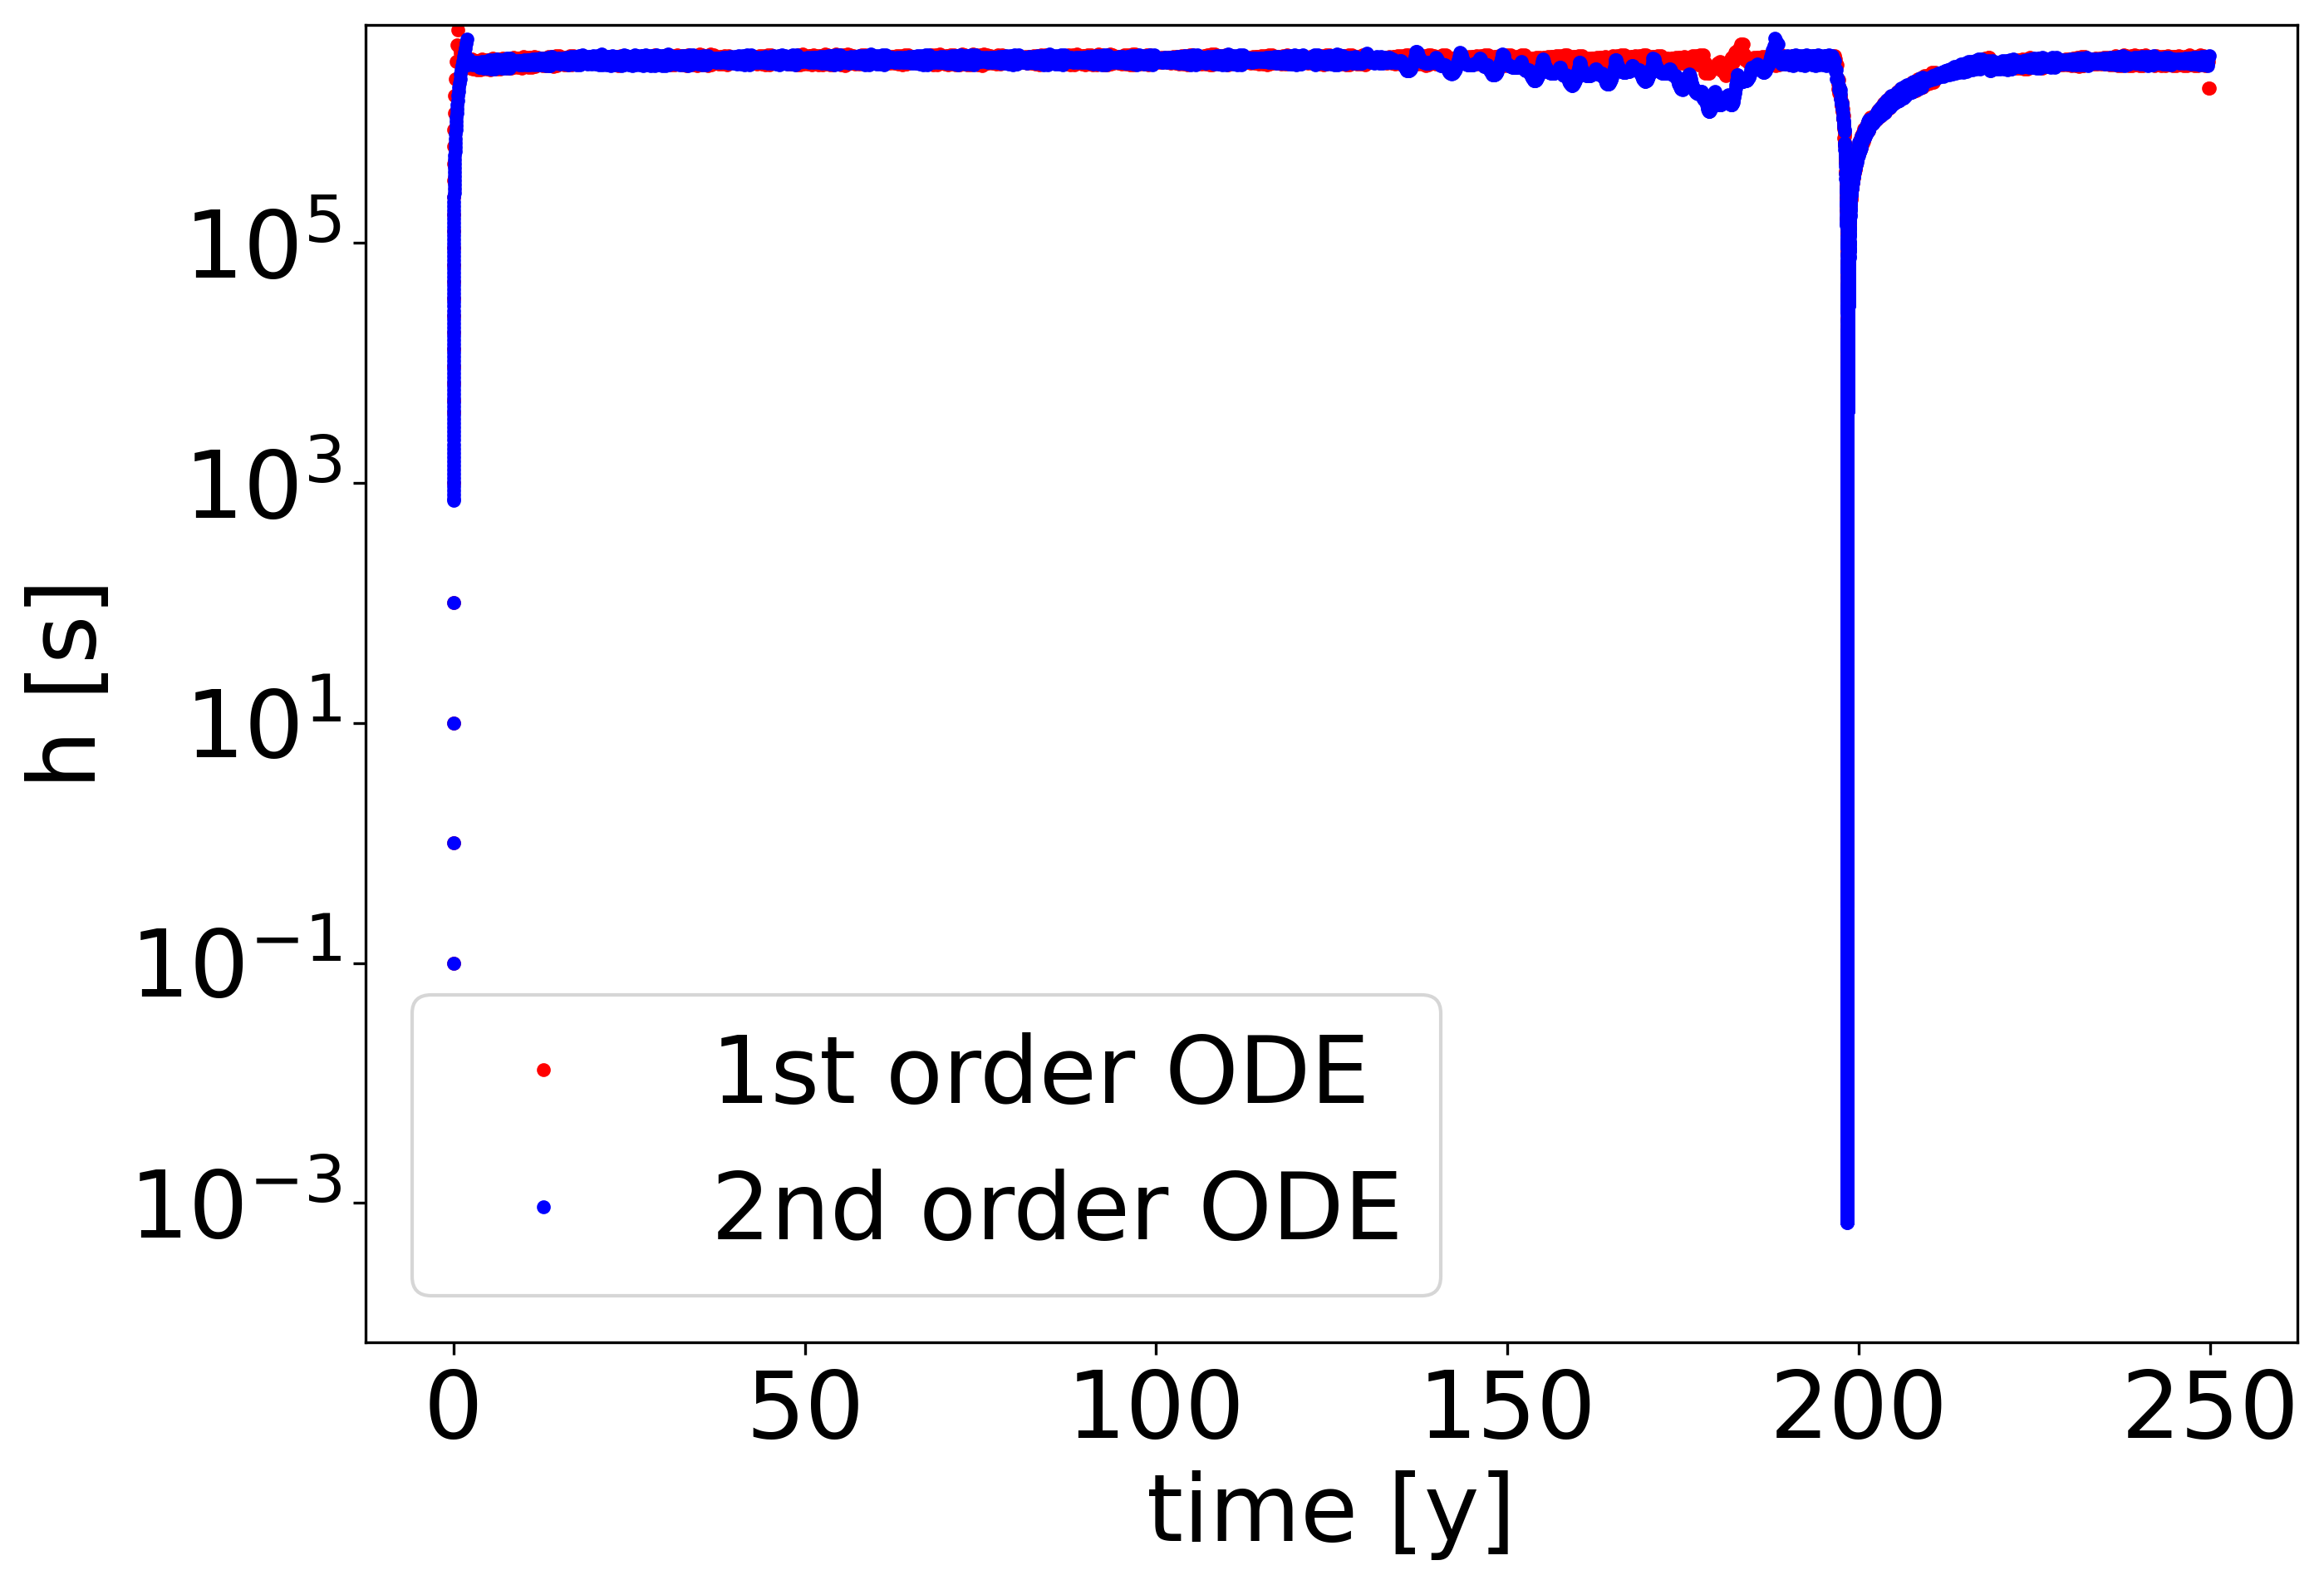
\includegraphics[width=1\textwidth]{images/TANDEMcompareFormulationstimeEvolutionDTall.png}
       	\subcaption{Full simulation time} 
    \end{subfigure}
    \begin{subfigure}{0.32\textwidth}
    	\centering
    	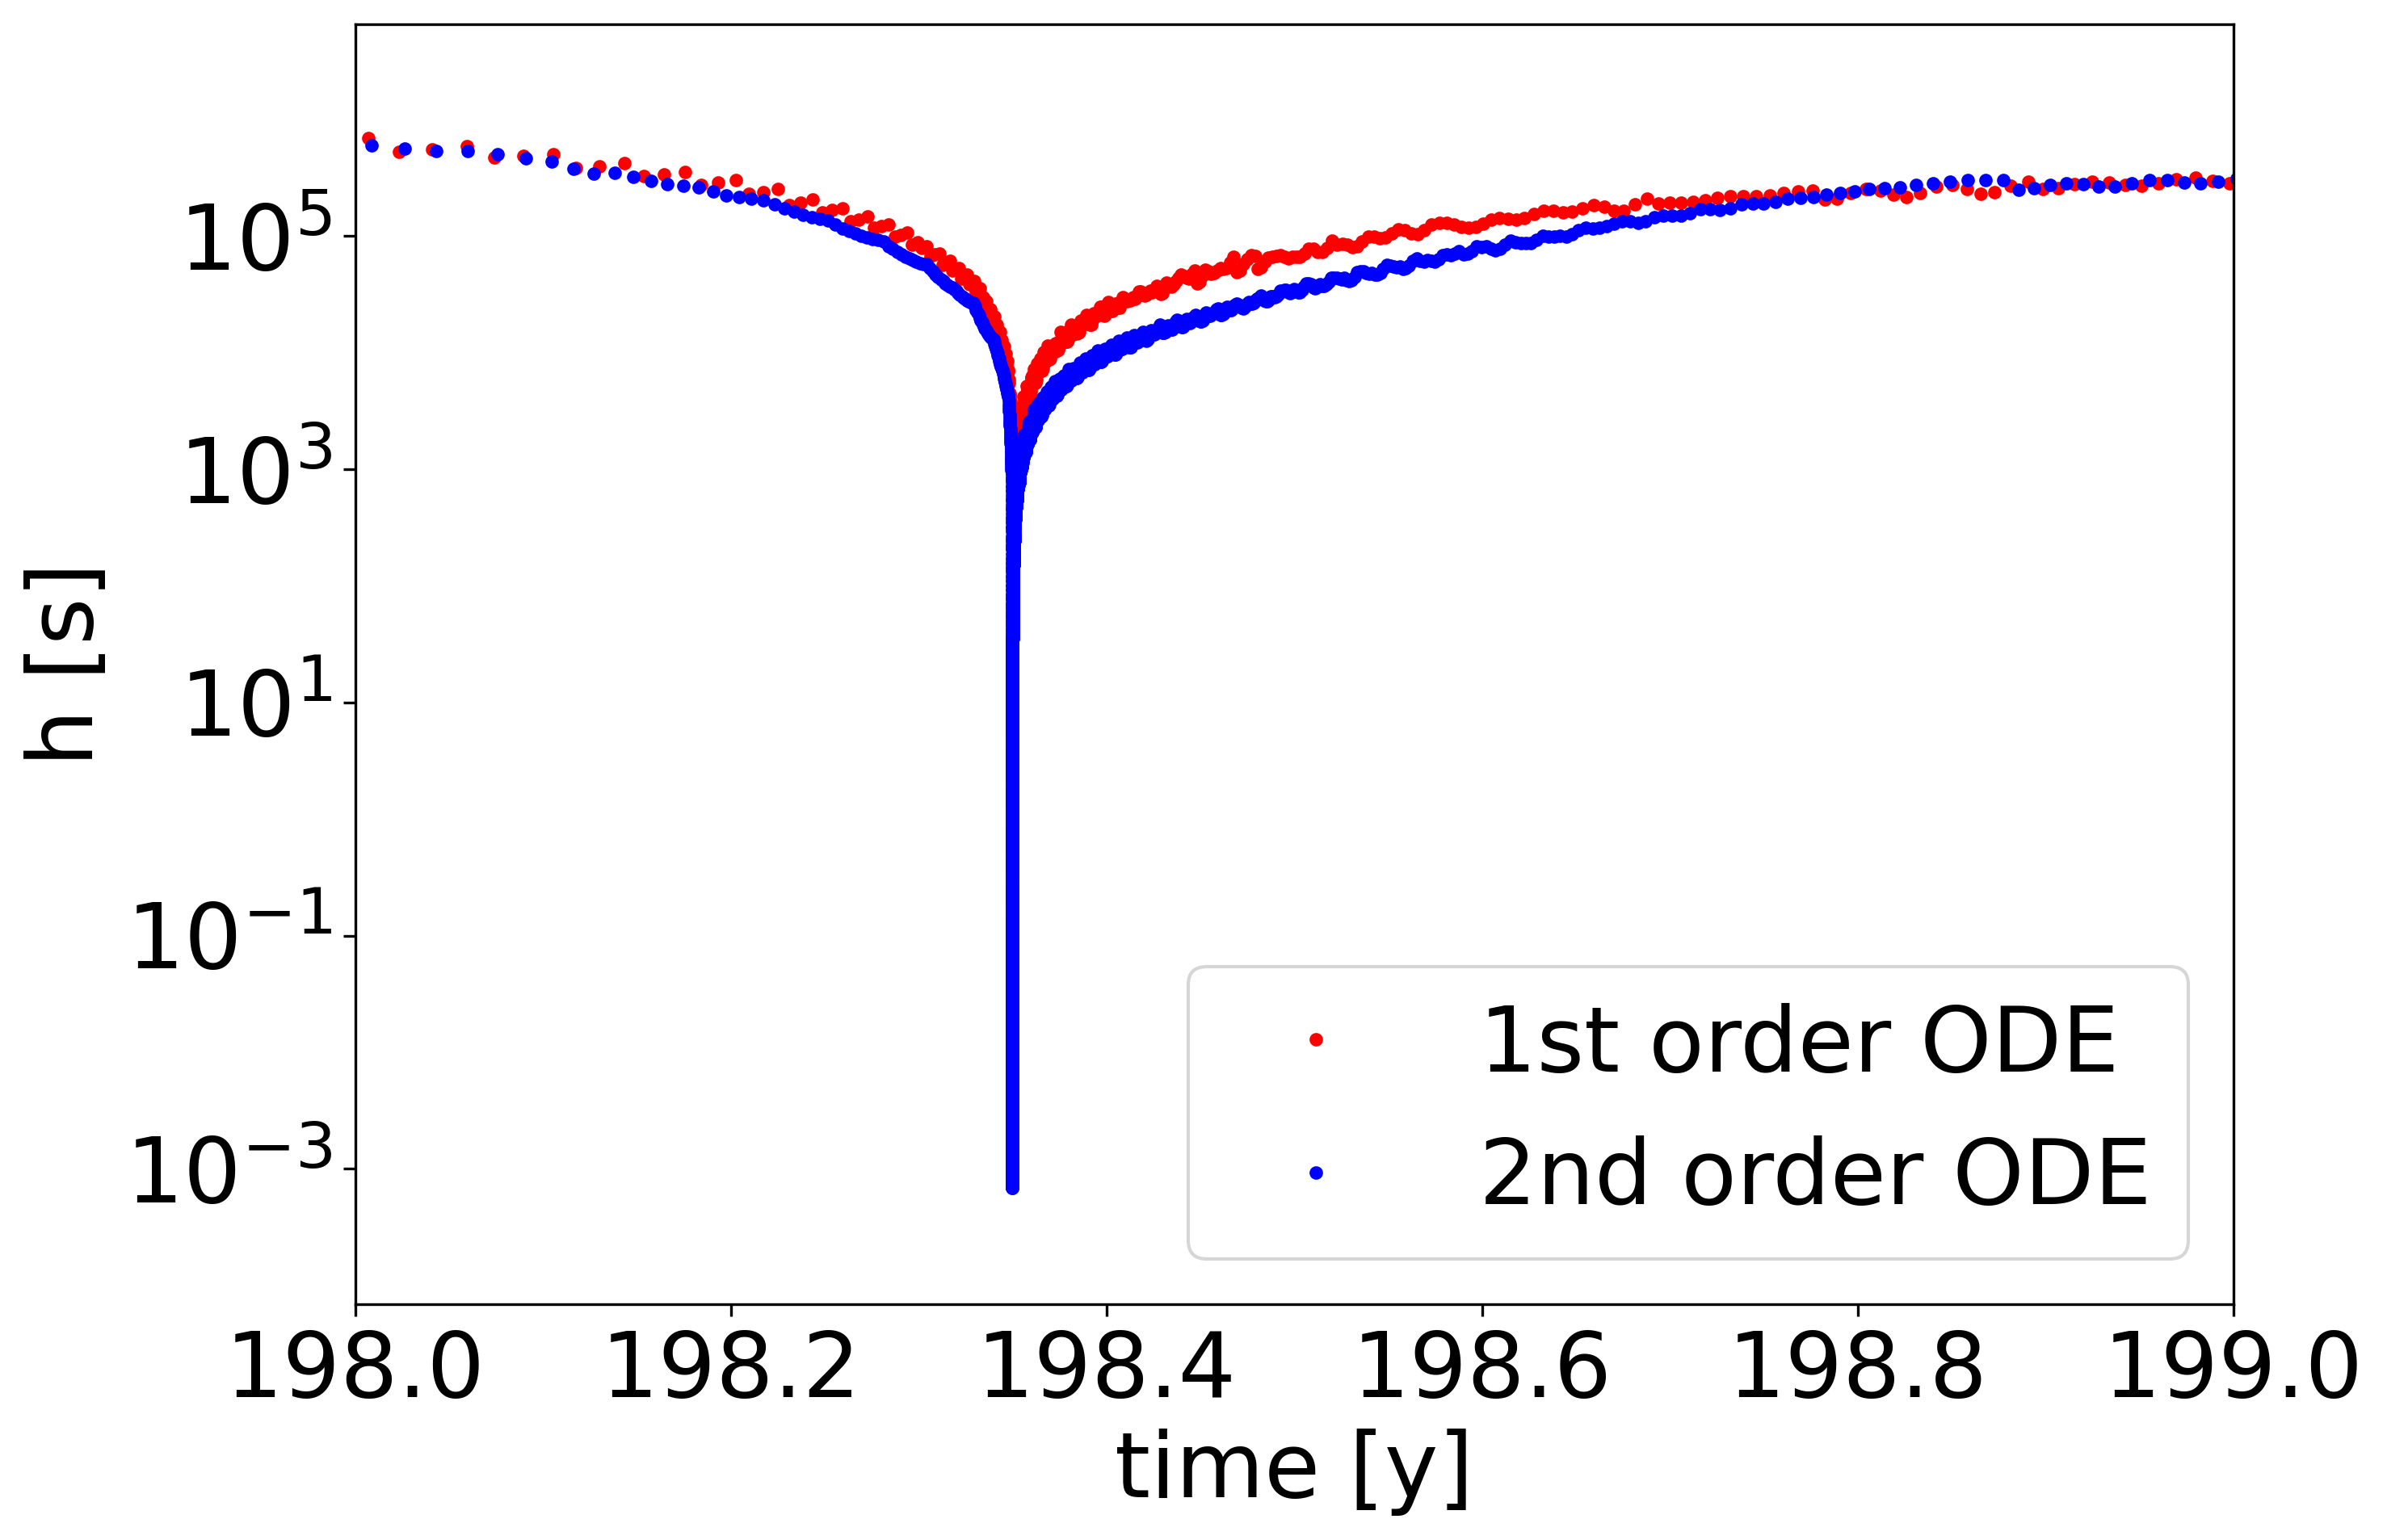
\includegraphics[width=1\textwidth]{images/TANDEMcompareFormulationstimeEvolutionDTsurroundings.png}
       	\subcaption{Year of the earthquake} 
    \end{subfigure}
    \begin{subfigure}{0.32\textwidth}
    	\centering
    	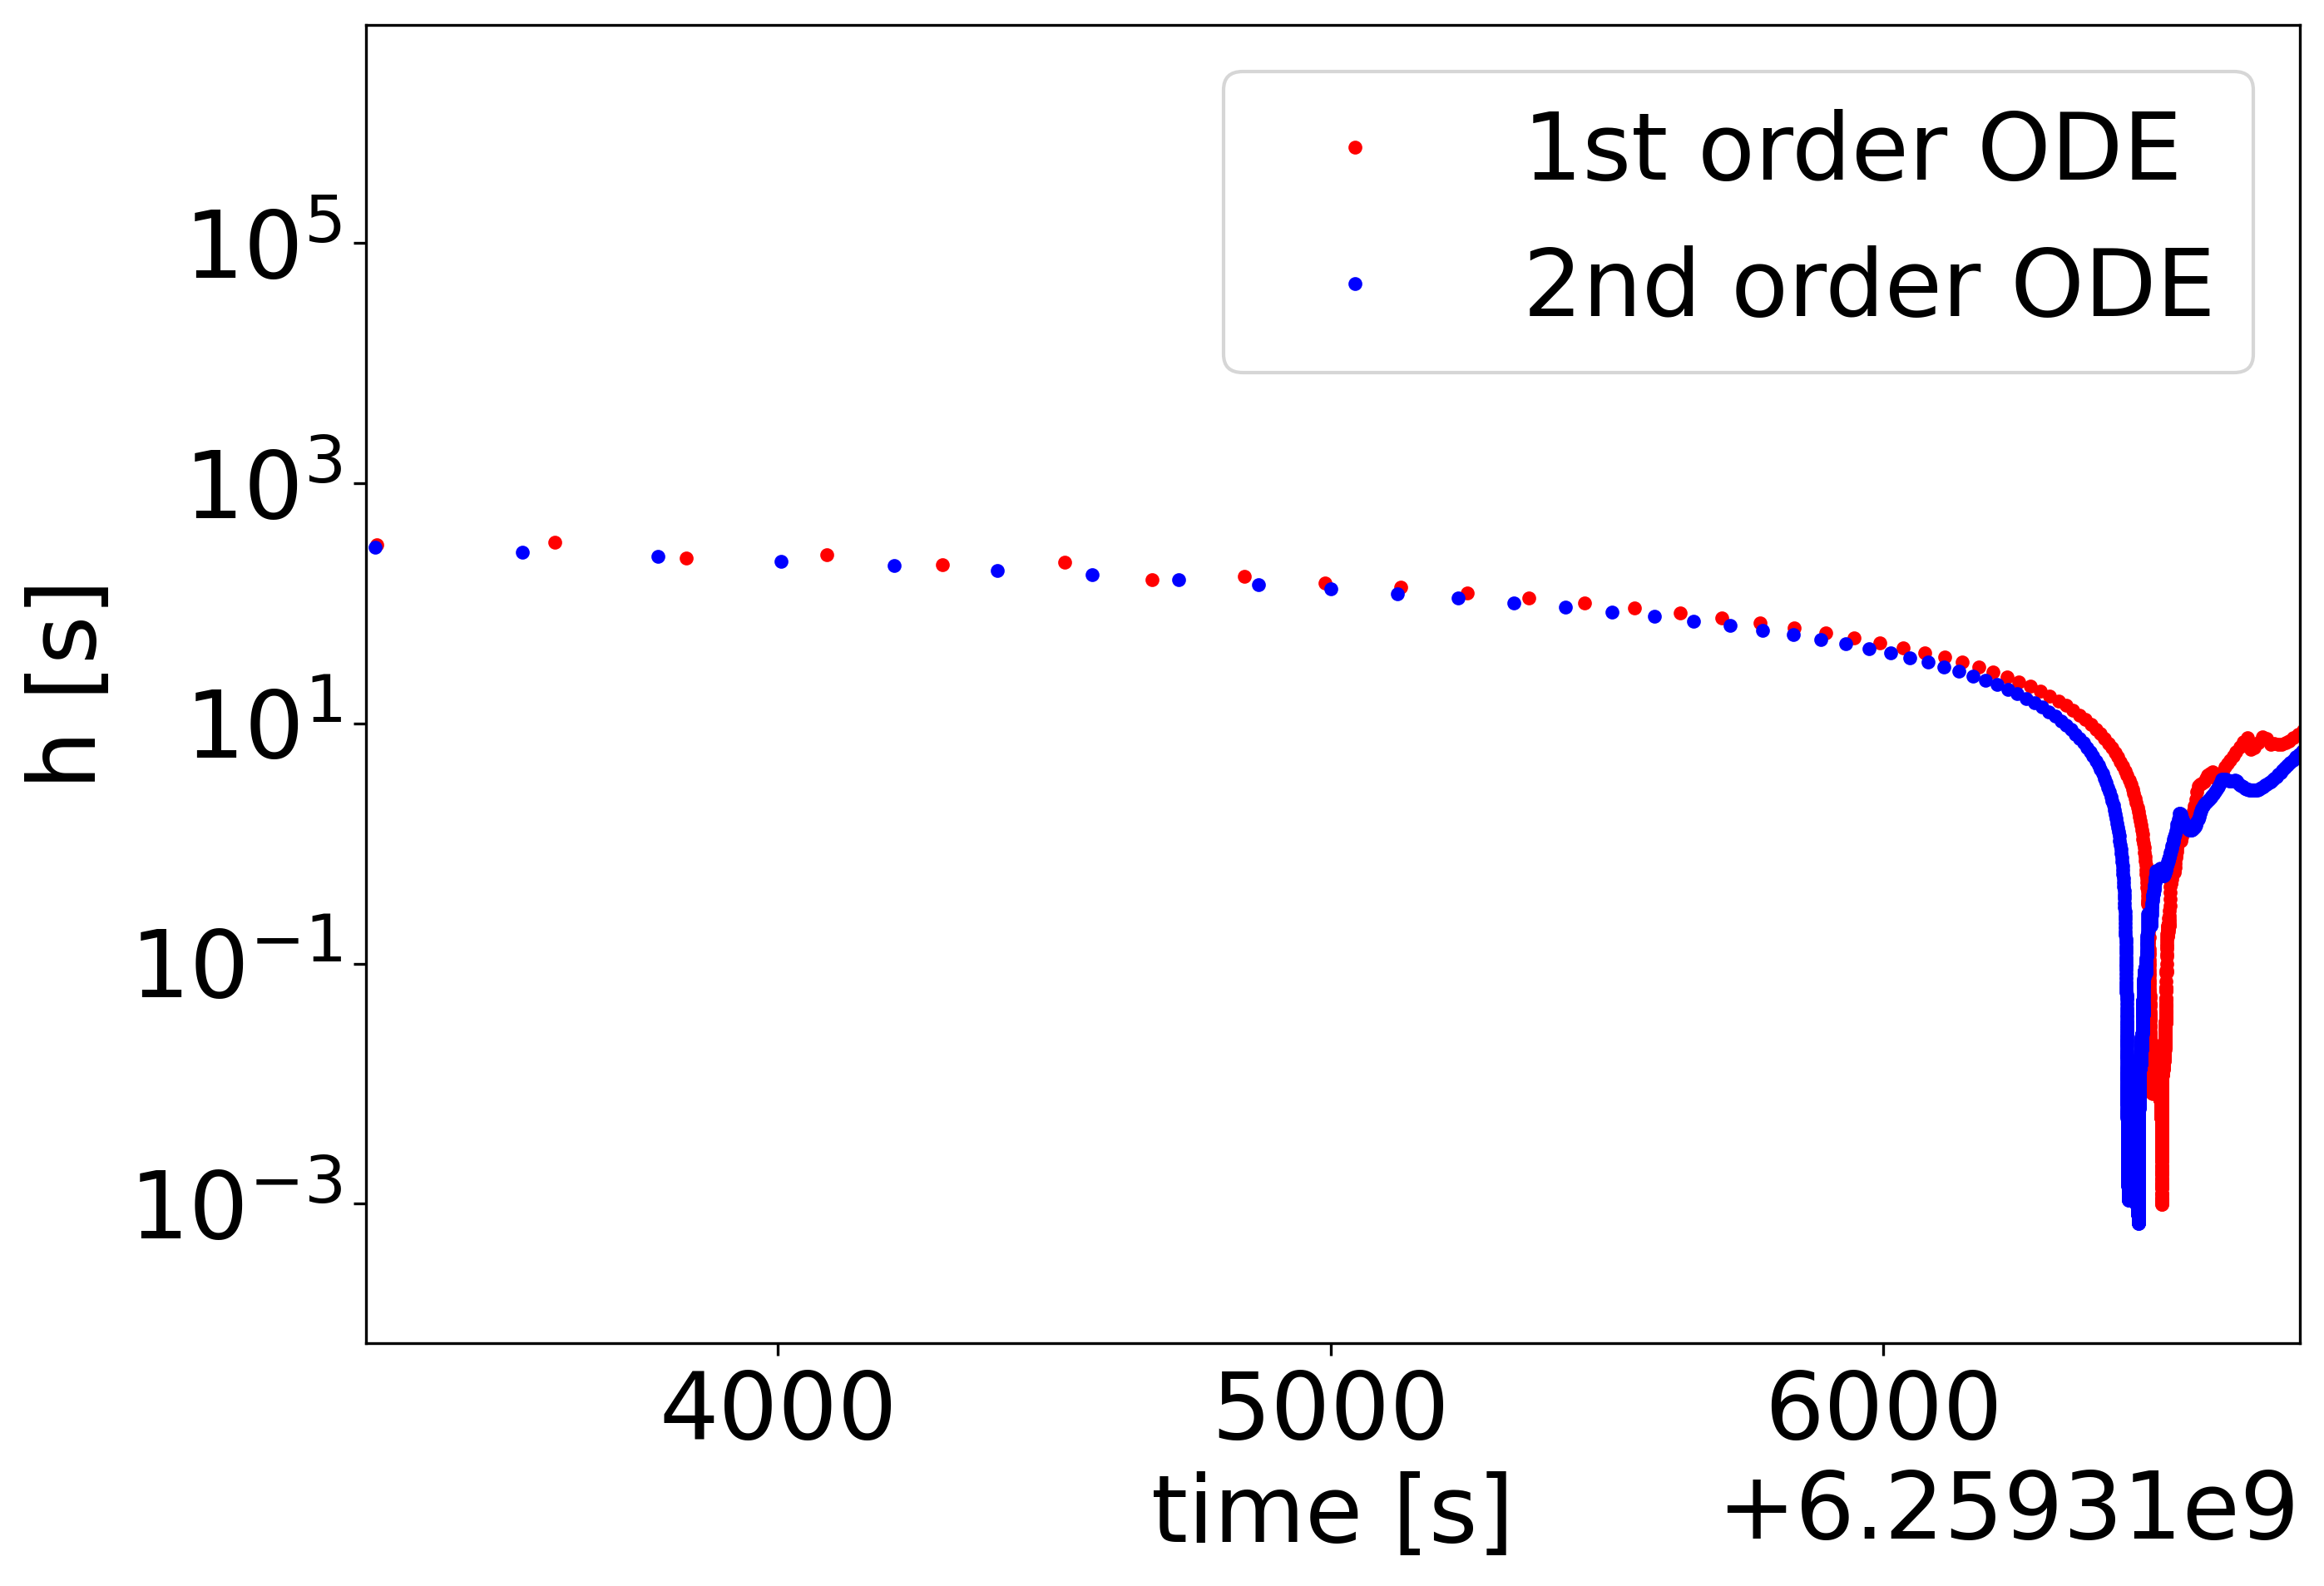
\includegraphics[width=1\textwidth]{images/TANDEMcompareFormulationstimeEvolutionDTearthquake.png}
       	\subcaption{Evolution of the earthquake event} 
    \end{subfigure}
    \caption{Evolution of the time step size $h$ for different solvers on the symmetric two-dimensional BP1 problem with 200 elements on the fault}
    \label{fig:timeEvolutionTANDEM_DT}
\end{figure}


\begin{figure}[H]
    \centering
    \begin{subfigure}{0.32\textwidth}
    	\centering
    	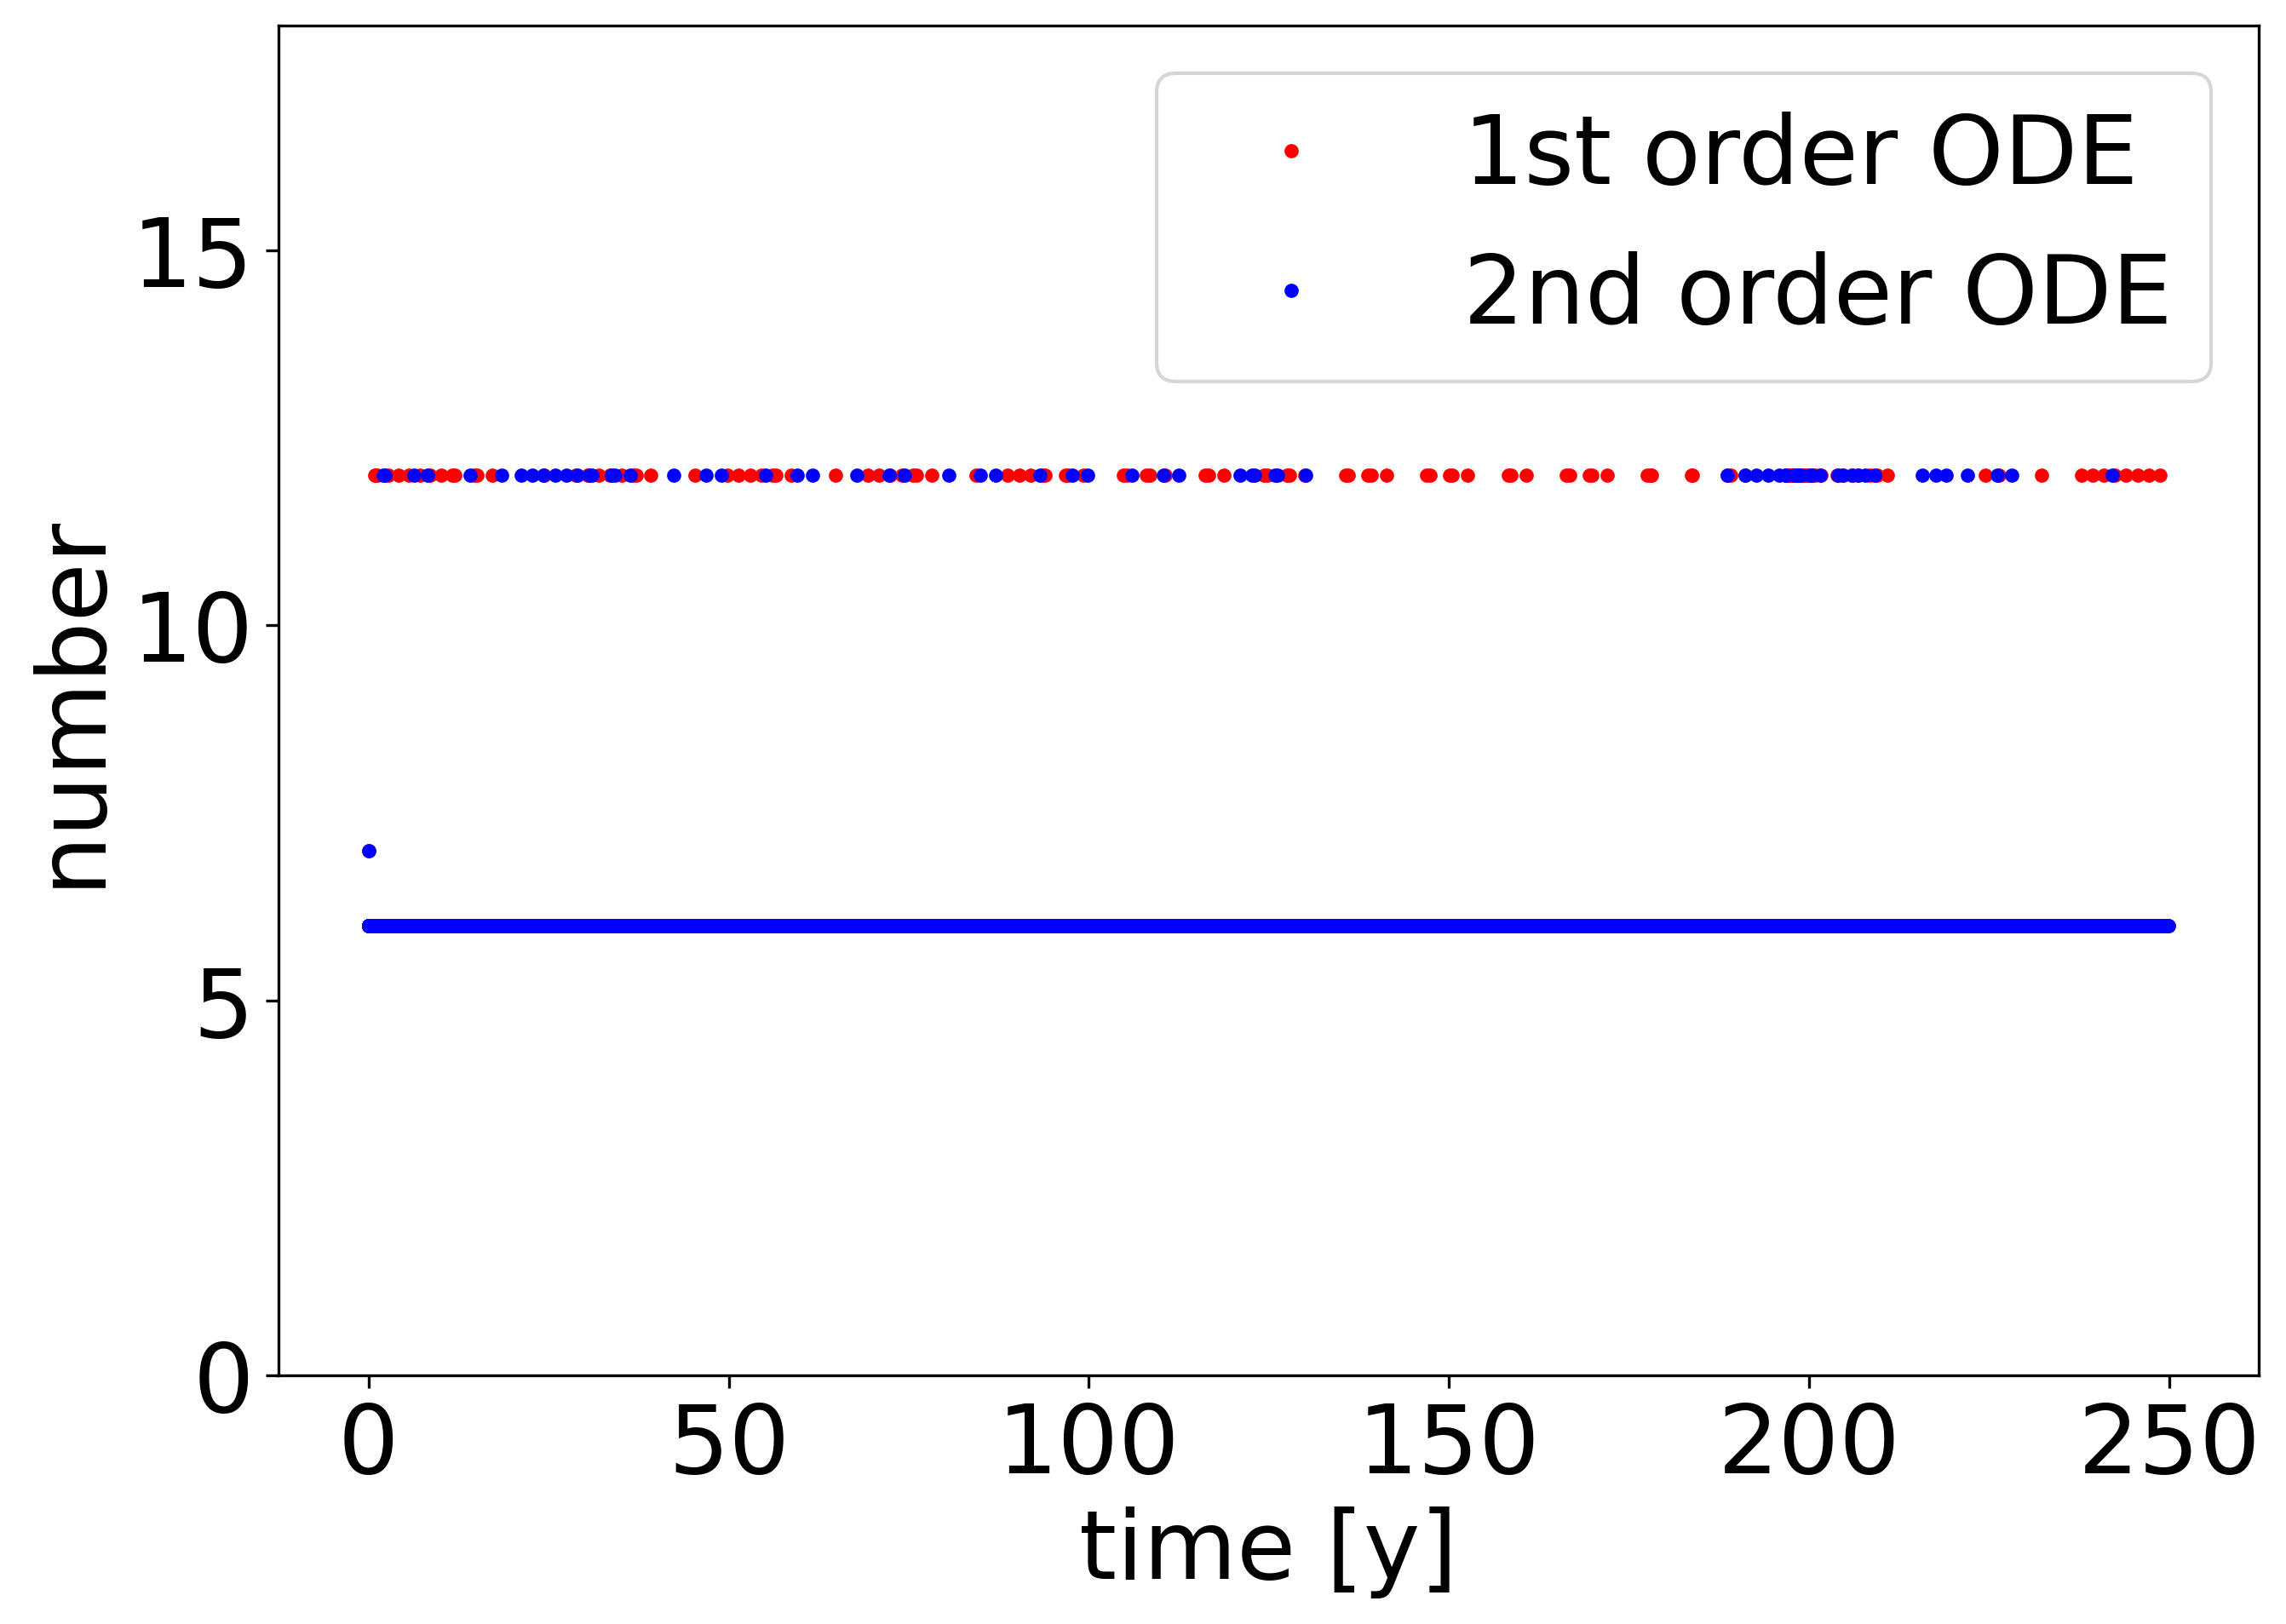
\includegraphics[width=1\textwidth]{images/TANDEMcompareFormulationstimeEvolutionRHSall.png}
       	\subcaption{Full simulation time} 
    \end{subfigure}
    \begin{subfigure}{0.32\textwidth}
    	\centering
    	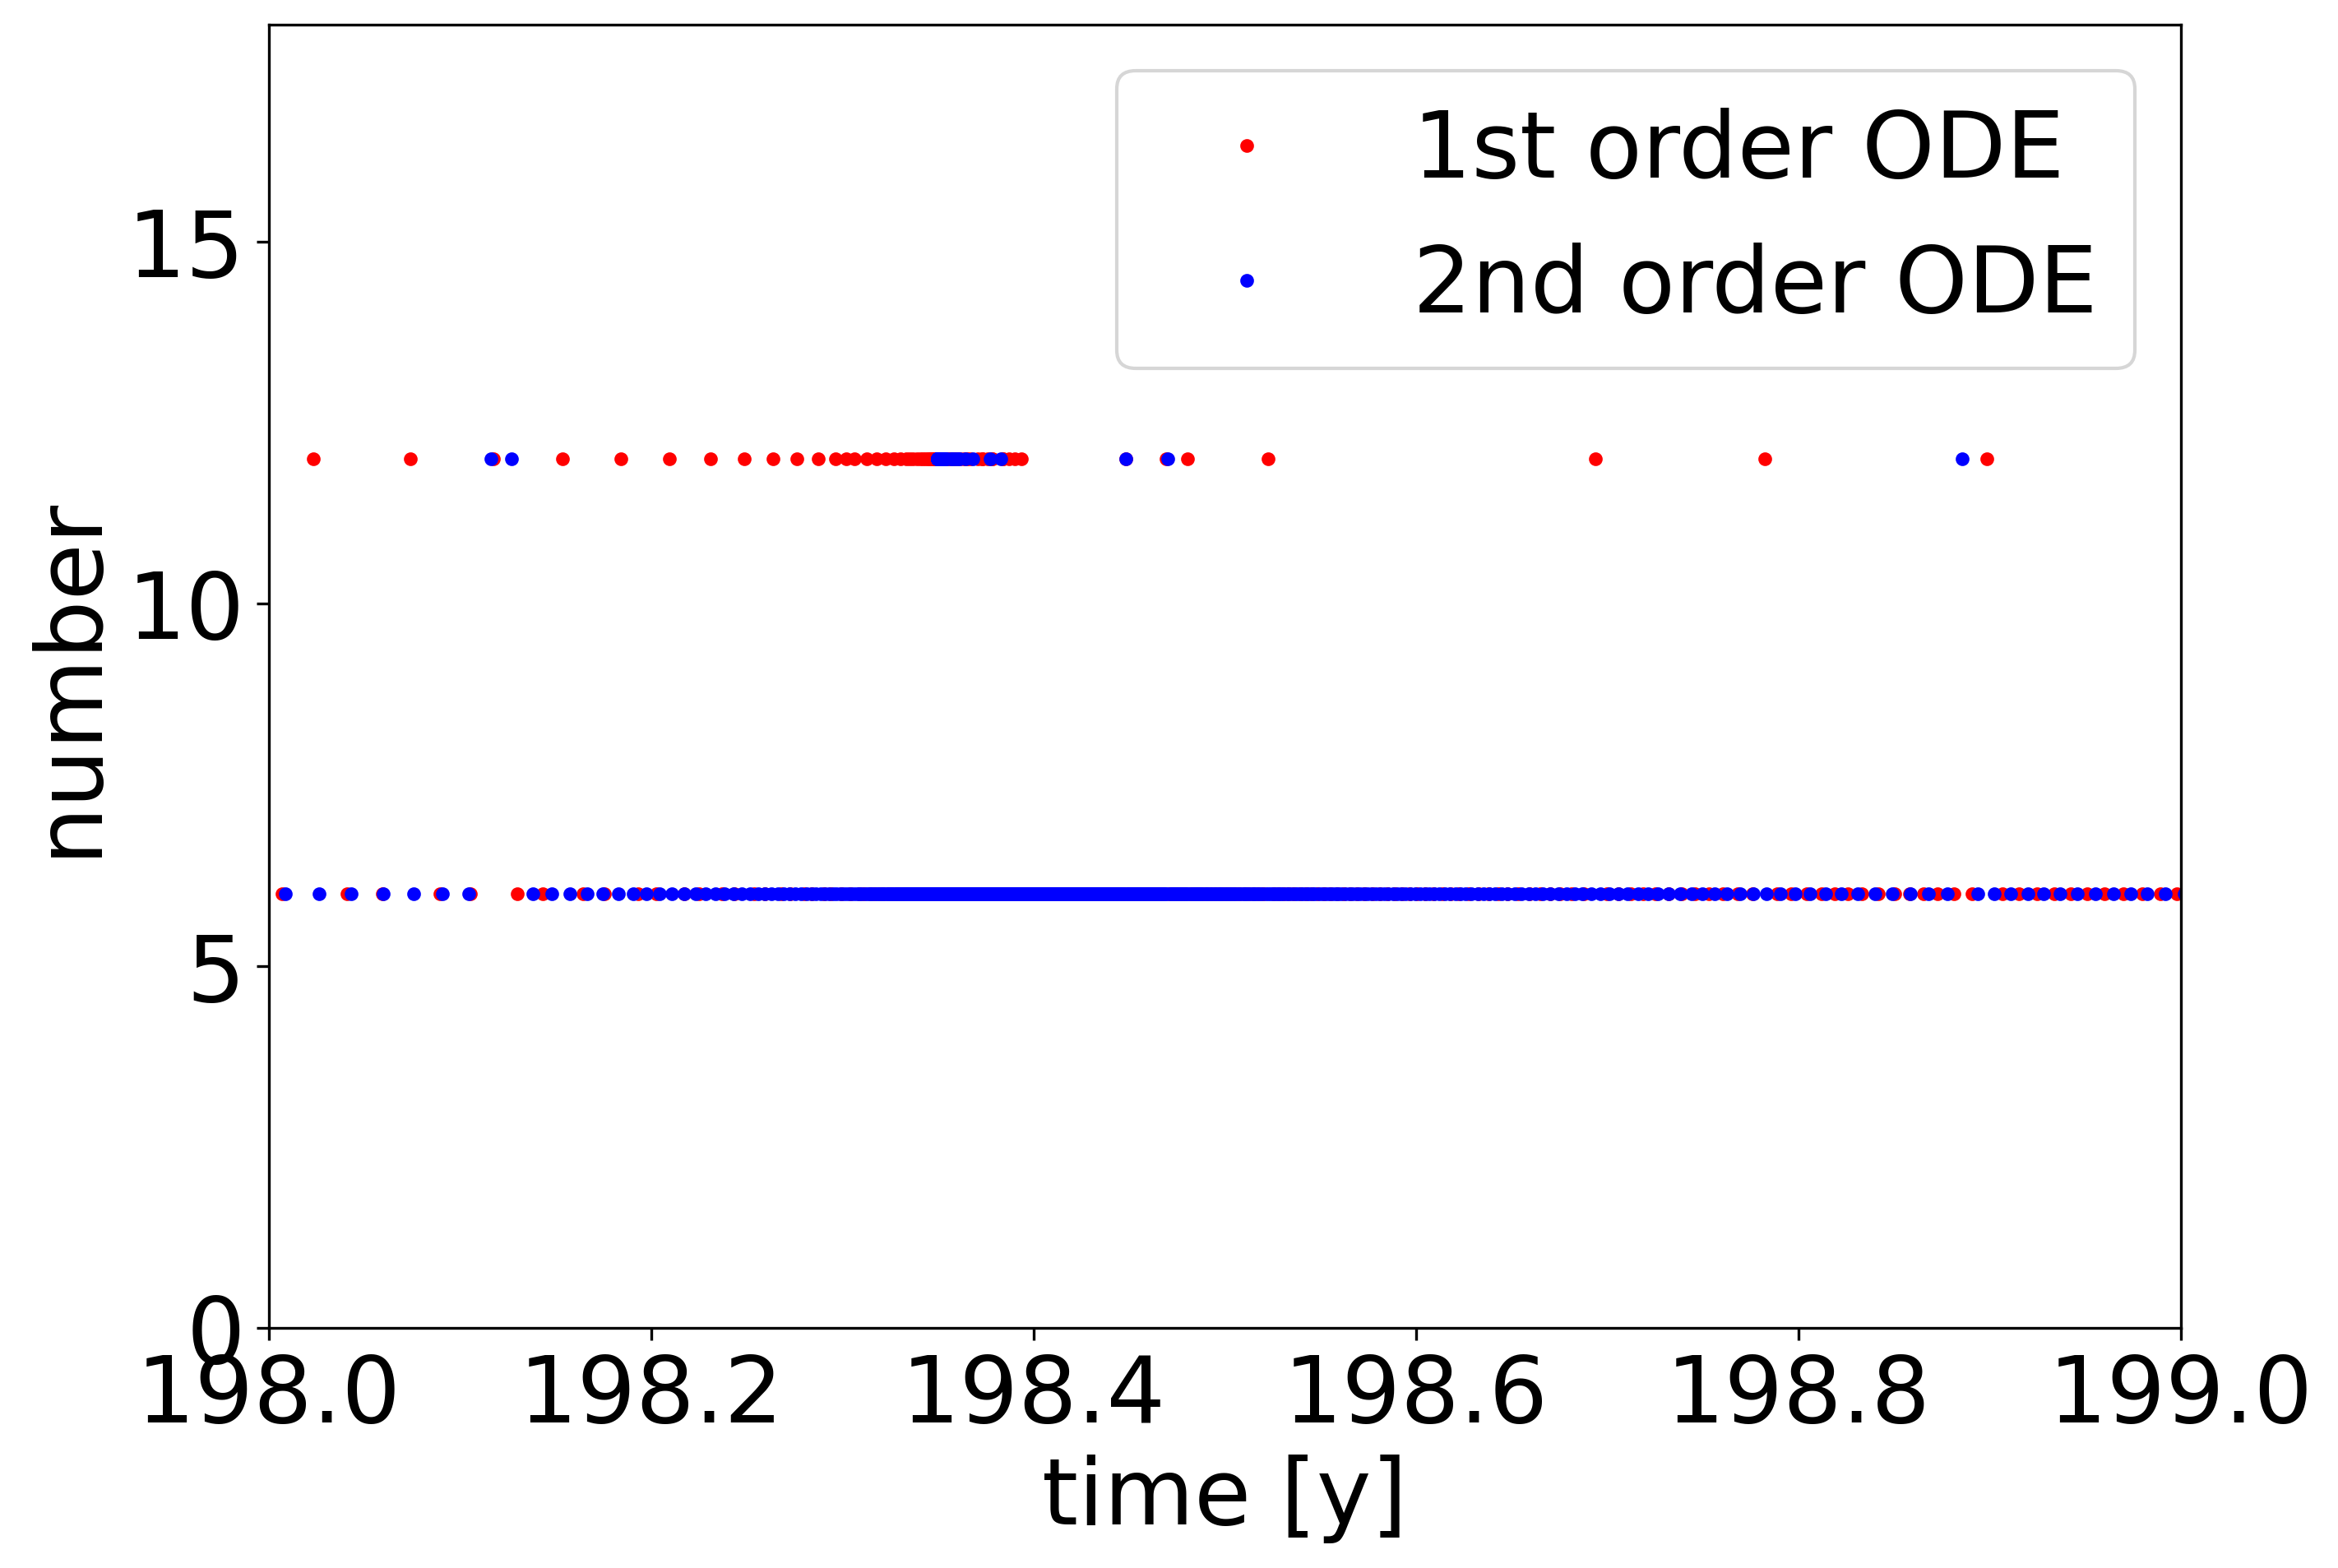
\includegraphics[width=1\textwidth]{images/TANDEMcompareFormulationstimeEvolutionRHSsurroundings.png}
       	\subcaption{Year of the earthquake} 
    \end{subfigure}
    \begin{subfigure}{0.32\textwidth}
    	\centering
    	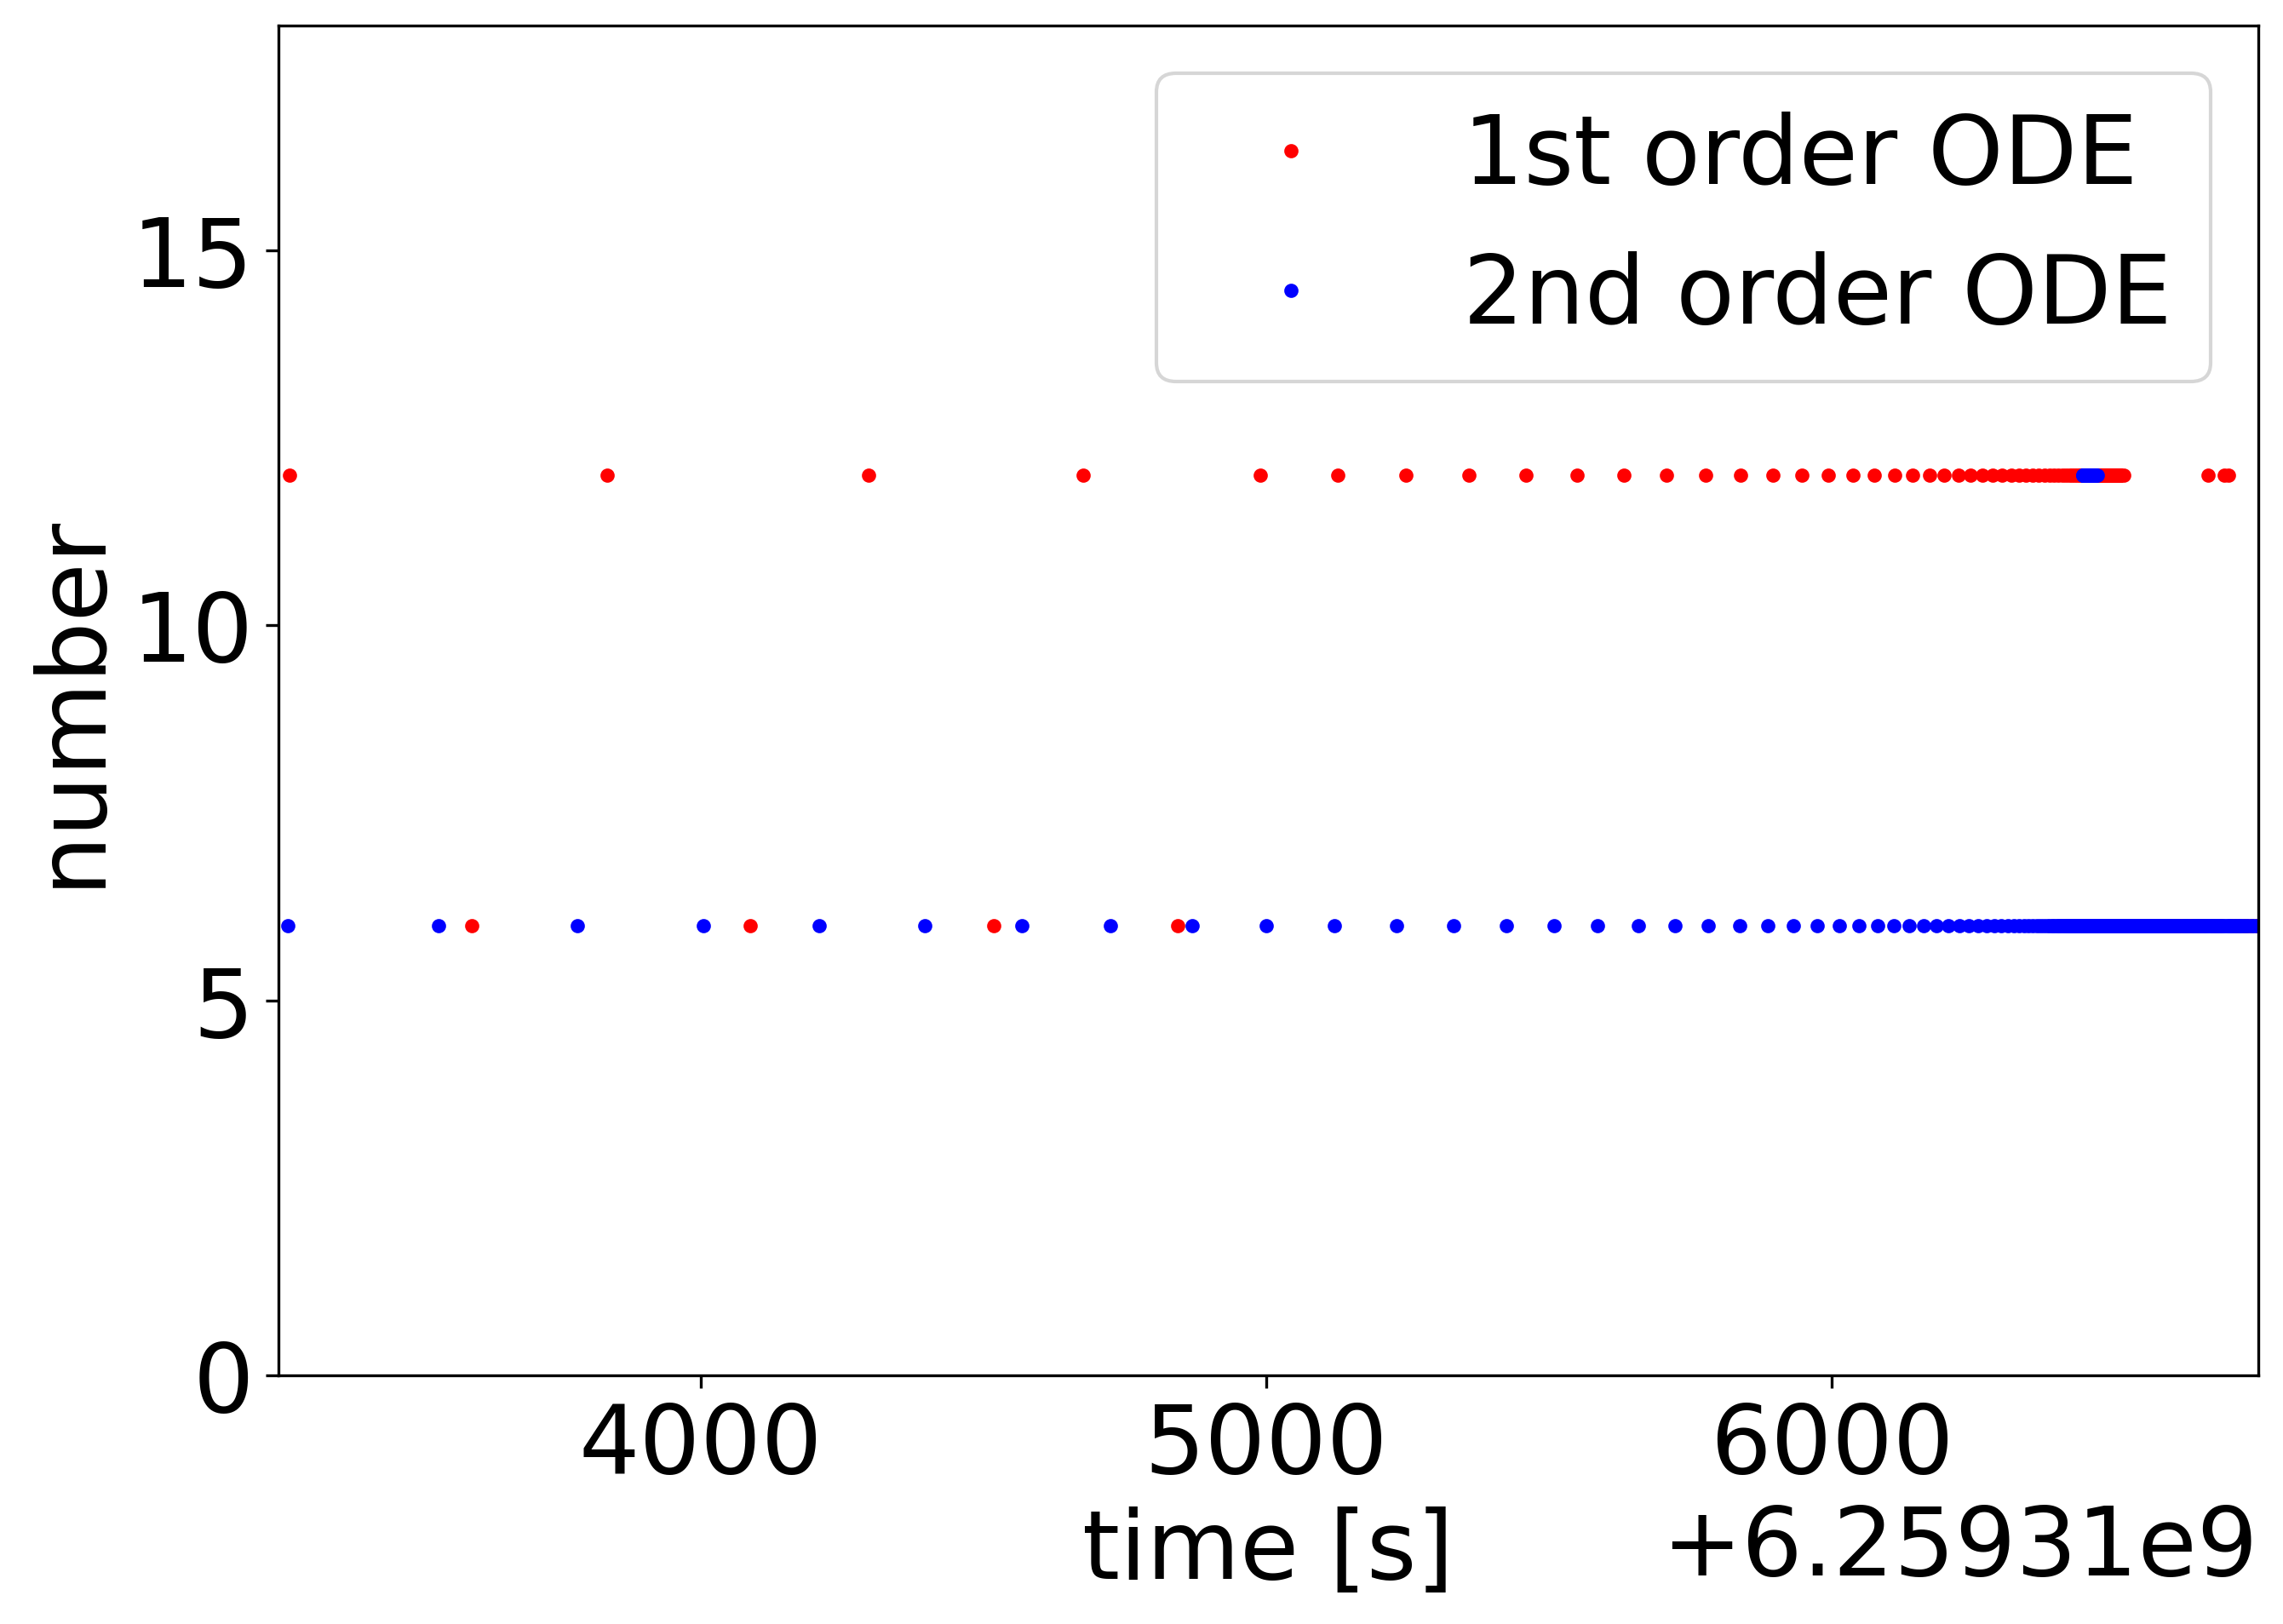
\includegraphics[width=1\textwidth]{images/TANDEMcompareFormulationstimeEvolutionRHSearthquake.png}
       	\subcaption{Evolution of the earthquake event} 
    \end{subfigure}
    \caption{Number of evaluations of the right hand side of the ODE in each time iteration for different solvers on the symmetric two-dimensional BP1 problem with 200 elements on the fault \newline
    \textbf{Legend:} \textcolor{red}{---} 1st order ODE formulation, \textcolor{blue}{---} 2nd order ODE formulation, \textcolor{green}{---} extended DAE formulation, \textcolor{yellow}{---} compact DAE formulation }
    \label{fig:timeEvolutionTANDEM_RHS}
\end{figure}

\section{Relative and Absolute Tolerances}
--> put that in the numerics section

\subsection{Behaviour of the Error}
Tolerances play a crucial role fort adaptive time-stepping methods. A proposed timestep is accepted only if the estimated error is inferior to a defined tolerance $t$, therefore a carefully chosen tolerance has a direct impact on the timestep size and consequently on the total number of time iterations to reach the final simulation time. If $u_i$ refers to all components of the solution vector and $u_i^{(e)}$ to the components of the embedded solution used for the error estimate, then a step is acceptable if following condition is fulfilled: 
\begin{equation}
    \left\|\frac{u_i - u_i^{(e)}}{t_i}\right\|_\infty = \max_i \left|\frac{u_i - u_i^{(e)}}{t_i}\right|
    \quad \leq \quad 1
\end{equation}
The infinity norm is used because a too large deviation in one node of the fault can erroneously provoke an earthquake at a too early time and thus strongly affects the accuracy of the results for the whole system. If the 2-norm was used, as it is common for other applications, too large errors at some nodes may occur, which are then compensated by nodes where the actual and the embedded solutions match well. \\
The tolerance $t_i$ can be defined independently for each component of the solution vector. It is calculated for each time step with an absolute tolerance $t_i^a$ and a relative tolerance $t_i^r$. 
\begin{equation}
    t_i = t_i^a + \max\left(u_i,u_i^{(e)}\right)t_i^r
\end{equation}
Since some components of the solution vector correspond to the values of the state variable $\psi$ and the other components correspond to the slip $S$, it is appropriate to use two different tolerances for the respective quantities. Thus, $t_i^a$ and $t_i^r$ take the values $t_\psi^a$ and $t_\psi^r$ in case the component at index $i$ refers to the state variable and the values $t_S^a$ and $t_S^r$ if the index $i$ refers to the slip at the fault. The motivation behind this decision can be seen in \autoref{fig:errrors1e-7}, which depicts the maximal absolute and relative errors ($\max_i\left|u_i-u_i^{(e)}\right|$ and $\max_i\left|\frac{u_i-u_i^{(e)}}{u_i}\right|$) for the respective components of $\psi$ and $S$. For this simulation, all errors have been set to $t_i^r = t_i^a = 10^{-7}$, without any distinction between slip or state variable components nor between relative or absolute tolerances.
\begin{figure}[H]
    \centering
    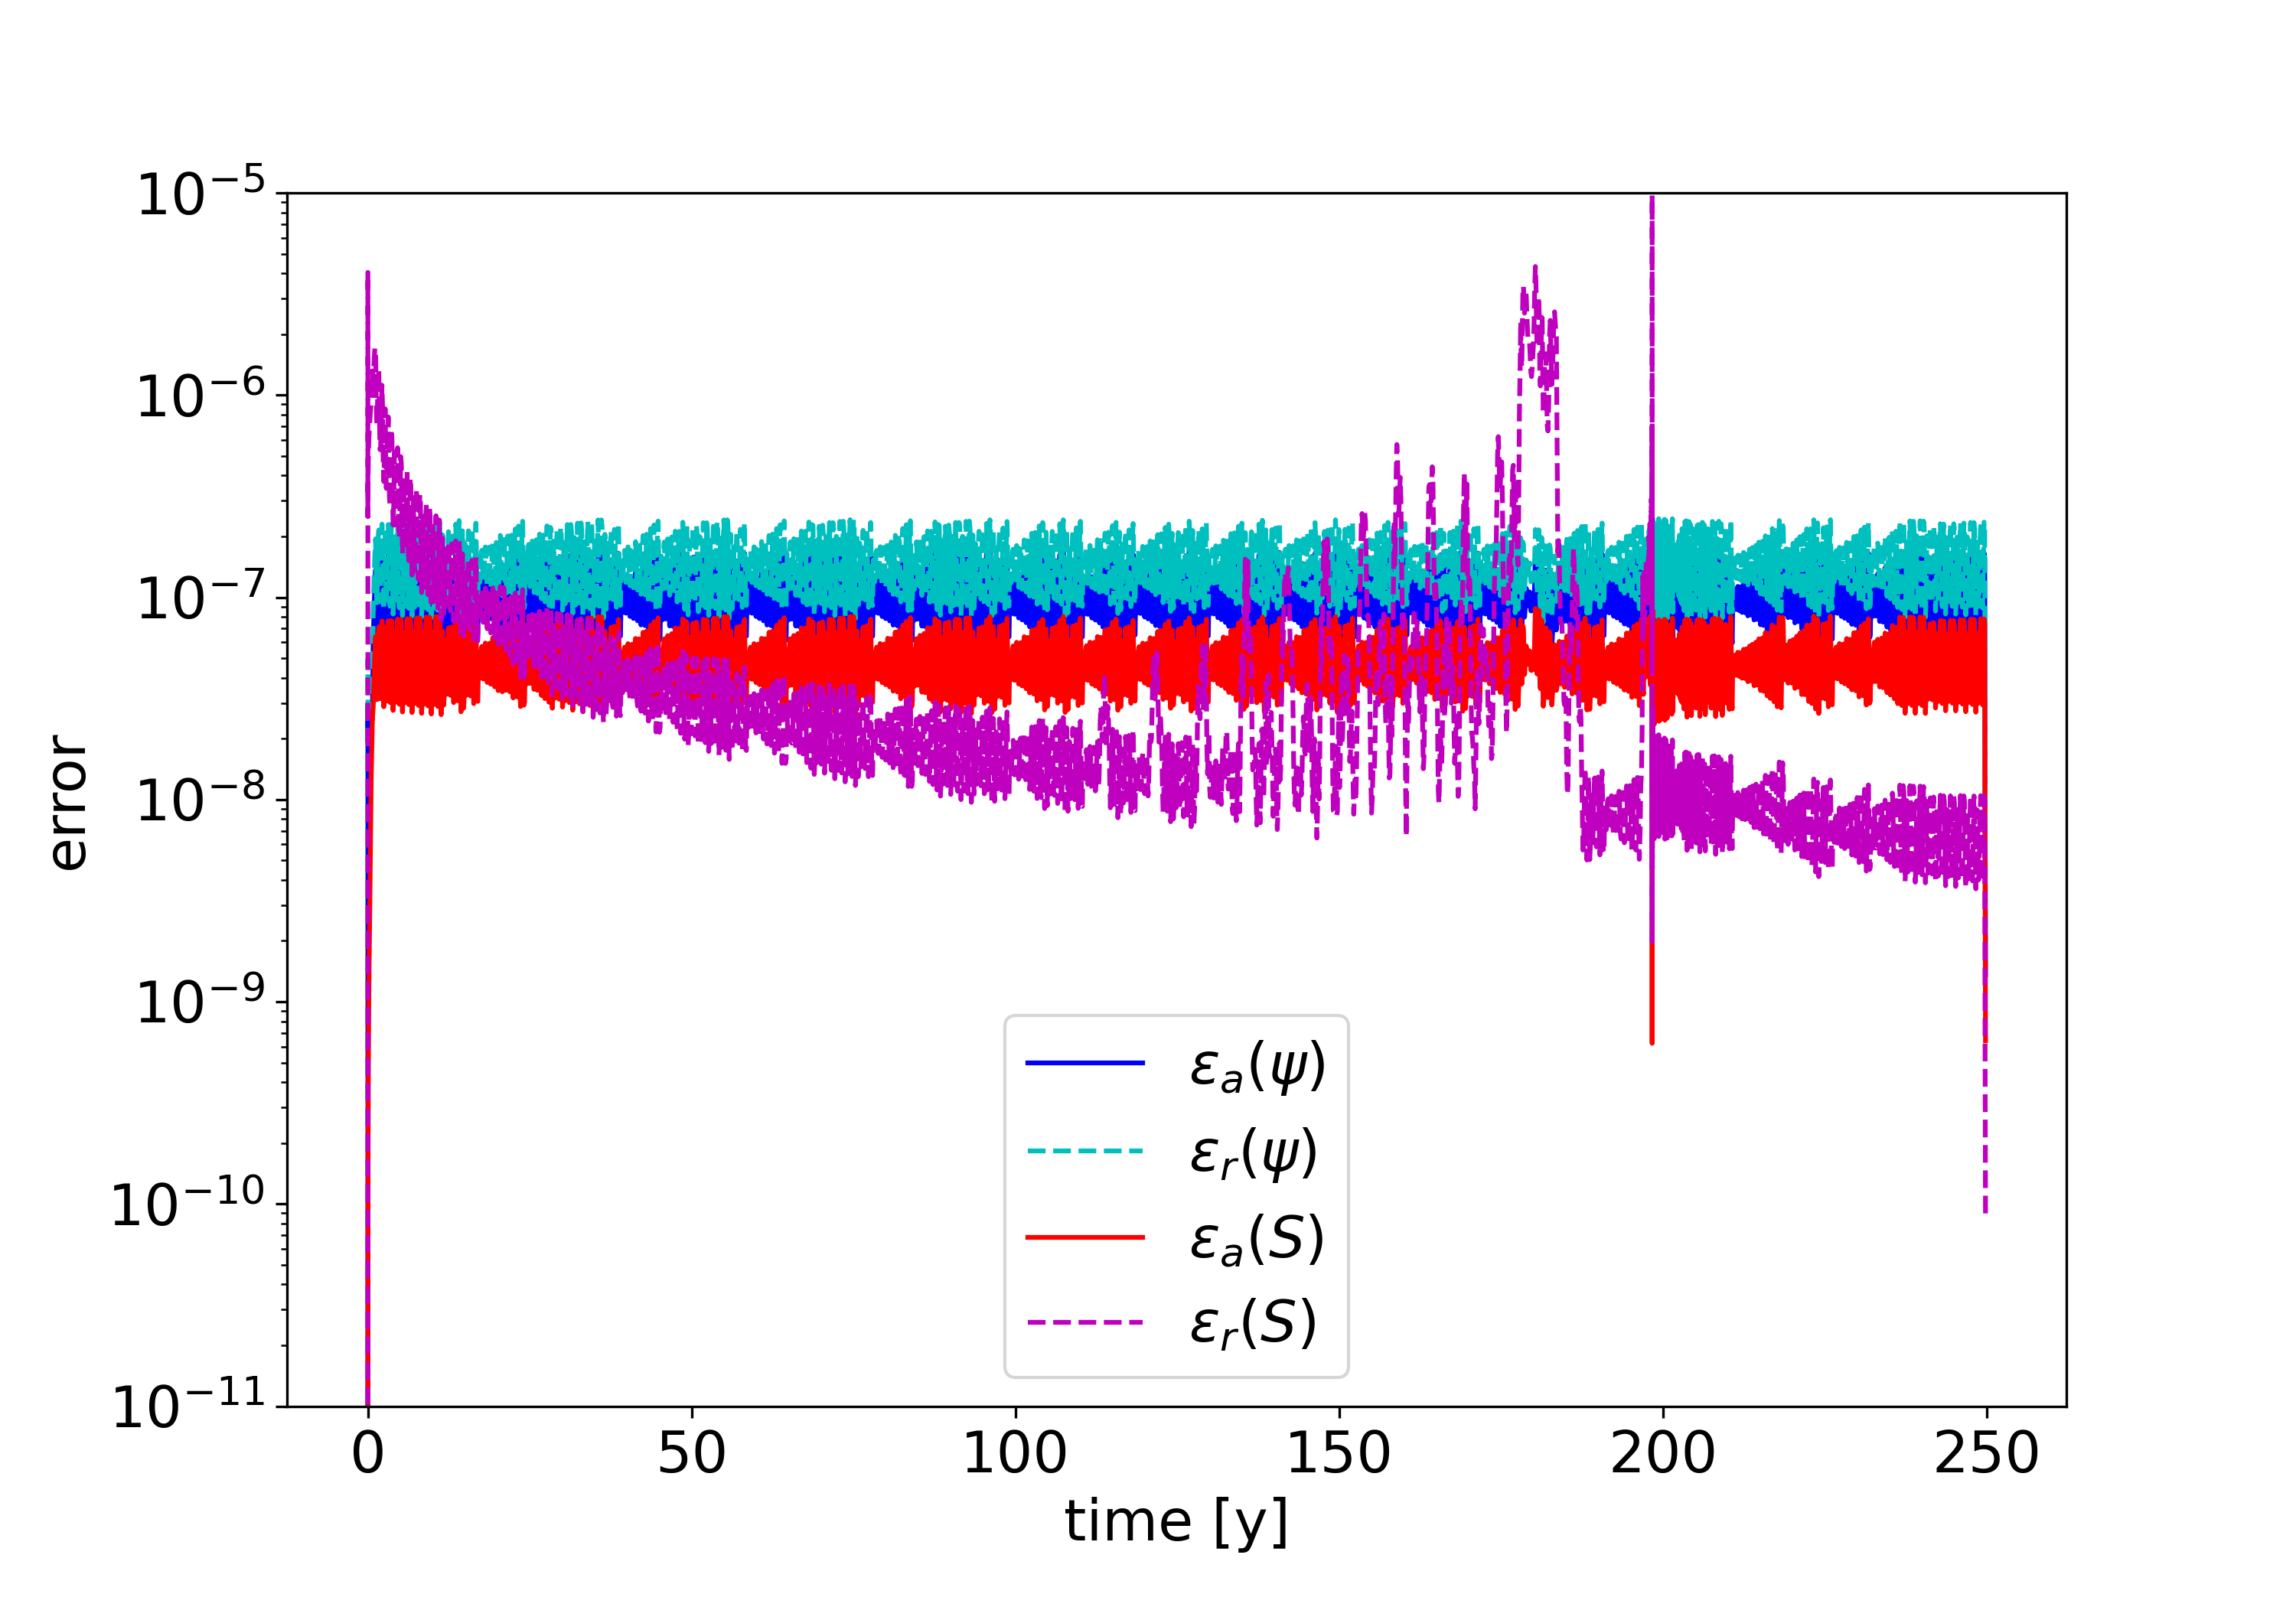
\includegraphics[width=0.6\textwidth]{images/TANDEMtimeEvolutionErrorall_RKDP5.png}
    \caption{Maximum relative and absolute errors using the RKDP5 method on a fault with 200 elements with an absolute and relative error tolerance of $10^{-7}$}
    \label{fig:errrors1e-7}
\end{figure}
Over the whole simulation time, the state variable $\psi$ takes values close to $0.8$ on all fault nodes, leading to a total tolerance for the corresponding components of $t_\psi \approx 1.8 \cdot 10^{-7}$. The blue line, which draws the maximum absolute error, is clearly limited by this tolerance value and the light blue line of the relative error is located, as expected, by a factor $1/0.8$ above the absolute error. \\
The error analysis of the slip presents a much less regular picture. The maximal absolute error lies always below the tolerance $t_S^a = 10^{-7}$, however the relative error reaches much higher values at the beginning of the simulation and before the earthquake event. The evolution of the extreme values of the slip in \autoref{fig:minmax1e-7} provides an explanation for these large errors. In the beginning, the slip at each node is below 1, thus the overall tolerance \\

\begin{figure}[H]
    \centering
    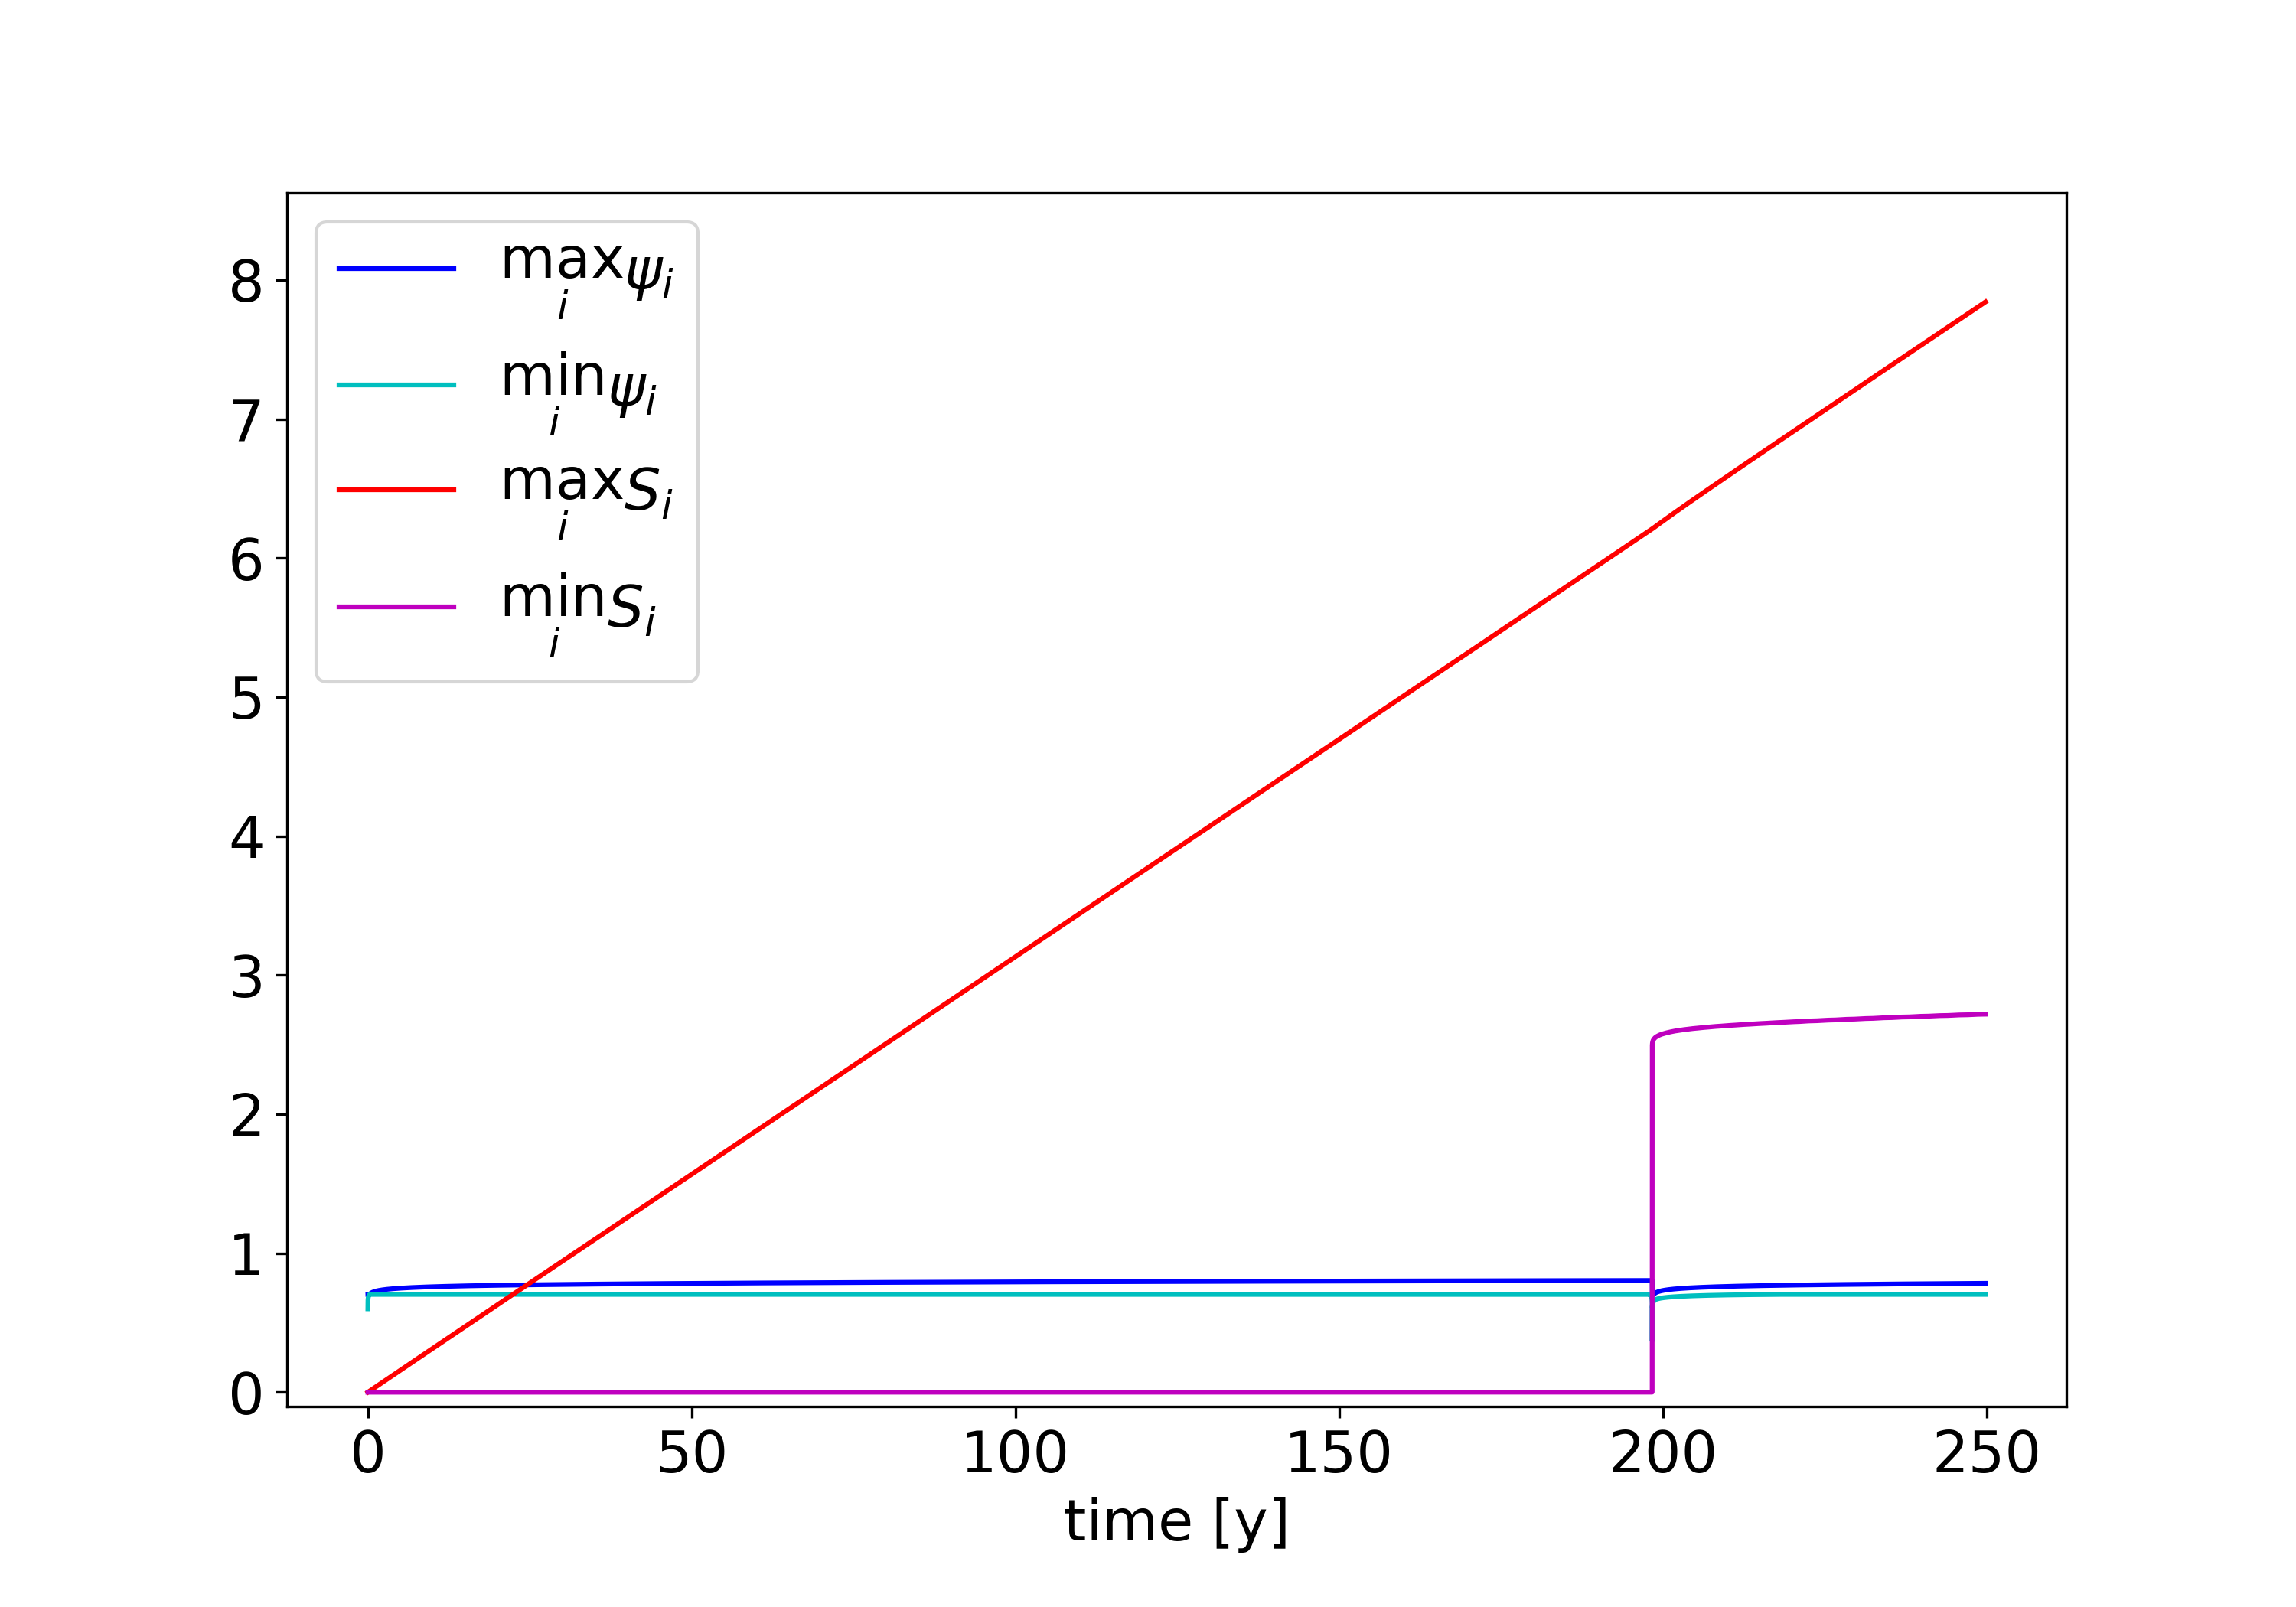
\includegraphics[width=0.6\textwidth]{images/TANDEMtimeEvolutionMinMaxAll_RKDP5.png}
    \caption{Maximum and minimum values of the state variable $\psi$ and of the slip $S$ over time. Simulation performed with the RKDP5 method on a fault with 200 elements with an absolute and relative error tolerance of $10^{-7}$}
    \label{fig:minmax1e-7}
\end{figure}

\subsection{Tolerance of the State Variable Dependent on the Slip}
Overall, the absolute error of the slip is inferior to the absolute error of the state variable. From a physical point of view, the slip is a relevant quantity to describe earthquakes whereas the state variable $\psi$ is only required to solve the DAE. Therefore, the absolute and relative tolerances are defined as external requirements for the slip only, and the tolerances for the state variable have to be chosen in a way to achieve the best numerical performance without loosing physical accuracy. In the following equations, we try to evaluate the highest acceptable tolerances for the state variable in function of the provided tolerances for the slip. The relation between $S$ and $\psi$ is described by the friction law in \autoref{eq:SEASDAE_frictionLaw}, which is evaluated at a constant velocity $V^*$. For a maximal absolute slip error $\epsilon_S^a$, the largest acceptable absolute error of the state variable $\epsilon_\psi^a$ can be calculated by equalizing the induced error in the friction law under constant velocity. 
\begin{align}
    f_{V^*}(S+\epsilon_S^a,\psi) - f_{V^*}(S,\psi) &= f_{V^*}(S,\psi+\epsilon_\psi^a) - f_{V^*}(S,\psi) \\
    \tau(U(S+\epsilon_S^a)) - \tau(U(S)) &= a \sigma_n \text{arsinh}\left(\frac{V^*}{2V_0}\right)\frac{1}{a}\left(e^{\frac{\psi+\epsilon_\psi^a}{a}} - e^{\frac{\psi}{a}}\right) \\
    \tau(B(S+\epsilon_S^a)) - \tau(BS) &= a \sigma_n \text{arsinh}\left(\frac{V^*}{2V_0}\right) e^{\frac{\psi}{a}}\left(e^{\frac{\epsilon_\psi^a}{a}} - 1\right)
\end{align}

As already discussed in the formulation of the Jacobian matrix, the displacement $U(S)$ is linear in $S$ and can therefore be expressed with the linear transformation matrix $B$ as $U(S) = BS$. Further transformations of the left side of the equation are performed in index notation, where $\mathbbm{1}$ denotes a vector in which all components are equal to one. 
\begin{align}
    (\nabla u(S))_{pq} =& \frac{1}{2}\left(D_{lpq}^0u_l^0 + D_{lpq}^1u_l^1\right) + c_0\left(E_{lq}^0u_l^0 - E_{lq}^1u_l^1 - f_q\right)n_{pq} \\ \nonumber
    (\nabla u(S + \epsilon_S^a))_{pq} =& \frac{1}{2}\left(D_{lpq}^0\left(u_l^0+ B_{lj}\mathbbm{1}_j\epsilon_S^a\right) + D_{lpq}^1\left(u_l^1+ B_{lj}\mathbbm{1}_j\epsilon_S^a\right)\right) \\ &+ c_0\left(E_{lq}^0\left(u_l^0+ B_{lj}\mathbbm{1}_j\epsilon_S^a\right) - E_{lq}^1\left(u_l^1+ B_{lj}\mathbbm{1}_j\epsilon_S^a\right) - f_q\right)n_{pq} \\
    (\nabla u(S + \epsilon_S^a))_{pq} - (\nabla u(S))_{pq} =& \left(\frac{1}{2}\left(D_{lpq}^0 + D_{lpq}^1\right) + c_0\left(E_{lq}^0 - E_{lq}^1\right)n_{pq}\right)B_{lj}\mathbbm{1}_j\epsilon_S^a \\
    \tau_p(B(S+\epsilon_S^a)) - \tau_p(BS) =& M_{rp}^{-1}e_{qr}^Tw_q\left((\nabla u(S + \epsilon_S^a))_{kq} - (\nabla u(S))_{kq}\right)n_{kq}
\end{align}
We can see that the error in $\tau$ does not depend on the slip $S$ anymore and is proportional to the absolute slip error $\epsilon_S^a$. We can thus define a matrix $C$ such that $\tau_p(B(S+\epsilon_S^a)) - \tau_p(BS) = C_{pj}\mathbbm{1}_j\epsilon_S^a$. The absolute error of the state variable is then directly proportional to $\epsilon_S^a$. 
\begin{align}
    \epsilon_\psi^a &= a\text{ln}\left(1+\frac{C_{pj}\mathbbm{1}_j}{a\sigma_n \text{arsinh}\left(\frac{V^*}{2V_0}\right)e^{\frac{\psi}{a}}}\epsilon_S^a\right) 
\end{align}
To provide an upper bound for $\epsilon_\psi^a$, the smallest value of the proportionality factor of $\epsilon_S^a$ has to be determined because the logarithm function is increasing and the smallest allowed value of the error is searched. For the numerator of the ratio, to calculate $\min_p\left|C_{pj}\mathbbm{1}_j\right|$ minimizes the ratio. Note that the matrix $C$ depends on the geometry so this term cannot be provided in general in beforehand but has to be chosen with respect to the used space discretization. To minimize the ratio, the terms on the denominator have to be maximized. Because the arsinh function increases monotonously, the choice of $V_{max}$ for the velocity component provides an appropriate upper bound. Similarly, $\psi$ should be replaced by an upper limit $\psi_{max}$. The value of the parameter $a$ depends on the fault location and varies between $a_{min}$ and $a_{max}$. It appears once at the beginning of the denominator, where its maximal value shall be chosen, and once in the exponential, where its minimal value is required. If all those values are plugged into the expression, the error in $\psi$ can be evaluated as following: 
\begin{equation}
    \epsilon_\psi^a = a_{min}\text{ln}\left( 1+\frac{\min_p\left|C_{pj}\mathbbm{1}_j\right|}{a_{max}\sigma_n \text{arsinh}\left(\frac{V_{max}}{2V_0}\right) e^{\frac{\psi_{max}}{a_{min}}}}\epsilon_S^a\right)
\end{equation}
The upper bounds for the velocity and for the state variable can be deduced by already obtained simulation results and an appropriate choice could be the values $V_{max} = 5.0ms^{-1}$ and $\psi_{max} = 0.85$. In the simulation settings, $a$ increases from $a_{min}=0.010$ at the surface to $a_{max}=0.025$ at high depths. With these values, all terms take reasonable values, except for the exponential $e^{\frac{\psi_{max}}{a_{min}}} = e^{85} \approx 8\cdot10^{36}$. In the vicinity of 1,  the logarithm can be approximated by a linear function with gradient 1. Under consideration of the initial factor $a_{min}$, the absolute error tolerance in $\psi$ has to be 38 magnitudes below the tolerance in the slip to prevent any additional error. Such a low tolerance is not achievable in any realistic scenario, so the state variable participates in making the simulation less accurate. When the tolerances for the state variable have to be set, and only an absolute tolerance for the slip is provided, it is the best to chose them as low as possible, and still the state variable will contribute to the error of the simulation. On the other hand, very low tolerances prevent the choice of larger timesteps and an appropriate choice of the tolerance for the state variable which is not too low to ensure reasonable execution times still needs to be determined.  

\subsection{Tolerance of the State Variable Dependent on the Slip Rate}
So far, the error in the slip rate $V$ is not directly regulated by any tolerance value. Since it is calculated from the slip and from the state variable, the error in $V$ depends on the chosen tolerances for those two parameters. As a physical quantity, it might be interesting to provide a tolerance for the slip rate too. Unlike for the slip, the tolerance for the slip rate should also include a relative error tolerance $t_V^r$ in addition to the already discussed absolute error tolerance $t_V^a$. Indeed, the slip rate takes values around $10^{-6}ms^{-1}$ in the aseismic phase and peaks at values above $10^{9}ms^{-1}$ during the earthquake event. The exclusive use of an absolute error tolerance, with a value below the slip rate of the aseismic evolution, is too restrictive during the earthquake. An appropriate relative error tolerance, which is scaled by the current velocity value and added to the absolute one can reasonably restrict the error. In the aseismic phase, the relative error tolerance does not have much effect since it is scaled down by the very low slip rate and outmatched by the presumably higher absolute tolerance. For example, the choices $t_V^a=10^{-10}$ and $t_V^r=10^{-7}$ allow for a relative error of the order $10^{-4}$ during the aseismic phase and of the order $10^{-7}$ during the earthquake. Such a choice reflects the concept that a higher accuracy is needed to simulate an earthquake than to simulate aseismic slip. \\
The typical approach would be to estimate it with the difference between the values obtained from the numerical solution and its embedded solution. The newly chosen timestep shall then only allow solutions which fulfill the tolerances in the entire state vector and the additional tolerance in error of the slip rate. Alternatively, the error tolerance of the state variable, which is not properly defined from physical constrains yet can be used to restrict the slip rate. To obtain the relation between error in slip rate $V$ and state variable $\psi$, the same analysis as in the previous subsection has to be performed. This time, the error in the friction law is evaluated under the assumption of a constant slip $S^*$.  
\begin{align}
	f_{S^*}(V+\epsilon_V^a,\psi) - f_{S^*}(V,\psi) &= f_{S^*}(V,\psi+\epsilon_\psi^a) - f_{S^*}(V,\psi) \\
	 f_{S^*}(V,\psi) + \frac{d}{dV}f_{S^*}(V,\psi)\epsilon_V^a - f_{S^*}(V,\psi) + \mathcal{O}\left(\left(\epsilon_V^a\right)^2\right)&= a \sigma_n \text{arsinh}\left(\frac{V}{2V_0}\right)\frac{1}{a}\left(e^{\frac{\psi+\epsilon_\psi^a}{a}} - e^{\frac{\psi}{a}}\right) \\
	 \left( \frac{a\sigma_ne^{\frac{\psi}{a}}} {2V_0\sqrt{\left(\frac{V}{2V_0}\right)^2+1}}- \eta \right)\epsilon_V^a + \mathcal{O}\left(\left(\epsilon_V^a\right)^2\right) &= a \sigma_n \text{arsinh}\left(\frac{V}{2V_0}\right) e^{\frac{\psi}{a}}\left(e^{\frac{\epsilon_\psi^a}{a}} - 1\right)
\end{align}
\begin{equation}
	 \epsilon_\psi^a 
	= a\text{ln}\left(1 + \left( \frac{1}{\text{arsinh}\left(\frac{V}{2V_0}\right)\sqrt{V^2 + (2V_0)^2}} - \frac{\eta}{a \sigma_n \text{arsinh}\left(\frac{V}{2V_0}\right) e^{\frac{\psi}{a}}} \right)\epsilon_V^a + \mathcal{O}\left(\left(\epsilon_V^a\right)^2\right)\right)
\end{equation}
The exponential $e^{\frac{\psi}{a}}$ with the extremely high value appears again in one of the two ratios. The term with $\eta$ can thus be neglected to estimate the error. In the remaining summand, an appropriate estimate value for the slip rate $V$ needs to be determined. As stated previously, the absolute error tolerance is only relevant for the aseismic phase, in which the slip rate never exceeds the tectonic slip $V_0$, which can be taken as an upper bound for the slip rate here. The absolute error is then calculated by: 
\begin{equation}
	\label{eq:absoluteErrorPSIFromV}
	 \epsilon_\psi^a 
	= a_{min}\text{ln}\left(1 +  \frac{1}{\text{arsinh}\left(\frac{1}{2}\right)\sqrt{5}V_0}\epsilon_V^a\right)
\end{equation}
During an earthquake, the relative error tolerance of the slip rate is relevant. To evaluate it, we now investigate the relation between the relative errors of the slip rate and the state variable. 
\begin{align}
	f_{S^*}((1+\epsilon_V^r)V,\psi) - f_{S^*}(V,\psi) &= f_{S^*}(V,(1+\epsilon_\psi^r)\psi) - f_{S^*}(V,\psi) \\
	f_{S^*}(V,\psi) + \frac{d}{dV}f_{S^*}(V,\psi)\epsilon_V^rV - f_{S^*}(V,\psi) + \mathcal{O}\left(\left(\epsilon_V^rV\right)^2\right)&= a \sigma_n \text{arsinh}\left(\frac{V}{2V_0}\right)\frac{1}{a}\left(e^{\frac{(1+\epsilon_\psi^r)\psi}{a}} - e^{\frac{\psi}{a}}\right) \\
	\left( \frac{a\sigma_ne^{\frac{\psi}{a}}} {2V_0\sqrt{\left(\frac{V}{2V_0}\right)^2+1}}- \eta \right)\epsilon_V^rV + \mathcal{O}\left(\left(\epsilon_V^rV\right)^2\right) &= a \sigma_n \text{arsinh}\left(\frac{V}{2V_0}\right) e^{\frac{\psi}{a}}\left(e^{\frac{\epsilon_\psi^r}\psi{a}} - 1\right)
\end{align}
\begin{equation}
	\epsilon_\psi^r = \frac{a}{\psi}\text{ln}\left(1 + \left( \frac{1}{\text{arsinh}\left(\frac{V}{2V_0}\right)\sqrt{V^2 + (2V_0)^2}} - \frac{\eta}{a \sigma_n \text{arsinh}\left(\frac{V}{2V_0}\right) e^{\frac{\psi}{a}}} \right)\epsilon_V^rV + \mathcal{O}\left(\left(\epsilon_V^rV\right)^2\right)\right)
\end{equation}
Again, the term with $\eta$ can be neglected because of the exponential. For elements, where the relative tolerance is relevant, the slip rate is much larger than the tectonic slip, so $V_0^2$ can also be neglected below the square root when added to $V^2$. The relative error in $\psi$ can be estimated as: 
\begin{equation}
	\label{eq:relativeErrorPSIFromV}
	\epsilon_\psi^r = \frac{a_{min}}{\psi_{max}}\text{ln}\left(1 + \frac{1}{\text{arsinh}\left(\frac{V_{max}}{2V_0}\right)}\epsilon_V^r\right)
\end{equation}

The absolute and relative errors in $\psi$ associated to the respective errors in the slip rate are represented in \autoref{fig:RelAbsErrorToleranceVPSI}. The curves show the evaluation of \autoref{eq:absoluteErrorPSIFromV} and \autoref{eq:relativeErrorPSIFromV} for small error values in $V$. The various parameters are set to $a_{min}=0.01$, $\psi_{max}=0.85$, $V_0=10^{-6}ms^{-1}$ and $V_{max}=5.0ms^{-1}$. To use the previous example again, if an absolute error tolerance in the slip rate of $t_V^a=10^{-10}$ and a relative tolerance of $t_V^r=10^{-7}$ are required, it would translate to the tolerances in the state variable to $t_\psi^a=9.29\cdot10^{-7}$ and $t_\psi^r=2.77\cdot10^{-11}$. However, these values cannot be used as such in the simulation, since the assumption that the absolute tolerance can be neglected during the earthquake and inversely that the relative tolerance is insignificant in the aseismic phase only holds for the slip rate but not for the state variable, whose value remains between $0.75$ and $0.85$. It makes more sense to define an absolute tolerance for the aseismic slip $t_\psi^{as}=9.29\cdot10^{-7}$ and for the earthquake $t_\psi^{eq}=\psi_{min}2.77\cdot10^{-11}=6.48\cdot10^{-11}$ in the state variable. 

\begin{figure}[H]
	\centering
	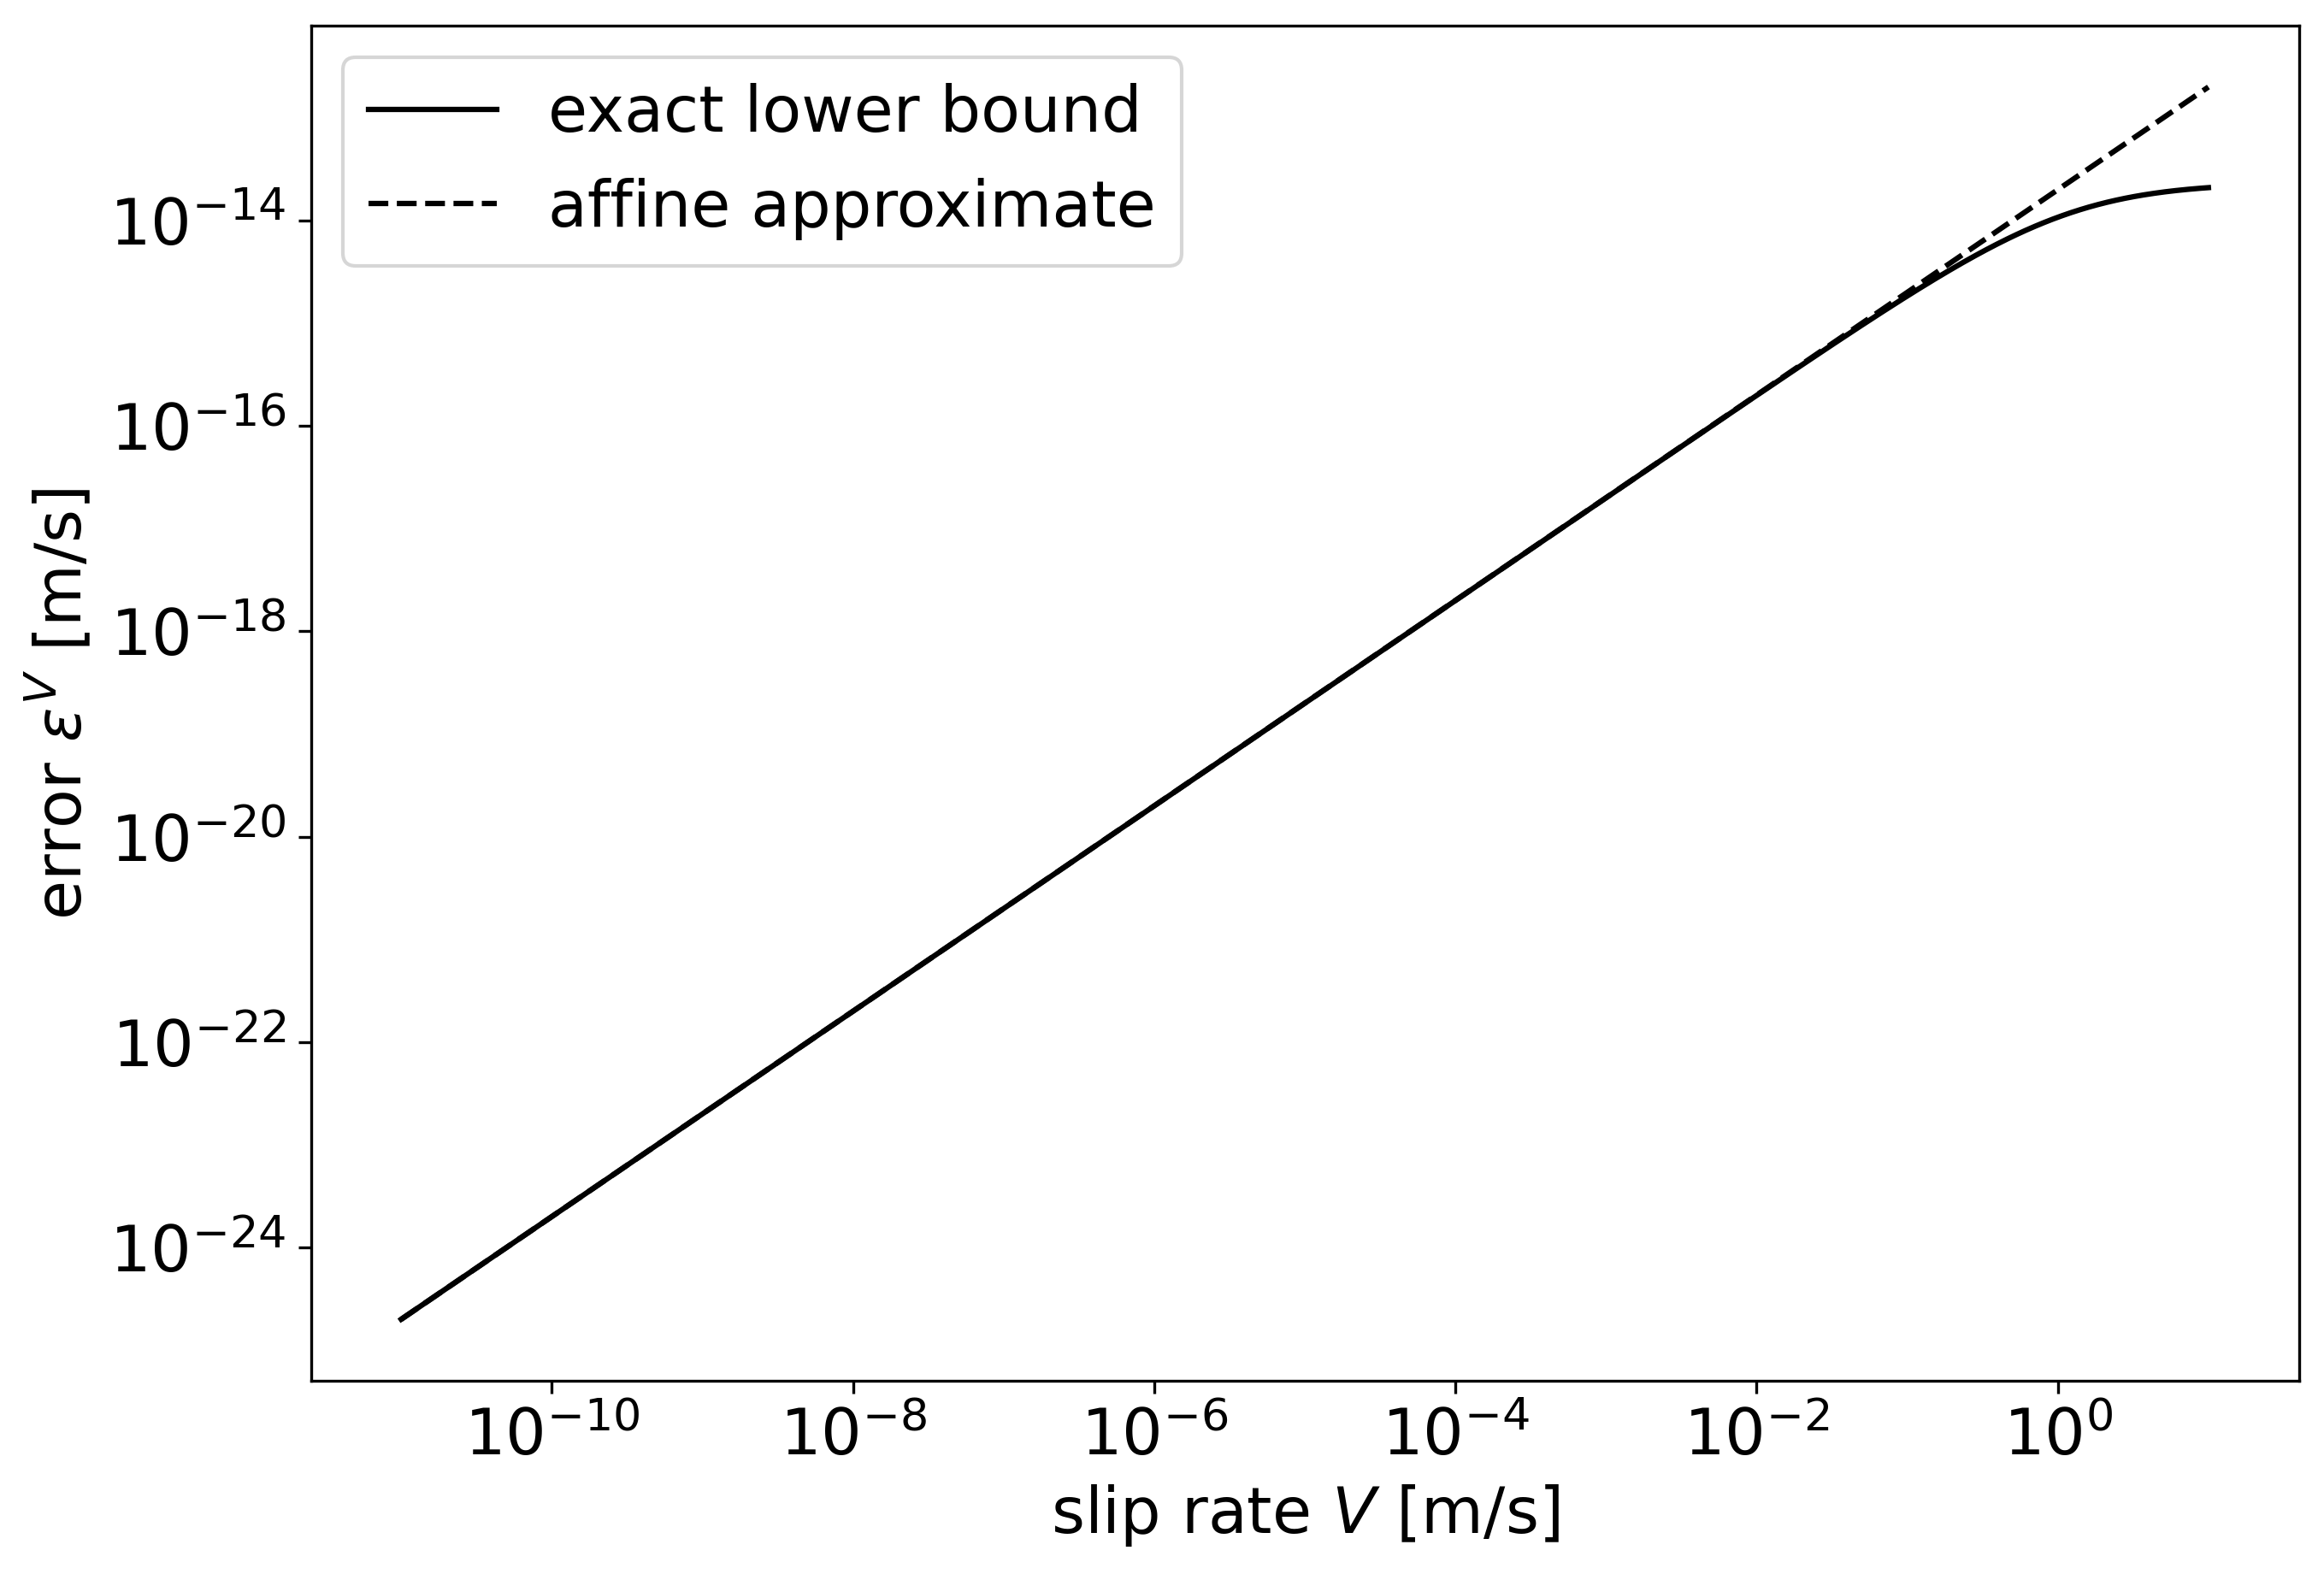
\includegraphics[width=0.6\textwidth]{images/ErrorRelationPSI_VAbsoluteRelative.png}
	\caption{Absolute and relative error in $\psi$ in function of the error in the slip rate}
	\label{fig:RelAbsErrorToleranceVPSI}
\end{figure}

\begin{equation*}
	F(x,y) = 0, y(x) \qquad x\in\mathbb{R}^n, y\in\mathbb{R}^m,F\in\mathbb{R}^m\\
\end{equation*}
\begin{align}
	0 &= \frac{dF_k}{dx_j} = \frac{\partial F_k}{\partial x_i}\frac{dx_i}{dx_j} + \frac{\partial F_k}{\partial y_i}\frac{dy_i}{dx_j} \\
	\frac{dy_i}{dx_j} &= \frac{\partial y_i}{\partial x_l}\frac{dx_l}{dx_j} \\
	\Rightarrow 0 &= \frac{\partial F_k}{\partial x_i}\frac{dx_i}{dx_j} + \frac{\partial F_k}{\partial y_i}\frac{\partial y_i}{\partial x_l}\frac{dx_l}{dx_j}
\end{align}
If the components of $x$ do not depend on each other (no ODE): $\frac{dx_i}{dx_j} = \delta_{ij}$ \\
We obtain exactly the implicit function theorem:
\begin{align}
	0 = \frac{\partial F_k}{\partial x_j} + \frac{\partial F_k}{\partial y_i}\frac{\partial y_i}{\partial x_j} \\
	\Rightarrow \frac{\partial y}{\partial x} = -\left(\frac{\partial F}{\partial y}\right)^{-1}\frac{\partial F}{\partial x} = -F_y^{-1}F_x
\end{align}
If the components of $x$ depend on each other (autonomous ODE): $\frac{dx_i}{dx_j} \neq \delta_{ij}$ is singular. The problem cannot be solved. \\
